\graphicspath{{content/chapters/3_methodology/figures/}}

\chapter{Methodology}
\label{chp:methodology}

\section{Image Retrieval}

\subsection{Data Acquisition and Subsetting}

Re-LAION-2B-en-research-safe is distributed as 128 shards, each approximately 3.62\,GB in
size, together comprising the full corpus of URL--caption pairs. Due to
storage and computational constraints, processing was restricted to four
shards, yielding an initial subset of 65,552,809 URL--caption pairs. Shards
were selected uniformly at random from the full index. Because LAION shards
are generated during distributed web crawling without semantic ordering,
shard index does not correspond to content category, domain, or temporal
structure; random selection therefore provides a principled basis for
treating the subset as representative of the broader corpus. Under a
binomial sampling model, a worst-case 95\% margin of error of approximately
$\pm 0.04\%$ is achieved for proportion estimates at this scale, confirming
that sampling variability alone is unlikely to account for observed
distributional patterns. Nonetheless, the presence of unknown crawl-time
biases---such as domain saturation effects arising from crawl order---cannot
be excluded without access to LAION crawl metadata. All findings are
therefore reported at the computed confidence level and should be
interpreted as representative estimates rather than exact population
parameters.

\subsection{Image Source Distribution}

Analysis of valid image origins revealed that 18.79\% of successfully
retrieved images originated from five domains: \texttt{cdn.shopify.com}
(3,053,782 images), \texttt{i.pinimg.com} (2,585,519),
\texttt{i.ebayimg.com} (966,820),
\texttt{images-na.ssl-images-amazon.com} (886,054), and
\texttt{thumbs.dreamstime.com} (678,516). This concentration indicates
strong domain centralisation within the subset, with large commercial
platforms contributing disproportionately to the retrieved image pool. As a
consequence, product imagery and stock photography may be overrepresented
relative to content from smaller independent domains, and this skew should
be considered when interpreting bias estimates derived from retrieved
imagery.

\subsection{Image Validity Criteria}

Since Re-LAION-5B distributes URL--caption pairs rather than image
binaries, each URL was resolved and the corresponding image downloaded. An
image was deemed valid only if it satisfied all of the following conditions.

\paragraph{HTTP Resolution.} A GET request must complete successfully with
an HTTP 2xx status code within a 10-second timeout. Requests were issued
with a browser-like \texttt{User-Agent} header and a domain-derived
\texttt{Referer} header to reduce server-side rejection. Any network
exception---including timeouts, DNS failures, SSL errors, and connection
errors---resulted in immediate discard.

\paragraph{Image Decoding.} The response body must be successfully opened
via \texttt{PIL.Image.open()} and fully loaded via \texttt{image.load()},
ensuring the file is neither corrupted nor truncated.

\paragraph{RGB Conversion.} Images must be successfully converted to RGB.
Non-RGB formats (e.g., RGBA, grayscale) were normalised to RGB; images that
failed conversion were discarded.

\paragraph{Batch-Level Embedding Validation.} If embedding computation
failed for a batch, recursive binary splitting was applied: the batch was
subdivided into two equal halves and each half re-attempted independently.
This process continued recursively until either a valid sub-batch was
processed or a batch of size one failed, at which point that individual
image was excluded. This approach avoids falling back to fully serial
processing and substantially reduces recovery overhead for large batches
containing isolated corrupted images.

\subsection{Decay Rate}

From 65,552,809 attempted URLs, 43,491,938 images were successfully
retrieved and validated, yielding a decay rate of:

\[
\text{Decay Rate} = 1 - \frac{43{,}491{,}938}{65{,}552{,}809} \approx 0.337
\]

This level of link attrition is consistent with prior observations of
web-scale dataset degradation~\cite{Klein_2014_LinkRot,
	Schuhmann_2022_Laion5b} and reflects natural URL expiry over time. However,
link decay is not necessarily uniform: if certain domains or content types
become unavailable at disproportionate rates, the surviving image pool may
be systematically skewed relative to the original dataset composition,
introducing survivorship bias that cannot be quantified post-hoc.

\subsection{Image Preprocessing}

All images were preprocessed using the canonical pipeline associated with
\texttt{openai/clip-vit-large-patch14}, accessed via the HuggingFace
\texttt{AutoProcessor}. Preprocessing was applied deterministically and
included resizing to 224$\times$224 pixels with aspect ratio preservation
prior to centre cropping, followed by pixel rescaling and channel-wise
normalisation using CLIP-specific mean and standard deviation values. No
data augmentation was applied. Output tensors were of type \texttt{float32}.

\subsection{Embedding Computation}
\label{subsec:embedding_computation}

CLIP image embeddings were recomputed for all valid images, as the original
LAION-5B embeddings are no longer publicly available. Embeddings were
extracted using \texttt{openai/clip-vit-large-patch14} (embedding
dimensionality: 768; patch resolution: 14$\times$14), pretrained on
OpenAI's WebImageText corpus.

The download and embedding pipeline employed a producer--consumer
architecture to maximise throughput. A dedicated download thread retrieved
URL batches in parallel using a \texttt{ThreadPoolExecutor} with 100
concurrent workers, issuing batches of 200 images to an in-memory queue
with a capacity of 10 batches to prevent unbounded memory accumulation. A
consumer thread dequeued each completed download batch and forwarded valid
images to the CLIP encoder for embedding extraction via
\texttt{model.get\_image\_features()} under \texttt{torch.no\_grad()} in
evaluation mode, with GPU acceleration where available.

Each embedding vector $\mathbf{e}$ was L2-normalised:

\[
\mathbf{e}_{\mathrm{norm}} = \frac{\mathbf{e}}{\|\mathbf{e}\|_2}
\]

This enforces unit-length representations and enables cosine similarity
retrieval via inner-product equivalence, as described in
Section~\ref{subsec:faiss_index}.

Results were accumulated in an in-memory buffer and flushed to Parquet
files incrementally. A checkpoint was written every 5,000 processed
entries; at most three checkpoints were retained at any time, with older
checkpoints deleted automatically to manage disk usage. Upon reaching
2,000,000 entries, a checkpoint was promoted to a finalised part file and
the buffer reset. This design ensured fault tolerance and resumability
across the multi-month processing window without requiring full reprocessing
after interruption. The pipeline additionally incorporated internet
connectivity monitoring with exponential backoff, pausing download activity
during transient network outages and resuming automatically upon
restoration.

\subsection{Model Selection Justification}

While the original LAION-5B filtering pipeline employed CLIP ViT-B/32
embeddings, this work uses the higher-capacity ViT-L/14 variant. ViT-L/14
offers 768-dimensional embeddings, finer spatial granularity (14$\times$14
patches versus 32$\times$32), and stronger semantic alignment in retrieval
benchmarks. Since the objective of this work is bias analysis rather than
replication of LAION filtering thresholds, the use of a higher-capacity
backbone is methodologically appropriate. It should be noted that all
embeddings inherit inductive biases from their pretraining corpus, and
retrieval behaviour remains model-dependent.

\subsection{Computational Environment}

The download and embedding pipeline was executed on an NVIDIA RTX 3060 Ti
GPU with 64\,GB of system RAM. Processing spanned approximately two to
three months. The extended duration may have introduced minor temporal drift
in URL availability, as pages accessible at the start of processing may
have become unavailable by its conclusion.

\subsection{Ethical Considerations}

\begin{itemize}
	\item Images were accessed exclusively via publicly available URLs.
	\item No authentication or access restrictions were bypassed.
	\item Images were used strictly for academic research purposes.
	\item No redistribution of image binaries was performed.
	\item Analysis was conducted at aggregate statistical levels.
	\item No attempt was made to identify individuals.
	\item No facial recognition or re-identification techniques were applied.
	\item Where possible, only embeddings were retained for analytical tasks.
	\item The research objective is to analyse bias rather than amplify or
	deploy it.
\end{itemize}

\subsection{Limitations}

\begin{itemize}
	\item Only 4 of 128 shards were processed; findings apply strictly to
	the processed subset.
	\item Unknown crawl-time biases cannot be excluded without access to
	LAION crawl metadata.
	\item Approximately 33.7\% of URLs were unavailable, introducing
	potential survivorship bias.
	\item 18.79\% of valid images originated from five domains, indicating
	domain concentration.
	\item Embeddings reflect biases inherent to the CLIP pretraining corpus.
	\item Image resizing to 224$\times$224 may reduce fine-grained
	demographic cues.
	\item A 10-second request timeout may classify slow-responding servers
	as invalid.
	\item No geographic replication of downloads was performed.
	\item Results are encoder-dependent and not model-agnostic.
	\item No additional content filtering was applied prior to embedding
	extraction.
\end{itemize}


%% ============================================================
%% Section: Profession-Conditioned Image Retrieval
%% ============================================================

\section{Profession-Conditioned Image Retrieval}

\subsection{Profession-Conditioned Subset Construction}
\label{subsec:profession_subset_construction}

Following large-scale image retrieval and embedding computation, a
structured subset of images was required upon which spurious feature
analysis would be conducted. Profession-conditioned imagery was selected as
the primary analytical lens because occupational prompts provide a
transparent and interpretable probe for a model's learned demographic
priors, as established in prior work on occupational bias in text-to-image
systems (Section~\ref{subsec:occupations}). A set of 200 diverse
professions was constructed and aligned with ISCO-08 occupational
categories to ensure systematic coverage across skill levels and domain
areas. For completeness, the full profession list is provided in the
Appendix.

An image is considered structurally valid for the purposes of this work if
it contains exactly one clearly detectable face associated with a
identifiable person bounding box and satisfies the spatial and anatomical
consistency criteria defined in Section~\ref{subsec:structural_validation}.
This definition is applied consistently across both the retrieval and
generation pipelines.

\subsection{FAISS Index Construction}
\label{subsec:faiss_index}

To enable efficient similarity-based retrieval over the full embedding
corpus of 43 million L2-normalised CLIP ViT-L/14 image embeddings, a
dedicated FAISS index was constructed for each processed shard. Separate
\texttt{IndexFlatIP} indexes were built per shard, with each index
accompanied by a position-to-path mapping stored as a serialised Python
list. Since embeddings were L2-normalised during extraction
(Section~\ref{subsec:embedding_computation}), inner-product search over
\texttt{IndexFlatIP} is equivalent to cosine similarity retrieval.

Index construction processed each Parquet file row-group by row-group,
parsing embeddings in their stored fixed-size list format and adding them
to the index in batch. Both the FAISS index and the path mapping were
checkpointed periodically using atomic file replacement to ensure crash
recovery without data corruption. A JSON state file tracked the number of
row groups processed per Parquet file, enabling full resumability after
interruption. At inference time, shard indexes were streamed sequentially,
with per-shard retrieval results aggregated and globally re-ranked by
similarity score.

\subsection{Prompt Design}

The retrieval template used for each profession was:

\[
\texttt{"A photo of a/an \{profession\}"}
\]

The grammatical article was assigned programmatically: \textit{an} was
selected when the profession name began with a vowel; \textit{a} otherwise.
This rule is sufficient to produce grammatically correct CLIP prompts for
all occupation names in the profession list. Gender-neutral phrasing was
used throughout to avoid reinforcing gender priors at the query stage.

\subsection{Negative Prompt Dominance Filtering}

To suppress retrieval of semantically irrelevant content, a negative prompt
dominance filter was applied during search. For each candidate image, its
CLIP embedding was compared against a set of negative concept embeddings
derived from the following prompts: \emph{Cartoon, NSFW, Sex, Naked,
	Clothing, Object, Sign, Logo, Document, Paper, Page, Animal}. These
exclusions were motivated by exploratory analysis, which revealed frequent
retrieval of document imagery (e.g., legal contracts for \emph{Lawyer}),
symbolic or non-photographic content (e.g., logos and signs), and
non-human subjects.

A candidate image was rejected if the maximum cosine similarity between its
embedding and any negative concept embedding satisfied:

\[
\text{sim}_{\text{neg}} \geq \text{sim}_{\text{pos}} - \delta
\]

where $\text{sim}_{\text{pos}}$ denotes the cosine similarity to the target
profession prompt and $\delta = 0.01$ is a dominance margin. The margin is
deliberately set to a small positive value rather than zero so that images
in which a negative concept achieves a similarity score equal to the
positive prompt are rejected: when $\text{sim}_{\text{neg}} =
\text{sim}_{\text{pos}}$, the condition $\text{sim}_{\text{neg}} \geq
\text{sim}_{\text{pos}} - 0.01$ is satisfied, and the image is discarded.
A margin of zero would admit such ties, retaining images for which the
negative concept is no less relevant than the target profession. The chosen
value of $\delta = 0.01$ therefore enforces strict positive dominance: an
image is retained only when the target profession prompt is unambiguously
more similar to the image than any negative concept, by a margin exceeding
the threshold.

\subsection{Embedding-Level Deduplication}

To prevent the same image from appearing multiple times within the result
set for a given profession, embedding-level deduplication was applied during
retrieval. Each candidate image embedding was reconstructed from the FAISS
index and hashed via its byte representation. Embeddings whose hash had
already been observed for the current query were discarded prior to result
accumulation. This deduplication is performed within a single profession
query; cross-profession deduplication was not enforced, as the same image
may legitimately be semantically relevant to multiple professions.

\subsection{Retrieval Parameters}

For each of the 200 professions, the top 125{,}000 candidates were
retrieved per shard and aggregated globally. A cosine similarity threshold
of 0.15 was applied to remove near-random matches while maintaining a
sufficiently large candidate pool for downstream structural filtering.
Following structural validation (Section~\ref{subsec:structural_validation_retrieval}),
the top 1{,}000 highest-scoring structurally valid images were retained per
profession. This two-stage design decouples semantic relevance (FAISS
retrieval) from structural suitability, allowing the structural stage to
prune without pre-restricting the similarity pool.

\subsection{Face Detection Model Selection}
\label{subsec:face_detection_selection}

Face detection is a critical component of both the human-centric structural 
filtering pipeline applied to Re-LAION-5B retrievals and the structural 
validation pipeline applied to Stable Diffusion v1.5 generated images. In 
both contexts, face detection serves as a gating step: images without a 
clearly detectable face are rejected prior to downstream demographic 
annotation. The reliability of face detection therefore directly affects 
the composition of the final image sets, and systematic failure on 
particular face scales or poses would introduce filtering bias into the 
analysis. Four candidate models were evaluated on the WIDER Face validation 
set \cite{Yang_2016_WIDERFace} to select the most suitable detector.

Evaluation followed the standard WIDER Face protocol, reporting AP at 
IoU threshold 0.5 (AP@0.5) overall and stratified by face size — small 
($< 32^2$ pixels), medium ($32^2$--$96^2$ pixels), and large ($> 96^2$ 
pixels) — as well as COCO-style mAP averaged across IoU thresholds from 
0.5 to 0.95 in steps of 0.05. Size-stratified performance is particularly 
relevant here, as occupation-conditioned images frequently contain faces 
at varying scales depending on image composition and retrieval source. 
Table~\ref{tab:face_det_eval} summarises all results, and 
Figure~\ref{fig:face_det_pr} shows the corresponding precision-recall 
curves.

\begin{table}[ht]
	\centering
	\caption{Face detection model evaluation on the WIDER Face validation 
		set. AP@0.5 is reported overall and stratified by face size. 
		mAP@0.50:0.95 is the COCO-style average across IoU thresholds.
		$^\dagger$ Evaluated using the \texttt{batch\_face} library, which 
		uses a different model checkpoint and preprocessing pipeline from 
		the original RetinaFace implementation; results reflect this 
		deployment configuration rather than the model's published 
		capability.}
	\label{tab:face_det_eval}
	\begin{tabular}{llllll}
		\hline
		\textbf{Model} & \textbf{AP@0.5} & \textbf{mAP@0.5:0.95} & 
		\textbf{Small} & \textbf{Medium} & \textbf{Large} \\
		\hline
		\textbf{YOLOv12l-Face} & \textbf{0.905} & \textbf{0.556} & 
		\textbf{0.783} & \textbf{0.915} & 0.948 \\
		SCRFD                  & 0.844 & 0.478 & 0.614 & 0.884 & \textbf{0.954} \\
		RetinaFace$^\dagger$   & 0.319 & 0.176 & 0.011 & 0.376 & 0.712 \\
		MediaPipe              & 0.117 & 0.040 & 0.000 & 0.015 & 0.497 \\
		\hline
	\end{tabular}
\end{table}

\textbf{MediaPipe} \cite{Lugaresi_2019_MediaPipe} face detection achieved 
only 0.117 AP@0.5 overall, with zero recall on small faces and 0.497 on 
large faces. Its precision-recall curve exhibits a recall ceiling below 
0.35, indicating that the model suppresses the majority of detections 
rather than trading precision for recall — a pattern consistent with its 
design as a conservative single-face detector optimised for mobile 
inference rather than high-recall scene-level detection.

\textbf{RetinaFace} \cite{Deng_2020_RetinaFace} was evaluated using the 
\texttt{batch\_face} Python library, which provides a batched inference 
wrapper around a RetinaFace checkpoint using a different model checkpoint 
and internal preprocessing pipeline from the original RetinaFace 
implementation. Under this configuration, AP@0.5 reached 0.319 overall, 
with near-zero recall on small faces (0.011) and substantially degraded 
performance on medium faces (0.376). As with MediaPipe, the 
precision-recall curve reveals a recall ceiling below 0.35 at near-perfect 
precision, confirming that the degradation arises from systematic detection 
suppression rather than a precision-recall trade-off. Given both the 
performance gap and the library-level discrepancy from the original 
implementation, RetinaFace was excluded without prejudice to its general 
capability.

\textbf{SCRFD} \cite{Guo_2021_SCRFD} achieved 0.844 AP@0.5 overall and 
performed strongly on large faces (0.954), but its small-face AP of 0.614 
was substantially lower than YOLOv12l-Face. Its precision-recall curve 
maintains near-perfect precision to approximately 0.6 recall before 
degrading, which is the expected behaviour of a well-calibrated detector 
but falls short of YOLOv12l-Face across the full recall range.

\textbf{YOLOv12l-Face} \cite{Jocher_2023_YOLOv8} achieved the highest 
overall AP@0.5 at 0.905 and the highest mAP@0.50:0.95 at 0.556, with 
notably superior small-face detection at 0.783 compared to 0.614 for 
SCRFD. Its large-face AP of 0.948 is marginally below SCRFD's 0.954, a 
difference that is not practically significant. Its precision-recall curve 
maintains near-perfect precision to approximately 0.8 recall before 
degrading — a substantially wider high-precision operating range than SCRFD, 
which begins degrading at around 0.6 recall. This characteristic is 
particularly relevant to the filtering pipeline: a detector that maintains 
high precision at high recall reduces the risk of both false admissions and 
false rejections across the full range of face scales present in 
occupation-conditioned imagery. YOLOv12l-Face was therefore selected as 
the face detection model for all filtering and annotation pipelines, and 
is referred to as \texttt{yolov12l-face.pt} throughout the remainder of 
this chapter.

\begin{figure}[ht]
	\centering
	\includegraphics[width=0.48\textwidth]{pr_retinaface.png}
	\includegraphics[width=0.48\textwidth]{pr_scrfd.png}\\[6pt]
	\includegraphics[width=0.48\textwidth]{pr_mediapipe.png}
	\includegraphics[width=0.48\textwidth]{pr_yolov12.png}
	\caption{Precision-recall curves at IoU$=0.5$ on the WIDER Face 
		validation set for all four evaluated face detection models. 
		RetinaFace and MediaPipe both exhibit a recall ceiling below 
		0.35 at near-perfect precision, indicating systematic detection 
		suppression. SCRFD maintains high precision to approximately 
		0.6 recall before degrading. YOLOv12l-Face achieves the widest 
		high-precision operating range, sustaining near-perfect precision 
		to approximately 0.8 recall, consistent with its superior AP@0.5 
		and small-face detection performance reported in 
		Table~\ref{tab:face_det_eval}.}
	\label{fig:face_det_pr}
\end{figure}

\subsection{Human-Centric Structural Filtering}
\label{subsec:structural_validation_retrieval}

CLIP-based retrieval does not guarantee that retrieved images contain
clearly identifiable individuals. A multi-stage structural validation
pipeline was therefore applied to enforce human-centric image suitability,
following the structural validity definition introduced in
Section~\ref{subsec:profession_subset_construction}.

Images were loaded in batches of 128 using a parallel loading stage that
prioritised TurboJPEG for JPEG-format inputs, with OpenCV as a fallback.
Batch-level inference was performed with YOLO models operating in
half-precision (FP16) to maximise throughput. The two detection models used
were \texttt{yolov8n-face.pt} for face detection and \texttt{yolov8n.pt}
for whole-body person detection. Face detection required exactly one
detected face with confidence $\geq 0.6$; person detection required at
least one detected person (YOLO class ID = 0) with confidence $\geq 0.5$.

Spatial consistency between face and person detections was verified using a
simplified association check: the face centroid must lie within a person
bounding box, or the intersection-over-union (IoU) between the face and
person bounding boxes must be $\geq 0.3$. The face-to-person area ratio was
additionally required to exceed $0.02$. This retrieval-stage check is a
computationally efficient approximation of the full composite spatial
scoring procedure applied during image generation
(Section~\ref{subsec:structural_validation}); it does not apply the
weighted scoring system or the aesthetic quality filter used in that
pipeline.

Images satisfying person and face detection criteria but for which no
person bounding box was spatially consistent with the detected face were
still admitted, provided that MediaPipe FaceMesh segmentation succeeded on
the face region. This fallback ensures that images in which a face is
clearly detectable but the associated person bounding box is slightly
misaligned are not needlessly discarded.

Following successful detection, MediaPipe FaceMesh (configured with
\texttt{static\_image\_mode=True}, \texttt{max\_num\_faces=1}, and
\texttt{refine\_landmarks=True}) was applied to the face region of
interest. FaceMesh landmarks were used to compute a convex hull mask, from
which a tightly cropped face ROI was extracted with a 10-pixel padding.
Images for which FaceMesh failed to return landmarks were discarded.
Accepted images and their corresponding face crops were written
asynchronously using a parallel thread pool executor. Progress was tracked
using a completion manifest: per-profession completion status was persisted
atomically to a JSON manifest file after each profession group was fully
processed, enabling resumability without reprocessing completed groups.

\subsection{Filtering Outcomes and Acceptance Rate Distribution}

Across all 200 professions, 25{,}125{,}679 candidate images were submitted
to structural validation following initial FAISS retrieval. Of these,
8{,}420{,}684 images satisfied all criteria, yielding an overall acceptance
rate of 33.51\%. The mean acceptance rate was 33.51\%, the median 33.67\%,
and the standard deviation 10.71\%. The minimum observed acceptance rate
was 9.55\% and the maximum 59.21\%.

Figure~\ref{fig:acceptance_histogram} illustrates the distribution of
per-profession acceptance rates across the 200 evaluated professions. The
distribution is approximately unimodal and centred around the mean, though
with a visible left tail indicating that a subset of professions
consistently produce structurally unsuitable retrieval results. This
variability is consistent with the expectation that CLIP retrieval quality
is profession-dependent: occupations associated with clear single-person
visual conventions (e.g., \emph{Chef}, \emph{Nurse}) are likely to yield
more structurally valid results than those whose online visual
representation is dominated by equipment, environments, or group scenes.
The overall rejection rate of approximately 66\% demonstrates that
CLIP-based retrieval alone is insufficient for demographic analysis, and
that explicit structural validation is a necessary preprocessing stage.

\begin{figure}[htbp]
	\centering
	\includegraphics[width=\textwidth]{ReLaion-Distribution.png}
	\caption{Distribution of structural acceptance rates across 200 professions
		following CLIP retrieval and YOLO-based structural filtering of Re-LAION-5B
		images. The distribution is approximately unimodal with a mean of 33.51\%
		and median of 33.67\%, with a visible left tail reflecting professions whose
		online visual representation is dominated by non-person content.}
	\label{fig:acceptance_histogram}
\end{figure}

\subsection{Subset Design and Statistical Justification}
\label{subsec:subset_design}

For each of the 200 professions, 1{,}000 images were retained following
structural validation, yielding a balanced profession-conditioned subset of
200{,}000 images. Under a binomial model for binary feature presence, a
per-profession sample of $n = 1{,}000$ yields a worst-case 95\% margin of
error of:

\[
\text{MOE} = z_{0.975} \cdot \sqrt{\frac{p(1-p)}{n}} = 1.96 \cdot
\sqrt{\frac{0.25}{1000}} \approx \pm 3.1\%
\]

This margin is sufficiently small to detect meaningful cross-profession
differences in spurious feature prevalence. When aggregated across all 200
professions, the full 200{,}000-image subset yields highly precise overall
estimates (worst-case $\pm 0.22\%$ at 95\% confidence). Equal sampling
across professions produces a balanced evaluation set that prevents
high-frequency professions from disproportionately influencing aggregate
statistics, enabling controlled cross-profession comparison. This design
does, however, imply that aggregate prevalence estimates reflect an
equal-weighted average over professions rather than the natural profession
frequency distribution within Re-LAION-5B.

A random control subset of 10{,}000 images was additionally constructed
from the four processed Re-LAION-5B shards, with explicit exclusion of any
image already assigned to the profession-conditioned dataset. Unlike the
profession-conditioned subset, which was retrieved using occupation-specific
CLIP queries and subsequently filtered to retain only images depicting a
single clearly identifiable person, the control subset was drawn without
any semantic or structural constraint. Images in this subset may depict
people, objects, scenes, or any other content present in the underlying
corpus. The primary purpose of this subset is to assess whether spurious
low-level features identified in the profession-conditioned imagery
generalise beyond images depicting people. If the same features are present
at comparable rates in images drawn without any human-centric retrieval or
filtering constraint, this strengthens the argument that those features are
properties of the Re-LAION-5B dataset as a whole rather than artefacts
introduced by the CLIP retrieval process, the negative dominance filtering,
or the YOLO-based structural validation pipeline.

Exclusion of profession-conditioned images was enforced using a
bitset-based strategy. A streaming pass over the profession-conditioned
retrieval JSONL file populated per-shard bitsets indexed by integer image
filename (e.g., \texttt{1234567.jpg}), marking each used image index as
unavailable. 
%This approach is a standard application of bitarray-based set
%membership testing, analogous in principle to Bloom filter
%designs~\cite{Bloom_1970_Bitset} but implemented here as an exact structure
%without false positives, since the integer image indices are bounded and
%densely enough distributed to make a direct bitarray representation
%memory-efficient. The bitset representation required only a few megabytes
%of memory per shard ($\mathcal{O}(\texttt{max\_index} / 8)$ bytes), making
%the approach scalable to shard sizes of up to 17 million images without
%loading the full index into memory. 
Random sampling then drew uniformly
from the remaining available indices with a fixed random seed (seed = 42)
to ensure full reproducibility.


%% ============================================================
%% Section: Image Generation Pipeline
%% ============================================================

\section{Image Generation Pipeline}

%\subsection{Model Selection}
%
%Having constructed a profession-conditioned subset of Re-LAION-5B images
%as the first data source for spurious feature analysis, a corresponding set
%of synthetic images was required to enable direct comparison between
%training data and generative model outputs. Profession-conditioned synthetic
%images were produced using diffusion-based text-to-image models trained on
%LAION-scale datasets, with model selection driven by the same two criteria
%applied throughout this work: structural suitability of outputs for
%downstream detection-based validation, and throughput sufficient to generate
%200{,}000 images within available computational constraints.
%
%Eleven model configurations were evaluated: Stable Diffusion v1.5 (SDv1.5),
%SDv1.5 with LCM LoRA, Stable Diffusion v1.2, SDXL Base, SDXL with LCM
%LoRA, SDXL-Turbo, SSD-1B, SSD-1B with LCM LoRA, PixArt-Alpha, PixArt-Alpha
%LCM, and Segmind Vega with VegaRT LoRA. All models were evaluated at
%512$\times$512 pixel resolution using a fixed profession prompt for a
%Doctor. Model comparison was based primarily on inference throughput rather
%than perceptual image quality, as image quality was considered only as a
%secondary factor sufficient to ensure structurally coherent outputs suitable
%for downstream detection-based validation. As shown in
%Table~\ref{tab:generative-model-inference-time}, SDv1.5 with LCM LoRA
%achieved one of the lowest per-image inference times while producing images
%with sufficient structural coherence.
%
%SDv1.5 was loaded with the \texttt{latent-consistency/lcm-lora-sdv1-5}
%adapter and fused for fast inference. LoRA weights were fused into the base
%model before generation, eliminating adapter overhead at inference time. The
%default DDPM scheduler was replaced with \texttt{LCMScheduler}, which
%enables high-quality generation at substantially reduced step counts through
%consistency distillation. A four-step inference schedule was used for all
%validated generation runs; the testing notebook confirmed that fewer than
%four steps introduces visual distortion, while more than four yields no
%measurable improvement in structural quality. Generation was performed in
%half-precision (FP16) on GPU, with TF32 enabled for matrix multiplications
%and cuDNN operations to maximise throughput without sacrificing numerical
%precision.

\subsection{Model Selection}

Having constructed a profession-conditioned subset of Re-LAION-5B images
as the first data source for spurious feature analysis, a corresponding set
of synthetic images was required to enable direct comparison between
training data and generative model outputs. Model selection was governed by
two criteria applied in sequence: first, training data traceability to a
documented LAION-derived corpus, as the research objective requires findings
to be grounded in a known and verifiable relationship between training data
and generative outputs; and second, inference throughput sufficient to
generate 200{,}000 images within available computational constraints.

Applying the traceability criterion first, candidate models were restricted
to those with a publicly documented training lineage derived from
Re-LAION-5B. Three configurations satisfied this requirement: Stable
Diffusion v1.5~\cite{StableDiffusion_2022_SD15modelcard}, SDv1.5 with LCM
LoRA~\cite{StableDiffusion_2022_SD15modelcard, LCMLoRA_SDv15}, and Stable Diffusion
v1.2~\cite{StableDiffusion_2022_SD15modelcard}, all of which were trained exclusively on
LAION-Aesthetics v2 5+~\cite{Schuhmann_2022_LaionAesthetics}, a filtered
derivative of LAION-2B-en and therefore of Re-LAION-5B. Subsequent
iterations in the Stable Diffusion family were excluded on the same
grounds: Stable Diffusion 2.0 and 2.1 were trained on a subset of
LAION-5B filtered using a more stringent NSFW classifier but employed a
different text encoder architecture~\cite{Cherti_2023_OpenCLIP},
introducing confounds that would complicate direct comparison with
Re-LAION-5B retrieval outputs; SDXL, Stable Diffusion 3, and later
releases were trained on proprietary datasets whose composition has not
been publicly disclosed~\cite{Podell_2023_SDXL, Esser_2024_SD3},
severing the documentable link between training corpus and model outputs
that this analysis requires.\footnote{Additional diffusion architectures
	were screened during preliminary evaluation. SDXL was trained in part on
	a subset of LAION-2B~\cite{Podell_2023_SDXL} but additionally on a
	proprietary dataset of undisclosed composition and proportion, precluding
	the precise attribution of learned features to Re-LAION-5B that this
	analysis requires. It was further evaluated at below its native
	1024$\times$1024 resolution, producing compositional failures
	incompatible with downstream structural validation. The remaining
	configurations screened --- SSD-1B~\cite{SSD1B_ModelCard},
	PixArt-Alpha~\cite{PixArtAlpha_ModelCard}, and Segmind
	Vega~\cite{SegmindVega_ModelCard} --- were excluded solely on the basis
	of training data provenance, their corpora being either proprietary or
	unrelated to LAION entirely.}

Among the three qualifying configurations, model selection was based on
inference throughput. Per-image inference times were recorded across four
generation runs per configuration and are reported in
Table~\ref{tab:generative-model-inference-time}. SDv1.5 with LCM LoRA
achieved an inference time of 1.5 seconds per image, compared to 5.6
seconds for standard SDv1.5 and 9.1 seconds for SDv1.2 --- a reduction of
approximately 73\% and 84\% respectively. At the scale of 200{,}000 images,
this difference corresponds to a projected generation time of approximately
83 hours for SDv1.5 LCM versus 311 hours for standard SDv1.5, making the
LCM-accelerated configuration the only practically feasible option within
the available computational window.

\begin{table}[htbp]
	\centering
	\caption{Per-image inference times for LAION-derived model configurations
		at 512$\times$512 resolution. Times are the mean over four generation runs
		on an NVIDIA RTX 3060 Ti. $^\dagger$LCM LoRA acceleration applied.}
	\label{tab:generative-model-inference-time}
	\begin{tabular}{lcc}
		\toprule
		\textbf{Model} & \textbf{Training Corpus} & \textbf{Time (s/image)} \\
		\midrule
		SDv1.5 LCM LoRA$^\dagger$~\cite{StableDiffusion_2022_SD15modelcard, LCMLoRA_SDv15}
		& LAION-Aesthetics v2 5+ & 1.5 \\
		SDv1.5~\cite{StableDiffusion_2022_SD15modelcard}
		& LAION-Aesthetics v2 5+ & 5.6 \\
		SDv1.2~\cite{SD12_ModelCard}
		& LAION-Aesthetics v2 5+ & 9.1 \\
		\bottomrule
	\end{tabular}
\end{table}

Sample outputs from each configuration, generated using the evaluation
prompt, are shown in Figure~\ref{fig:model_comparison_samples}. SDv1.5
and SDv1.5 LCM both produce consistently full-body, anatomically plausible
compositions: figures are clearly standing and centred within the frame,
with the face and full body visible and spatially consistent. SDv1.5 LCM
outputs retain this structural reliability at substantially reduced
inference cost, with only a marginal reduction in fine texture detail
relative to the standard DDPM schedule. SDv1.2 produces outputs of
comparable structural quality but at 9.1 seconds per image, offering no
throughput advantage over SDv1.5 while also representing an earlier and
less refined checkpoint in the same training lineage.

\begin{figure}[htbp]
	\centering
	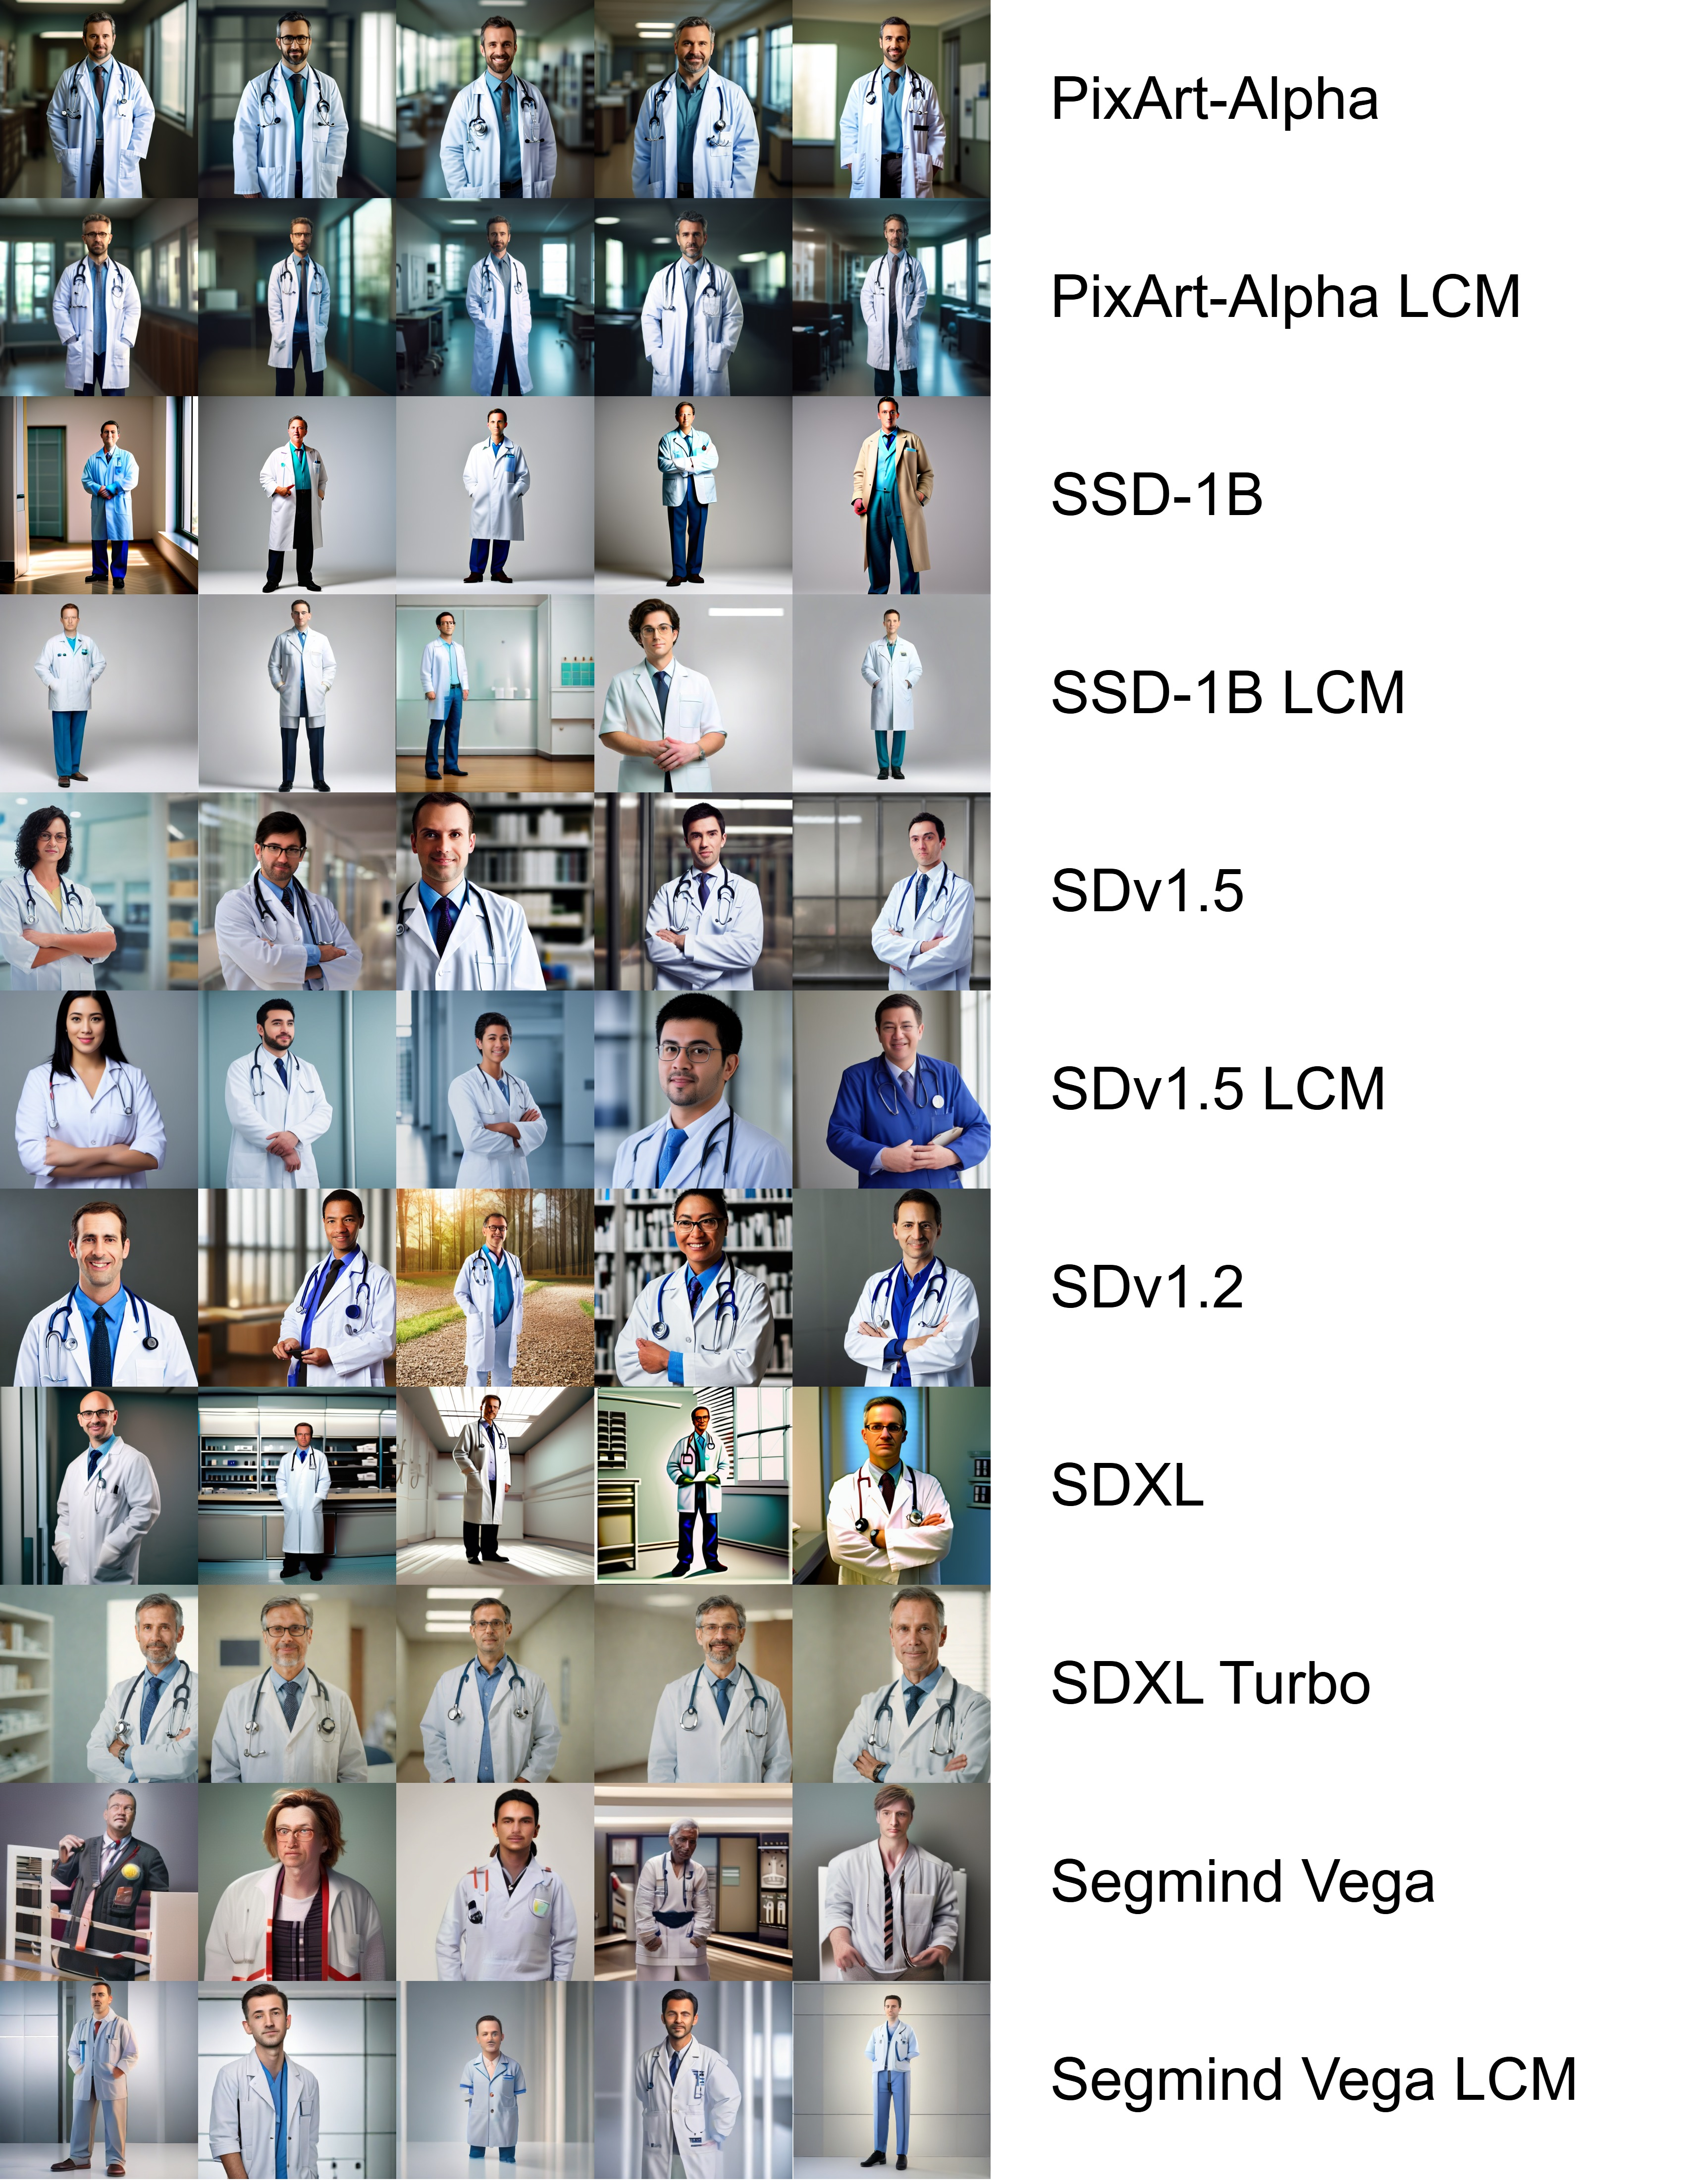
\includegraphics[width=\textwidth]{ImageGenerationSampleImages.jpg}
	\caption{Sample outputs from the ten model configurations screened
		during preliminary evaluation, generated using a fixed Doctor prompt
		at 512$\times$512 resolution. Four samples are shown per
		configuration. Of these, only SDv1.5, SDv1.5 LCM, and SDv1.2 satisfy
		the LAION training lineage criterion and are formally evaluated for
		model selection. The remaining configurations are included to
		illustrate the range of structural quality observed across the
		broader candidate set.}
	\label{fig:model_comparison_samples}
\end{figure}

SDv1.5 was therefore selected as the base model. It was loaded with the
\texttt{latent-consistency/lcm-lora-sdv1-5} adapter~\cite{LCMLoRA_SDv15}
and fused for fast inference, eliminating adapter overhead at generation
time. The default DDPM scheduler was replaced with \texttt{LCMScheduler},
which enables high-quality generation at substantially reduced step counts
through consistency distillation~\cite{Luo_2023_LCMLoRA}. A four-step
inference schedule was used for all validated generation runs; preliminary
testing confirmed that fewer than four steps introduces visible distortion,
while additional steps beyond four yield no measurable improvement in
structural quality. Generation was performed in half-precision (FP16) on
GPU, with TF32 enabled for matrix multiplications and cuDNN operations to
maximise throughput without sacrificing numerical precision.

%\subsection{Prompt Design and Justification}
%
%The prompt template used for all profession-conditioned generation was:
%
%\begin{quote}
%	\texttt{full-body realistic photo of a \{profession\}, standing, centered,
%		in a professional setting appropriate for their occupation, sharp focus,
%		35mm lens, natural professional lighting}
%\end{quote}
%
%Each component was chosen for a specific functional or fairness-related
%reason.
%
%\paragraph{Full-body framing.} Stable Diffusion models trained on
%LAION-scale data exhibit a strong prior toward portrait-style close-ups.
%Explicitly specifying full-body framing overrides this default and ensures
%compatibility with downstream structural validation, which requires a full
%detected person bounding box to confirm subject completeness.
%
%\paragraph{Standing, centered.} Explicit pose and spatial positioning
%tokens reduce compositional ambiguity arising from multiple subjects or
%edge-cropping artefacts. These constraints increase the probability that
%the detected face falls within the upper half of the person bounding box,
%satisfying the anatomical plausibility check applied during structural
%validation.
%
%\paragraph{Professional setting appropriate for their occupation.} Rather
%than specifying concrete environments (e.g., hospital, courtroom), which
%are known to amplify demographic stereotypes by conditioning the model on
%environment-associated appearance priors~\cite{Naik_2023_SocialBiasesThroughTheTextToImageGenerationLens},
%an abstract contextual phrase was used. This preserves profession-relevant
%semantic grounding while limiting activation of environment-specific
%demographic shortcuts.
%
%\paragraph{Sharp focus.} The four-step LCM sampling schedule can introduce
%diffusion-specific blur. High-frequency cues such as sharp focus improve
%edge fidelity, increasing the reliability of downstream face and person
%detection.
%
%\paragraph{35mm lens.} Camera focal-length tokens act as implicit geometric
%priors, influencing subject distance and body proportions. A 35mm
%specification promotes naturalistic perspective and full-body framing
%without barrel or perspective distortion.
%
%\paragraph{Natural professional lighting.} Lighting conditions significantly
%influence CLIP-based aesthetic scores and detection confidence. Neutral
%professional lighting tokens suppress noise artefacts and promote image
%quality scores that meet the downstream aesthetic filtering threshold.

\subsection{Prompt Design and Justification}

The prompt template used for all profession-conditioned generation was:

\begin{quote}
	\texttt{full-body realistic photo of a \{profession\}, standing, centered,
		in a professional setting appropriate for their occupation, sharp focus,
		35mm lens, natural professional lighting}
\end{quote}

Each component was chosen for a specific functional or fairness-related
reason.

\paragraph{Full-body framing.}
Stable Diffusion models trained on LAION-scale data exhibit a strong prior
toward portrait-style close-ups, a compositional tendency that arises from
the framing distribution of images in the training
corpus~\cite{Rombach_2022_CVPR}. Explicitly specifying full-body framing
overrides this default and ensures compatibility with downstream structural
validation, which requires a full detected person bounding box to confirm
subject completeness. Under-specified prompts have been shown to frequently
yield incomplete or cropped subjects; explicit body-level constraints
significantly improve compositional correctness in text-to-image
models~\cite{Chen_2023_T2ICompBench}.

\paragraph{Standing, centered.}
Explicit pose and spatial positioning tokens reduce compositional ambiguity
arising from multiple subjects or edge-cropping
artefacts~\cite{Nichol_2022_GLIDE, Chen_2023_T2ICompBench}. These
constraints increase the probability that the detected face falls within
the upper half of the person bounding box, satisfying the anatomical
plausibility check applied during structural validation. Without such
constraints, YOLO-based validation frequently fails when faces appear near
image borders, subjects are partially outside the frame, or multiple people
are unintentionally generated.

\paragraph{Professional setting appropriate for their occupation.}
Rather than specifying concrete environments (e.g., hospital, courtroom),
which are known to amplify demographic stereotypes by conditioning the model
on environment-associated appearance priors~\cite{Luccioni_2023_AnalyzingSocietalRepresentationsDiffusionModels} 
%\cite{Luccioni_2023_StableBias},
an abstract contextual phrase was used. Friedrich et
al.~\cite{Friedrich_2023_FairDiffusionInstructingTextToImage} recommend abstract role-appropriate
context as a means of reducing stereotype amplification while preserving
semantic coherence, and Luccioni et al.~\cite{Luccioni_2023_AnalyzingSocietalRepresentationsDiffusionModels} %\cite{Luccioni_2023_StableBias}
demonstrate empirically that explicit environment tokens correlate with
skewed demographic representations in diffusion outputs. This prompt
component therefore preserves profession-relevant semantic grounding while
limiting activation of environment-specific demographic shortcuts.

\paragraph{Sharp focus.}
The four-step LCM sampling schedule can introduce diffusion-specific blur,
a known degradation mode at low step counts~\cite{Luo_2023_LCMLoRA}.
High-frequency cues such as sharp focus improve edge fidelity, increasing
the reliability of downstream face and person detection. Blur directly
reduces CLIP aesthetic scores, YOLO face and person detection confidence,
and overall valid image yield.

\paragraph{35mm lens.}
Camera focal-length tokens act as implicit geometric priors, influencing
subject distance and body proportions~\cite{Fang_2024_CameraTokens}.
A 35mm specification promotes naturalistic perspective and full-body
framing without barrel or perspective distortion, increasing the probability
of full-body framing and compatibility with face--person spatial
validators~\cite{Chen_2023_T2ICompBench}.

\paragraph{Natural professional lighting.}
Lighting conditions significantly influence CLIP-based aesthetic scores and
detection confidence~\cite{Schuhmann_2022_LaionAesthetics}. Neutral
professional lighting tokens suppress noise artefacts, improve edge
definition under low-step sampling, and promote image quality scores that
meet the downstream aesthetic filtering threshold~\cite{Friedrich_2023_FairDiffusionInstructingTextToImage}.

\subsection{Guidance Scale and Its Methodological Implications}

The classifier-free guidance scale was fixed at $s = 1.0$ across all
validated generation runs. At $s = 1$, no guidance amplification is
applied, and the model produces outputs conditioned purely on its learned
prior without any prompt-signal exaggeration.

Standard Stable Diffusion deployment uses guidance scales in the range
$s = 7$--$7.5$. This choice was deliberate. As described in
Section~\ref{subsec:cfg}, classifier-free guidance is an inference-time
amplification mechanism that scales the difference between conditional and
unconditional predictions; elevated guidance increases prompt adherence but
also amplifies any demographic or compositional bias encoded in the learned
prior. By fixing $s = 1$, the generated distribution reflects the model's
intrinsic learned associations rather than inference-time amplifications of
those associations. As a consequence, any demographic bias identified under
$s = 1$ represents a conservative lower bound: at guidance scales used in
production deployment, the same biases would be further amplified. If bias
is detectable at its minimum---when guidance amplification is absent---it
follows that the bias is structural and attributable to model weights and
training data, not to inference-time configuration.

This stands in contrast to the unconditional control subset, which was
generated with $s = 0.0$ and an empty prompt, producing samples from the
model's learned prior without any profession conditioning. The guidance
scale argument is therefore specific to the profession-conditioned runs;
the control subset serves a different purpose and is not subject to the
same inference-time amplification concern.

\subsection{Asynchronous Generation and Validation Architecture}
\label{subsec:async_architecture}

Images were generated for each of the 200 professions in batches of 2. For
each profession, generation continued until 1{,}000 structurally valid
images had been accepted. To avoid blocking GPU generation during
CPU-bound validation, structural validation was decoupled from generation
using an asynchronous producer--consumer architecture.

A \texttt{ValidationWorker} pool was instantiated with a configurable
number of worker threads (default: 2). Each worker thread independently
loaded its own copies of the YOLO person detection model, YOLO face
detection model, and MediaPipe FaceMesh. Validation tasks were submitted to
a shared task queue and results returned via a result queue, allowing the
main GPU generation loop to remain active while CPU workers processed
previously generated images in parallel. Generated images were held in an
in-memory cache keyed by unique image identifier, and retrieved for saving
or discarding once the corresponding validation result arrived. File I/O
was performed asynchronously via a separate thread pool executor with 4
workers to avoid blocking either generation or validation.

Per-profession resumability was implemented as a property of this
architecture. At the start of each profession, the pipeline counted
existing valid images in the output directory; if the target count of
1{,}000 had already been reached, the profession was skipped without
re-running generation. This design tolerated interruptions across the full
200-profession generation run without requiring any previously accepted
images to be regenerated.

\subsection{Structural Validation Criteria and Unfiltered Control Subset}
\label{subsec:structural_validation}

Unlike retrieval from Re-LAION-5B, generative models produce images without
guarantees of compositional suitability. Common failure modes include
multiple subjects, truncated bodies, disconnected or misaligned faces,
anatomically inconsistent compositions, and low-frequency blurred
renderings arising from low-step inference. Since downstream demographic
and spurious feature analysis requires clearly identifiable single
individuals in consistent compositional configurations, structural
validation is a necessary preprocessing stage for profession-conditioned
generated images. The parallel validation architecture described in
Section~\ref{subsec:async_architecture} ensures that this filtering does
not constitute a throughput bottleneck.

An image was accepted only if it satisfied all of the following conditions.

\paragraph{Person detection.} The YOLO person detection model
(\texttt{yolo12s.pt}) must detect at least one bounding box with class ID
0 and confidence $\geq 0.4$.

\paragraph{Face detection.} The YOLO face detection model
(\texttt{yolov12l-face.pt}) must detect exactly one face with confidence
$\geq 0.4$. Images with zero or multiple detected faces were rejected.

\paragraph{Face crop validity.} The face bounding box must define a
non-empty region of interest. Degenerate crops of zero area were rejected.

\paragraph{FaceMesh segmentation.} MediaPipe FaceMesh (configured with
\texttt{static\_image\_mode=True}, \texttt{max\_num\_faces=1}, and
\texttt{refine\_landmarks=True}) must successfully return landmarks for the
face region of interest, with a minimum of 10 landmark points. Landmarks
were used to compute a convex hull mask over the face, from which a tightly
cropped segmented face ROI was extracted with a 10-pixel boundary padding.

\paragraph{Spatial and anatomical consistency.} For each detected person
bounding box, a composite spatial score was computed:

\[
\text{score} = 10 \cdot \mathbf{1}[\text{centroid\_inside}] + 2 \cdot
\mathbf{1}[\text{upper\_half}] + \min\!\left(\frac{A_\text{face}}{A_\text{person}},\,
0.05\right) \cdot 20
\]

where $\mathbf{1}[\text{centroid\_inside}]$ indicates that the face
centroid lies within the person bounding box, $\mathbf{1}[\text{upper\_half}]$
indicates that the face centroid lies in the upper half of the person
bounding box (an anatomical plausibility constraint), and
$A_\text{face}/A_\text{person}$ is the face-to-person area ratio. The
person bounding box with the highest score was selected as the candidate
association. If the face centroid did not fall within the candidate bounding
box, an expanded bounding box (expanded 5\% horizontally, 15\% vertically
from the top edge) was tested. Images for which no valid person--face
spatial association could be established were rejected. Additionally, the
face-to-person area ratio must exceed $0.002$ to prevent association with
degenerate detections.

\paragraph{Aesthetic quality.} Following successful structural validation,
each accepted image was scored using a CLIP-based aesthetic regressor.
Image features were extracted using \texttt{open\_clip} with the ViT-L-14
backbone pretrained on LAION-2B (\texttt{laion2b\_s32b\_b82k}), and
projected to a scalar aesthetic score via a lightweight linear head
(\texttt{sa\_0\_4\_vit\_l\_14\_linear.pth}) trained to predict human
aesthetic preference ratings. Images with an aesthetic score below 3.0 were
rejected, as described in Section~\ref{subsec:aesthetic_scoring}.

Images passing all criteria were saved to disk along with their
corresponding FaceMesh face crops. Rejected images were stored in a
separate invalid directory with the rejection reason encoded in the
filename, enabling post-hoc analysis of failure mode distributions. A CSV
metadata file was written incrementally, recording image filename,
profession label, aesthetic score, face bounding box, and person bounding
box for each accepted image.

To provide an unfiltered counterpart to the validated profession-conditioned
set, a separate control set of 10{,}000 images was generated using blank
prompts with none of the above validation constraints applied. The inference
configuration was otherwise identical: Stable Diffusion v1.5 with LCM
LoRA, four inference steps, and FP16 precision. The guidance scale was set
to $s = 0.0$, yielding unconditional samples drawn from the model's learned
prior with no prompt conditioning applied. These images carry no
profession-specific semantic signal and are subject to none of the
compositional constraints imposed by the generation prompt; they may depict
people, objects, scenes, or abstract content, mirroring the unconstrained
character of the Re-LAION-5B random control subset described in
Section~\ref{subsec:subset_design}. Images were saved directly to disk as
produced, preserving the raw generative distribution without any
human-centric filtering. The purpose and analytical role of this control
subset are identical to those of the Re-LAION-5B control: to assess whether
spurious low-level features identified in the validated
profession-conditioned images generalise to images generated without any
human-centric constraint, and to enable direct comparison of the degree to
which spurious correlations present in the training data are reproduced in
model outputs.

\subsection{Structural Acceptance Rates for Generated Images}

Following generation and validation, acceptance rates were computed per
profession using the same methodology as the Re-LAION-5B retrieval
analysis. Across all 200 professions, the mean structural acceptance rate
for generated images was 66.38\%, with a median of 71.00\% and a standard
deviation of 16.60\%. Acceptance rates ranged from approximately 10\% to
over 90\%.

Figure~\ref{fig:sd_acceptance_histogram} illustrates the distribution of
acceptance rates across professions. Compared to retrieval from Re-LAION-5B
(mean acceptance 33.51\%), generated images exhibit substantially higher
structural validity. This is consistent with the effect of the full-body
prompt engineering, which biases the diffusion model toward compositions
that satisfy single-person detection and face--person spatial association
requirements. Nonetheless, per-profession variability remains substantial,
indicating that certain occupations activate compositional priors within
the model that systematically resist full-body single-subject framing. The
systematic difference in mean acceptance rate between retrieved (33.51\%)
and generated (66.38\%) subsets must be considered when comparing
demographic or spurious feature prevalence across the two data sources, as
the structural filtering stage does not operate identically across the two
pipelines.

\begin{figure}[htbp]
	\centering
	\includegraphics[width=\textwidth]{SD-Distribution.png}
	\caption{Distribution of structural acceptance rates across 200 professions
		for Stable Diffusion v1.5 generated images following YOLO-based structural
		validation and aesthetic filtering. The distribution is left-skewed with a
		mean of 66.38\% and median of 71.00\%, substantially higher than the
		Re-LAION-5B retrieval acceptance rate of 33.51\%, consistent with the
		effect of full-body prompt engineering on generative composition.}
	\label{fig:sd_acceptance_histogram}
\end{figure}

% ============================================================
%  Section: Demographic Annotation
%  Subsections: Pre-processing, Gender Annotation, Skin Tone Annotation
% ============================================================
%
% Citation TODOs (not present in references.bib — add entries before submission):
%   TODO_CCv2          : Hazirbas et al. 2022, "Casual Conversations v2", Meta AI
%   TODO_FACET         : Gustafson et al. 2023, "Facet: Fairness in Computer Vision Evaluation Benchmark"
%   TODO_VGG16         : Simonyan & Zisserman 2015, "Very Deep Convolutional Networks for Large-Scale Image Recognition"
%   TODO_DenseNet      : Huang et al. 2017, "Densely Connected Convolutional Networks"
%   TODO_DeepFace      : Serengil & Ozpinar 2020, DeepFace
%   TODO_InsightFace   : Deng et al. 2020, InsightFace
%   TODO_HFGender      : rizvandwiki/gender-classification (HuggingFace model card)
%   TODO_RealisticGndr : prithivMLmods/Realistic-Gender-Classification (HuggingFace model card)
%   TODO_SkinToneLib   : skin-tone-classifier PyPI library
% ============================================================

\newpage\section{Demographic Annotation}
\label{sec:demographic_annotation}

To enable bias analysis across gender and skin tone dimensions, every face-containing image in both the Re-LAION-5B retrieval set and the Stable Diffusion v1.5 generation set required demographic labels. This section describes the common pre-processing applied to all annotation tasks, the candidate model evaluation procedure used to select a gender classifier, and the equivalent evaluation used to select a skin tone estimator, including the ablation study conducted on the best-performing architecture.

% -----------------------------------------------------------
\subsection{Pre-processing}
\label{sec:annotation_preprocessing}

All images, prior to either gender or skin tone inference, were passed through a consistent face segmentation step using MediaPipe FaceMesh~\cite{Kartynnik_2019_FaceMesh}. FaceMesh fits a dense 468-landmark mesh to the detected face region and returns a per-pixel membership mask, from which a convex hull was computed. Pixels outside the hull were replaced with a uniform black fill, yielding a tightly cropped, background-removed face image that served as the input to all annotation models. This is the same FaceMesh configuration employed during structural validation (Section~\ref{subsec:structural_validation}), and the same face crop produced there was reused here, ensuring that both annotation tasks operated on identical inputs.

Applying segmented face crops rather than full bounding-box crops serves two purposes. First, models evaluated on unsegmented crops are susceptible to learning background cues that correlate incidentally with demographic attributes rather than the facial features the annotation is intended to capture~\cite{Matias_2024_EnhancingFairnessMST}; masking the background removes this failure case. Second, a uniform pre-processing step ensures that any observed accuracy differences across candidate models reflect genuine differences in representational capacity rather than differences in the image region each model receives.

For the FACET benchmark~\cite{Gustafson_2023_FACET}, an additional filtering step was applied prior to model evaluation: only samples with an annotator-consensus score of at least 2.0 were retained. FACET provides per-sample consensus scores that reflect inter-annotator agreement on the ground-truth labels; retaining only high-agreement samples suppresses label noise that would otherwise inflate per-model error rates independently of the models being compared.

% -----------------------------------------------------------
\subsection{Gender Annotation}
\label{sec:gender_annotation}

\subsubsection{Candidate Models}

Five off-the-shelf gender classifiers were evaluated on segmented face crops:

\begin{enumerate}
	\item \textbf{HuggingFace Gender Classifier}~\cite{Rizvandwiki_2023_HuggingFaceGenderClassification} --- a ViT-B/16 model fine-tuned for binary gender classification.
	\item \textbf{Realistic Gender Classifier}~\cite{Tschannen_2025_SigLIP2_RealisticGenderClassifier} --- a SigLIP-backbone classifier trained on high-quality portrait imagery.
	\item \textbf{DeepFace}~\cite{Serengil_2021_HyperExtendedLightFace_DeepFace} --- a multi-attribute facial analysis library providing gender prediction as one of several demographic attributes.
	\item \textbf{InsightFace}~\cite{Deng_2022_ArcFace_InsightFace} --- a face analysis toolkit with an integrated demographic attribute head.
	\item \textbf{FairFace}~\cite{Karkkainen_2021_FairFace} --- a classifier trained on a demographically balanced dataset, explicitly designed to reduce cross-group accuracy disparities.
\end{enumerate}

\subsubsection{Evaluation Protocol}

Models were evaluated on the Casual Conversations v2 (CCv2)~\cite{Porgali_2023_CCv2} and FACET~\cite{Gustafson_2023_FACET} datasets, both pre-processed as described above. DeepFace does not expose a batched inference interface and was therefore evaluated exclusively on FACET, where the smaller sample count made serial single-image inference tractable. For CCv2, two evaluation conditions were defined: \emph{full images} (the original dataset images without segmentation) and \emph{face-only crops} (the FaceMesh-segmented face regions). The face-only condition matches the inputs the annotation pipeline operates on; the full-image condition is reported for reference. Accuracy was computed as the proportion of correct binary predictions, and was decomposed into male and female subgroup rates to surface asymmetric error behaviour.

\subsubsection{Results}

Table~\ref{tab:gender_results} summarises overall and per-class accuracy across models. Results are reported for the CCv2 face-only (segmented) condition and FACET, both of which correspond to the segmented input format used during final annotation.

\begin{table}[htbp]
	\centering
	\caption{Gender classification accuracy on CCv2 face-only segmented crops and FACET. Overall, male (M), and female (F) accuracies are reported. DeepFace was not evaluated on CCv2 face-only due to the absence of a batch inference interface. The Realistic Gender Classifier achieves the highest overall accuracy on CCv2 face-only and the best balance between male and female subgroup accuracy.}
	\label{tab:gender_results}
	\begin{tabular}{lccccccc}
		\toprule
		& \multicolumn{3}{c}{\textbf{CCv2 Face-Only}} & & \multicolumn{3}{c}{\textbf{FACET}} \\
		\cmidrule(lr){2-4} \cmidrule(lr){6-8}
		\textbf{Model} & \textbf{Overall} & \textbf{M} & \textbf{F} & & \textbf{Overall} & \textbf{M} & \textbf{F} \\
		\midrule
		HF Gender Classifier   & 0.715 & 0.963 & 0.561 & & 0.789 & 0.877 & 0.569 \\
		Realistic Gender Clf.  & \textbf{0.886} & \textbf{0.924} & \textbf{0.862} & & 0.823 & 0.875 & 0.695 \\
		InsightFace            & 0.771 & 0.784 & 0.763 & & 0.772 & 0.821 & 0.643 \\
		FairFace               & 0.801 & 0.983 & 0.687 & & \textbf{0.834} & \textbf{0.906} & 0.653 \\
		DeepFace               & ---   & ---   & ---   & & 0.780 & 0.938 & 0.384 \\
		\bottomrule
	\end{tabular}
\end{table}

The Realistic Gender Classifier achieved an overall accuracy of 88.6\% on the CCv2 face-only set, with a male accuracy of 92.4\% and a female accuracy of 86.2\%, a male--female gap of 6.2 percentage points. This gap is substantially smaller than those of the HuggingFace classifier (40.2 pp), FairFace (29.6 pp), and DeepFace on FACET (55.4 pp), all of which exhibit a systematic tendency to classify ambiguous or darker-toned faces as male. InsightFace achieved the smallest male--female gap (2.1 pp on CCv2 face-only) but at the cost of a 11.5 percentage point reduction in overall accuracy relative to the Realistic Gender Classifier, indicating that its more balanced per-class rates arise from lower male recall rather than improved female recall.

\subsubsection{Per-Skin-Tone Performance of the Selected Model}

Table~\ref{tab:gender_skintone} disaggregates the Realistic Gender Classifier's CCv2 face-only accuracy by MST level. This disaggregation is relevant to the downstream analysis, as it quantifies the degree to which annotation quality varies across the same demographic dimension the thesis analyses.

\begin{table}[htbp]
	\centering
	\caption{Per-MST-level accuracy of the Realistic Gender Classifier on CCv2 face-only segmented crops. Overall, male (M), and female (F) sub-group accuracies and sample counts (N) are reported. Accuracy is highest for mid-range tones (MST~4--6) and degrades at both extremes, with female accuracy declining more sharply at darker tones.}
	\label{tab:gender_skintone}
	\small
	\begin{tabular}{lcccc}
		\toprule
		\textbf{MST} & \textbf{N} & \textbf{Overall} & \textbf{M Acc.} & \textbf{F Acc.} \\
		\midrule
		1  & 1{,}190  & 0.756 & 0.977 & 0.681 \\
		2  & 13{,}337 & 0.870 & 0.968 & 0.833 \\
		3  & 33{,}732 & 0.893 & 0.946 & 0.870 \\
		4  & 38{,}273 & 0.893 & 0.939 & 0.871 \\
		5  & 55{,}797 & 0.906 & 0.918 & 0.895 \\
		6  & 23{,}074 & 0.879 & 0.884 & 0.875 \\
		7  & 6{,}438  & 0.826 & 0.906 & 0.761 \\
		8  & 4{,}183  & 0.803 & 0.925 & 0.680 \\
		9  & 1{,}671  & 0.662 & 0.948 & 0.488 \\
		10 & 168      & 0.726 & 1.000 & 0.570 \\
		\bottomrule
	\end{tabular}
\end{table}

Overall accuracy peaks at MST~5 (90.6\%) and declines toward both the lightest and darkest tones, falling to 75.6\% at MST~1 and 66.2\% at MST~9. Male accuracy remains consistently high across all MST levels, ranging from 88.4\% at MST~6 to 100.0\% at MST~10, with no systematic degradation at darker tones, while female accuracy degrades sharply from 87.5\% at MST~6 to 48.8\% at MST~9, consistent with the intersectional accuracy disparities documented in prior work on face-based classification~\cite{Buolamwini_2018_BiasGenderClassification, Buolamwini_2018_GenderShades}. These limitations must be accounted for when interpreting gender-disaggregated results at the darker end of the skin tone range, particularly for female subgroups.

Despite these disparities, the Realistic Gender Classifier offered the best combination of overall accuracy, male--female balance, and inference throughput among the five evaluated candidates, and was therefore selected for final annotation.

% -----------------------------------------------------------
\subsection{Skin Tone Annotation}
\label{sec:skintone_annotation}

\subsubsection{Scale Selection}

Prior to model evaluation, a choice between the two most widely used skin tone measurement scales in the fairness literature was required. The Fitzpatrick scale~\cite{Fitzpatrick_1988_SkinTypes} partitions skin into six phototype categories originally developed to predict ultraviolet radiation sensitivity, and while it has seen broad adoption in computer vision, it has been criticised for conflating clinical and perceptual dimensions and for providing insufficient resolution to distinguish dark skin tones reliably~\cite{Schumann_2024_MonkSkinTone}. The Monk Skin Tone (MST) scale~\cite{Schumann_2024_MonkSkinTone} provides a ten-point ordinal scale developed with representational equity as an explicit design objective.

Heldreth et al.~\cite{Heldreth_2024_WhichSkinToneMeasures} conducted a large-scale survey comparing the Fitzpatrick, MST, and Fenty Beauty (40-point) scales across 2{,}214 US participants, finding that the Fitzpatrick scale was perceived as significantly less inclusive by darker-skinned, non-White, and female respondents, while the MST and Fenty scales were rated comparably despite the large difference in granularity. On the basis of these findings, the MST scale was adopted for this work.

Skin tone predictions were produced as raw ten-point MST scores (MST~1--10) and additionally collapsed into a three-bin grouping following the convention of Matias and Neto~\cite{Matias_2024_EnhancingFairnessMST}: Light (MST~1--3), Mid (MST~4--7), and Dark (MST~8--10). The three-bin representation is used for all aggregate bias analyses, as the coarser granularity is more robust to annotation noise and aligns with the groupings used in the related fairness literature.

\subsubsection{Candidate Models}

Four skin tone estimation approaches were evaluated:

\begin{enumerate}
	\item \textbf{SkinTone Classifier Library} --- an off-the-shelf Python library that derives MST estimates from colour histograms over the face region; applied directly without training ~\cite{Pina_2023_SkinToneClassificationLibrary}.
	\item \textbf{RandomForest} --- a histogram-based regressor trained on 256-bin per-channel colour features extracted from segmented face crops, following the methodology of Matias and Neto~\cite{Matias_2024_EnhancingFairnessMST}. Trained on CCv2.
	\item \textbf{DenseNet-121} --- a densely connected convolutional network trained for MST classification in LAB colour space, following the architecture evaluated by Matias and Neto~\cite{Matias_2024_EnhancingFairnessMST}. Trained on CCv2.
	\item \textbf{VGG-16} --- a deep convolutional network fine-tuned for MST estimation, adapted from the architecture evaluated by Mbatha et al.~\cite{Mbatha_2024_SkinToneLighting} in the context of skin tone estimation under diverse lighting conditions. Trained on CCv2 and subsequently ablated across four design axes.
\end{enumerate}

All trained models were evaluated on a held-out CCv2 validation split, the Monk Skin Tone Estimation (MSTE) benchmark~\cite{Mbatha_2024_SkinToneLighting}, and FACET~\cite{Gustafson_2023_FACET}. Three metrics were computed for each model--dataset combination: exact accuracy, within-one accuracy (prediction within one MST step of the ground truth), and three-bin accuracy (prediction in the correct Light/Mid/Dark bin).

\subsubsection{Baseline Results}

Table~\ref{tab:skintone_baseline} reports global accuracy for the SkinTone Classifier Library, RandomForest, and DenseNet-121 across the three evaluation datasets.

\begin{table}[htbp]
	\centering
	\caption{Global accuracy of baseline skin tone models. E = exact, ±1 = within-one, B = three-bin. All trainable models were trained on CCv2. The SkinTone Library requires no training.}
	\label{tab:skintone_baseline}
	\begin{tabular}{lccccccccc}
		\toprule
		& \multicolumn{3}{c}{\textbf{MSTE}} & \multicolumn{3}{c}{\textbf{CCv2}} & \multicolumn{3}{c}{\textbf{FACET}} \\
		\cmidrule(lr){2-4} \cmidrule(lr){5-7} \cmidrule(lr){8-10}
		\textbf{Model} & E & ±1 & B & E & ±1 & B & E & ±1 & B \\
		\midrule
		SkinTone Library & 0.112 & 0.281 & 0.425 & 0.084 & 0.298 & 0.603 & 0.073 & 0.239 & 0.421 \\
		RandomForest     & 0.132 & 0.335 & 0.410 & 0.346 & 0.756 & 0.700 & 0.176 & 0.550 & 0.484 \\
		DenseNet-121     & 0.210 & 0.517 & 0.564 & 0.303 & 0.692 & 0.697 & 0.210 & 0.529 & 0.576 \\
		\bottomrule
	\end{tabular}
\end{table}

The SkinTone Classifier Library performs poorly across all datasets and metrics. The low MSTE exact accuracy (11.2\%) despite higher CCv2 three-bin accuracy (60.3\%) reflects a tendency to predict a narrow range of mid-scale values that coincidentally aligns with the mid-tone skew of the CCv2 training distribution but not the more balanced MSTE distribution. Per-tone analysis confirms that the library assigns near-zero prediction probability to MST~1--3 across all datasets, rendering it unsuitable for tasks requiring reliable coverage of light skin tones.

The RandomForest achieves substantially higher within-one accuracy on CCv2 (75.6\%) than on MSTE (33.5\%) or FACET (55.0\%), indicating overfitting to the CCv2 training distribution. Per-tone results show that predictions are concentrated in MST~4--6, with near-zero accuracy for MST~1--3 and MST~8--10, which constitute a small proportion of the CCv2 training distribution. DenseNet-121 generalises more evenly across the tone range, with comparable MSTE and FACET three-bin accuracies (56.4\% and 57.6\%), but remains the second-weakest overall. The best-performing VGG-16 configuration exceeded DenseNet-121 on all CCv2 metrics, as shown in Table~\ref{tab:vgg16_mst10}, and VGG-16 was therefore selected for further optimisation via the ablation study described below.

\subsubsection{VGG-16 Ablation Study}
\label{sec:vgg16_ablation}

A factorial ablation was conducted across four binary design dimensions, yielding sixteen VGG-16 variants evaluated under two label spaces (MST10 and MST3). The four axes were:

\begin{itemize}
	\item \textbf{Output formulation}: \emph{classification} (softmax cross-entropy over $K$ discrete classes) versus \emph{regression} (mean squared error over a continuous scalar clamped to $[1, 10]$ for MST10, with predictions rounded to the nearest integer at inference time).
	\item \textbf{Colour space}: \emph{RGB} versus \emph{CIE L*a*b*} (LAB). LAB decouples luminance from chrominance, which Mbatha et al.~\cite{Mbatha_2024_SkinToneLighting} found to improve robustness to lighting variation in skin tone estimation.
	\item \textbf{Label granularity}: MST10 (ten classes) versus MST3 (three-bin Light/Mid/Dark labels).
	\item \textbf{Background}: \emph{black background} (uniform black fill outside the face hull) versus \emph{average skin-tone background} (background pixels set to the mean colour of unmasked face pixels), motivated by the hypothesis that high-contrast face--background boundaries in the black condition may bias convolutional filters toward edge rather than colour features.
\end{itemize}

Tables~\ref{tab:vgg16_mst10} and~\ref{tab:vgg16_mst3} report results for representative variants across both label spaces.

\begin{table}[htbp]
	\centering
	\caption{VGG-16 MST10 variant accuracy across all eight design axis combinations. E = exact, ±1 = within-one, B = three-bin. BB = black background, AB = average skin-tone background. All models trained on CCv2. Bold indicates the best value in each column.}
	\label{tab:vgg16_mst10}
	\small
	\begin{tabular}{llccccccccc}
		\toprule
		& & \multicolumn{3}{c}{\textbf{MSTE}} & \multicolumn{3}{c}{\textbf{CCv2}} & \multicolumn{3}{c}{\textbf{FACET}} \\
		\cmidrule(lr){3-5} \cmidrule(lr){6-8} \cmidrule(lr){9-11}
		\textbf{Mode} & \textbf{Space / BG} & E & ±1 & B & E & ±1 & B & E & ±1 & B \\
		\midrule
		Class. & RGB / BB & 0.161 & 0.423 & \textbf{0.577} & 0.336 & 0.717 & 0.735 & 0.172 & 0.465 & 0.587 \\
		Class. & RGB / AB & 0.217 & 0.445 & 0.529 & 0.341 & 0.636 & 0.717 & 0.119 & 0.384 & 0.547 \\
		Class. & LAB / BB & \textbf{0.228} & 0.493 & 0.568 & 0.346 & 0.697 & 0.723 & 0.145 & 0.437 & 0.544 \\
		Class. & LAB / AB & 0.162 & 0.445 & 0.492 & 0.283 & 0.669 & 0.674 & 0.148 & 0.442 & 0.583 \\
		Regr.  & RGB / BB & 0.159 & 0.424 & 0.566 & \textbf{0.375} & \textbf{0.804} & 0.778 & 0.165 & 0.471 & 0.593 \\
		Regr.  & RGB / AB & 0.132 & 0.367 & 0.528 & 0.374 & 0.784 & \textbf{0.783} & 0.173 & 0.499 & 0.572 \\
		Regr.  & LAB / BB & 0.146 & 0.423 & 0.549 & 0.350 & 0.776 & 0.734 & 0.185 & 0.532 & 0.587 \\
		Regr.  & LAB / AB & 0.163 & \textbf{0.494} & 0.556 & 0.370 & 0.778 & 0.775 & \textbf{0.207} & \textbf{0.567} & \textbf{0.596} \\
		\bottomrule
	\end{tabular}
\end{table}

\begin{table}[htbp]
	\centering
	\caption{VGG-16 MST3 variant accuracy across all eight design axis combinations. Since the label space contains only three classes, exact accuracy and three-bin accuracy are identical; ±1 reflects predictions within one bin of the true bin. BB = black background, AB = average skin-tone background. All models trained on CCv2. Bold indicates the best value in each column.}
	\label{tab:vgg16_mst3}
	\small
	\begin{tabular}{llcccccc}
		\toprule
		& & \multicolumn{2}{c}{\textbf{MSTE}} & \multicolumn{2}{c}{\textbf{CCv2}} & \multicolumn{2}{c}{\textbf{FACET}} \\
		\cmidrule(lr){3-4} \cmidrule(lr){5-6} \cmidrule(lr){7-8}
		\textbf{Mode} & \textbf{Space / BG} & Exact & ±1 & Exact & ±1 & Exact & ±1 \\
		\midrule
		Class. & RGB / BB & 0.557 & 0.939 & 0.771 & 0.994 & 0.583 & 0.983 \\
		Class. & RGB / AB & 0.545 & 0.945 & 0.765 & 0.993 & 0.581 & 0.972 \\
		Class. & LAB / BB & 0.478 & 0.883 & 0.723 & 0.957 & 0.534 & 0.944 \\
		Class. & LAB / AB & 0.540 & 0.901 & 0.727 & 0.990 & 0.502 & 0.908 \\
		Regr.  & RGB / BB & \textbf{0.627} & 0.992 & \textbf{0.801} & \textbf{1.000} & \textbf{0.640} & 0.996 \\
		Regr.  & RGB / AB & 0.584 & 0.978 & 0.799 & \textbf{1.000} & 0.619 & 0.997 \\
		Regr.  & LAB / BB & 0.578 & \textbf{0.996} & 0.749 & \textbf{1.000} & 0.604 & 0.997 \\
		Regr.  & LAB / AB & 0.526 & 0.995 & 0.777 & 0.999 & 0.598 & \textbf{0.998} \\
		\bottomrule
	\end{tabular}
\end{table}

\subsubsection{Model Selection}

The ablation results support three conclusions. First, the regression formulation outperforms classification on the metrics most relevant to downstream analysis. In the MST10 setting, the RGB regression model achieves a CCv2 within-one accuracy of 80.4\% and a three-bin accuracy of 77.8\%, compared to 71.7\% and 73.5\% for the classification variant. This advantage arises because regression produces a continuous output that is rounded to the nearest integer at inference time, distributing prediction probability smoothly across adjacent MST classes rather than committing fully to a single discrete class. Near class boundaries, where the true score falls between two adjacent MST values, this smooth degradation reduces the penalty incurred on within-one and three-bin metrics. Since the downstream analysis relies on three-bin groupings, regression's more graceful handling of boundary cases is methodologically preferable.

Second, RGB outperforms LAB as the input colour space. The LAB variants do not yield the improvements in MSTE accuracy that might be expected from luminance decoupling, suggesting that the CCv2 training distribution already provides sufficient implicit lighting variation to support luminance-robust representations. In the MST10 setting, the black background consistently matches or outperforms the average skin-tone background across regression variants. The clearest example is the MSTE three-bin comparison, where the average-background regression variant scores 52.8\% against 56.6\% for black background, a difference of 3.8 percentage points. This suggests that the additional colour introduced by filling the background with the mean face colour provides no representational benefit and may introduce low-frequency chrominance variation that partially confounds the skin tone signal. The advantage of black background is less consistent in the MST3 setting, where the coarser label space reduces sensitivity to within-variant differences.

Third, when comparing the final MST10 RGB regression model against the best MST3 model on three-bin accuracy --- the primary downstream metric --- the MST10 model achieves 77.8\% on CCv2 compared to 80.1\% for MST3 regression, a difference of 2.3 percentage points. This marginal improvement from MST3 comes at the cost of discarding all within-bin ordinal resolution; the MST10 model retains the continuous ten-point score as a secondary output, enabling finer-grained analysis if required.

The final selected model is therefore the \textbf{VGG-16 MST10 Regression RGB Black-Background} variant, achieving the following performance:

\begin{table}[htbp]
	\centering
	\caption{Final selected model performance summary: VGG-16 MST10 Regression RGB Black-Background.}
	\label{tab:vgg16_final}
	\begin{tabular}{lccc}
		\toprule
		\textbf{Dataset} & \textbf{Exact Acc.} & \textbf{Within-One Acc.} & \textbf{Three-Bin Acc.} \\
		\midrule
		CCv2 (held-out) & 0.375 & 0.804 & 0.778 \\
		MSTE            & 0.159 & 0.424 & 0.566 \\
		FACET           & 0.165 & 0.471 & 0.593 \\
		\bottomrule
	\end{tabular}
\end{table}

The lower MSTE and FACET exact accuracies relative to CCv2 reflect two compounding factors. The first is distributional shift: CCv2 exhibits an uneven MST distribution arising from its participant demographics and recording geography, meaning the model encountered certain tone ranges more frequently during training and generalises unevenly across the full ten-point scale. The second factor is more specific to MSTE. That dataset was designed so that the same subject receives an identical ground truth MST label regardless of lighting condition, precisely in order to test annotation consistency across illuminants. The model, however, was trained without explicit lighting augmentation and has no mechanism for illumination invariance. When MSTE presents the same face under spectrally distinct light sources, the model receives genuinely different pixel statistics and produces different predictions while the ground truth label remains fixed. The resulting accuracy drop is therefore not purely a sampling artefact but a direct consequence of photometric sensitivity encountering a benchmark engineered to expose it. Three-bin accuracy is more robust to both effects, as the broader grouping boundaries absorb within-class prediction variance and reduce sensitivity to the precise MST score assigned to individual samples.

\subsubsection{Final Annotation Pipeline}

The selected gender classifier and skin tone model were integrated into a unified annotation script. For each input image the pipeline executes the following operations in sequence: (1) the FaceMesh segmentation step described in Section~\ref{sec:annotation_preprocessing} produces a black-background face crop; (2) the Realistic Gender Classifier is applied to the RGB crop, yielding a binary gender label and a confidence score; (3) the VGG-16 MST10 Regression model is applied to the same RGB crop, yielding a continuous MST score that is rounded to the nearest integer for discrete-class reporting and subsequently mapped to the Light/Mid/Dark bin; and (4) the resulting labels --- gender, continuous MST score, integer MST class, and three-bin skin tone category --- are written to a per-image JSONL manifest. The pipeline supports GPU batch inference and is fully resumable via the manifest file.

This pipeline was applied to the complete sets of face-containing images retrieved from Re-LAION-5B and generated by Stable Diffusion v1.5, producing the demographic labels used in all subsequent bias analyses.

% ============================================================
% Section 3.4.4 — Real-World Occupational Demographic Reference Data
% ============================================================

\subsection{Real-World Occupational Demographic Reference Data}
\label{subsec:bls_reference}

To contextualise observed demographic distributions against ground-truth labour force
composition, two complementary reference datasets were derived: a US-specific baseline
sourced from the Bureau of Labor Statistics, and a global baseline sourced from the
International Labour Organization. The US baseline serves as the primary reference due
to the Western-web-dominated composition of Re-LAION-5B and its direct comparability
with prior work on occupational bias in text-to-image models~\cite{Bianchi_2023_EasilyAccessibleTextToImageModels,
	Luccioni_2023_AnalyzingSocietalRepresentationsDiffusionModels}. The global baseline
provides a cross-cultural robustness check; where the two baselines converge on the
same directional conclusions, this strengthens the generalisability of the observed
bias patterns.

\subsubsection{US Baseline: Bureau of Labor Statistics}

Per-profession demographic statistics were sourced from the US Bureau of Labor
Statistics (BLS) Current Population Survey (CPS) Annual Social and Economic
Supplement, Table~11 (CPSAAT11), which reports employed civilian workers aged 16 and
over by detailed occupation and sex, race, and Hispanic or Latino ethnicity for the 2024
reference year. For each occupied BLS category, the table provides total employment (in
thousands), percentage female, and percentage breakdown across White, Black or African
American, Asian, and Hispanic or Latino groups.

The 200 professions in the study occupation list were mapped to BLS occupation labels
using a hierarchical matching pipeline. A manually curated authoritative mapping was
constructed first, covering professions whose common-language names do not correspond
directly to BLS terminology, are ambiguous across multiple BLS categories, or where the
most semantically appropriate BLS category is non-obvious. Examples include mapping
\textit{Entrepreneur} to \textit{Chief executives}, \textit{Barista} to \textit{Fast
	food and counter workers}, and \textit{Crime Scene Investigator} to \textit{Detectives
	and criminal investigators}. Professions with no defensible BLS equivalent ---
specifically \textit{Researcher}, \textit{Scientist}, and \textit{Soldier} --- were
explicitly assigned a null mapping and excluded from US real-world comparisons. For
professions not covered by the manual mapping, automated matching was applied in three
stages of decreasing precision: (1)~case-insensitive substring containment matching
against the full BLS occupation list after normalising common aliases
(e.g.\ \textit{CEO}~$\rightarrow$~\textit{chief executive},
\textit{Doctor}~$\rightarrow$~\textit{physician}); (2)~keyword overlap scoring,
requiring greater than 50\% Jaccard word overlap between profession and BLS label
tokens; and (3)~fuzzy string matching using the token sort, partial ratio, and token
set ratio scorers from the FuzzyWuzzy library~\cite{fuzzywuzzy}, with a minimum match
threshold of 70. Of the 200 professions, 197 were successfully matched and 3 were
intentionally left unmatched.

For professions matched to BLS categories where the sample size falls below the CPS
publication threshold (fewer than 50,000 employed workers), demographic percentage
breakdowns are suppressed in the source data; these professions were retained for gender
distribution analysis but excluded from race-stratified comparisons. The matched
profession--BLS occupation pairs, along with all available demographic columns, were
saved as a structured CSV for use in downstream distributional comparisons.

It should be noted that the BLS CPS data reports racial composition in terms of
self-identified race and ethnicity categories (White, Black or African American, Asian,
Hispanic or Latino), which do not map directly onto the skin tone measure used in this
study. The conversion from racial composition to expected skin tone distribution is
described in Section~\ref{subsec:race_to_mst}.

\subsubsection{Global Baseline: ILOSTAT}

To complement the US-specific BLS statistics with a cross-national reference, global
gender demographics were derived from the ILOSTAT database maintained by the
International Labour Organization, using employment data disaggregated by sex and
two-digit ISCO-08 occupational group (ISCO-2). Data were retrieved programmatically
via the ILOSTAT SDMX REST API using the \texttt{DF\_EES\_TEES\_SEX\_OC2\_NB}
dataflow, which covers employees by sex and ISCO-08 sub-major occupational group across
reporting countries. All available country--year combinations in the range 2015--2026
were retrieved, with the most recent available observation used per country to ensure
contemporaneity while maximising country coverage. Only male and female observations
were retained; total employment aggregates were excluded.

Professions were mapped to ISCO-08 four-digit unit group codes using the WageIndicator
WISCO occupational database~\cite{WageIndicator_WISCO}, which catalogues over 4,000 job
titles across 55 languages with associated ISCO-08 codes. Mapping proceeded via exact
string matching on normalised job titles, falling back to fuzzy sequence matching with a
similarity threshold of 0.7 where exact matches were unavailable. A set of hard-coded
pre-normalisation remappings was applied prior to matching to handle common-language
aliases that do not appear in the WISCO taxonomy, including \textit{DJ}
$\rightarrow$ \textit{disc jockey}, \textit{Chef} $\rightarrow$ \textit{chef cook},
\textit{Nurse} $\rightarrow$ \textit{certified nurse}, and \textit{Pilot}
$\rightarrow$ \textit{airline pilot, co-pilot}. The resulting ISCO-08 four-digit codes
were truncated to two-digit sub-major group codes for joining against the ILOSTAT data,
which is reported at the ISCO-2 level.

For each profession, male and female employment counts were summed across all countries
and years following the latest-per-country selection, and the global female proportion
was computed from these aggregated totals. This produces a single globally aggregated
female percentage per profession reflecting the pooled labour force composition across
all reporting countries.

A key limitation of the global baseline relative to the US baseline is granularity.
Because ILOSTAT reports at the ISCO-2 sub-major group level rather than at the specific
occupation level, all professions sharing the same two-digit ISCO group receive
identical global female percentages. For example, \textit{Architect},
\textit{Astronomer}, \textit{Biologist}, \textit{Chemical Engineer}, and
\textit{Mathematician} all map to ISCO-2 group 21 (Science and Engineering
Professionals) and therefore share a common global female proportion derived from the
aggregate of all science and engineering employment across reporting countries. This
coarser granularity limits the global baseline's ability to capture profession-specific
demographic variation and means it should be interpreted as a broad occupational
group-level reference rather than a precise per-profession ground truth. The US BLS
baseline, which operates at the specific occupation level, is therefore preferred for
per-profession comparisons where finer resolution is required.


% ============================================================
% Section 3.4.5 — Race-to-Skin-Tone Distribution Mapping
% ============================================================

\subsection{Race-to-Skin-Tone Distribution Mapping}
\label{subsec:race_to_mst}

Since the BLS reference data reports demographic composition in terms of racial
categories whereas the annotation pipeline produces MST skin tone labels, a principled
mapping from race group proportions to expected MST distributions was required. This
mapping was derived empirically using the FairFace dataset as a calibration corpus.

FairFace~\cite{karkkainen2021fairface} is a demographically balanced face image dataset
providing ground-truth race labels across seven categories (White, Black, East Asian,
Southeast Asian, Indian, Middle Eastern, and Latino/Hispanic) alongside gender and age
annotations, constructed with explicit attention to racial balance across its 108,501
images. The dataset was used here not for demographic annotation of the study images,
but as a source of paired (race label, predicted MST score) observations from which a
probabilistic race-to-MST mapping could be estimated.

The derivation proceeded in four stages. First, the FairFace train and validation splits
were downloaded and saved to disk, organised by race and gender subdirectory. Second,
face crops were extracted from each image using MediaPipe FaceMesh with convex hull
masking, discarding detections smaller than $50 \times 50$ pixels or with implausible
aspect ratios outside the range $[0.6,\, 2.5]$. Third, the selected VGG-16 MST
regression model was applied to each face crop to predict a continuous MST score, which
was subsequently rounded to the nearest integer and clipped to $[1, 10]$ to produce a
discrete MST label. Fourth, for each FairFace race category, the distribution of
predicted MST labels was computed as a percentage breakdown across the ten MST classes,
yielding a conditional distribution $P(\text{MST} \mid \text{race})$.

The resulting race-to-MST conditional distributions were then used to convert BLS racial
composition percentages into expected MST skin tone distributions for each profession.
Specifically, the expected proportion of images at each MST level $m$ for a given
profession $p$ was computed as:

\begin{equation}
	P(\text{MST} = m \mid p) = \sum_{r} P(\text{MST} = m \mid \text{race} = r)
	\cdot w_{r,p}
	\label{eq:mst_reference}
\end{equation}

\noindent where $w_{r,p}$ denotes the BLS-reported racial composition fraction for race
group $r$ in profession $p$. This provides a profession-specific expected skin tone
reference distribution derived from real-world labour force data, against which the
observed MST distributions in Re-LAION-5B and Stable Diffusion v1.5 can be compared.

This approach carries several limitations that should be acknowledged. The FairFace
racial categories do not align perfectly with the BLS racial categories: FairFace
distinguishes East Asian and Southeast Asian separately and includes a Middle Eastern
category absent from BLS reporting, while BLS aggregates all Asian subgroups into a
single Asian category and reports Hispanic or Latino as an ethnicity overlapping with
racial categories rather than a mutually exclusive group. Approximate alignment was
applied where necessary, with BLS Asian mapped to the combined East Asian and Southeast
Asian FairFace distributions and BLS Hispanic mapped to the FairFace Latino/Hispanic
category. Additionally, the mapping inherits any systematic errors from the VGG-16 MST
model when applied to FairFace images, and reflects the skin tone distribution of
FairFace's specific image collection rather than the true population distribution of
each racial group. Inspection of the resulting conditional distributions reveals that all
racial groups map predominantly to the Mid bin (MST~4--7), reflecting the tonal range of
the FairFace corpus rather than the full MST scale. As a result, the derived skin tone
reference distributions lack sufficient discriminative resolution to serve as meaningful
per-profession baselines, and their utility for real-world skin tone comparison is
limited; this is discussed further in Section~\ref{sec:limitations}.

\newpage\section{Image Transformation Pipeline for Spurious Feature Analysis}

Having established the demographic annotation labels for both image sets, 
the analysis turns to characterising the spurious features present in 
Re-LAION-5B and Stable Diffusion v1.5 outputs. The transformations applied 
serve two distinct probing objectives. The first, following the 
transformation-based framework of Zeng et al.\ 
\cite{Zeng_2024_UnderstandingBiasinLargeScaleVisualDatasets}, applies a 
suite of image modifications to isolate specific visual feature categories 
as probes for dataset-discriminating signal — testing whether a classifier 
can distinguish Re-LAION-5B, Stable Diffusion v1.5 outputs, and COCO images 
from each transformation alone. The second, following Meister et al.\ 
\cite{Meister_2023_GenderArtifactsinVisualDatasets}, applies a subset of 
these same representations as probes for demographic signal, testing whether 
gender and skin tone can be predicted from low-level visual features 
independently of semantic content. Where a transformation serves both 
objectives, it is described once and cross-referenced in the demographic 
probing context; where a transformation is exclusive to one objective, this 
is stated explicitly.

\subsubsection{Monocular Depth Estimation}\label{subsec:depth}

The depth transformation isolates the spatial geometry of each image by 
suppressing colour and texture cues while retaining only per-pixel relative 
depth values encoding scene structure, object positioning, and 
subject-to-background distance. As a spurious feature probe, depth maps 
therefore isolate whether dataset-discriminating signal resides in structural 
composition independently of surface appearance. Following 
\cite{Zeng_2024_UnderstandingBiasinLargeScaleVisualDatasets}, depth maps are 
produced using Depth-Anything-V2 \cite{Yang_2024_DepthAnythingV2}, a monocular 
depth estimation model that produces dense relative depth predictions from a 
single RGB image. Zeng et al.\ report that depth-transformed images achieve 
73.1\% classification accuracy across the YCD datasets, confirming that 
spatial geometry constitutes a meaningful axis of dataset-level bias and 
motivating its inclusion as a transformation in this work.

Concretely, each image is converted to RGB and resized to $384 \times 384$ 
pixels prior to inference, matching the model's native input resolution. Depth 
was inferred under \texttt{torch.no\_grad()} in evaluation mode using GPU 
acceleration. The predicted depth tensor is then upsampled back to the 
original image dimensions using bicubic interpolation with 
\texttt{align\_corners=False} to avoid edge distortions, normalised to the 
range $[0, 255]$, and saved as a three-channel PNG by replicating the 
grayscale channel across all three colour channels, ensuring compatibility 
with the ConvNeXt-Tiny classifier used throughout the spurious feature 
experiments. A final resize to $224 \times 224$ pixels is applied after depth 
computation, preserving the spatial relationships learned 
by the depth model during inference. The Depth-Anything-V2 Small variant 
(ViT-S backbone) is used in place of the larger variant employed by 
\cite{Zeng_2024_UnderstandingBiasinLargeScaleVisualDatasets}; as demonstrated 
in the accompanying ablation study, pre-trained model size has minimal impact 
on downstream dataset classification accuracy for this transformation 
\cite[Table~3]{Zeng_2024_UnderstandingBiasinLargeScaleVisualDatasets}, and the 
smaller variant reduces computational overhead without compromising 
interpretability. Representative depth maps for three profession-conditioned images are 
shown in Figure~\ref{fig:td_structural_transforms}.

The dataset classification task is performed across three classes: Re-LAION-5B 
images, Stable Diffusion v1.5 generated images, and COCO images. The 
inclusion of a third dataset is a deliberate methodological choice. Let 
$\mathcal{D} = \{D_L, D_S\}$ denote a binary classification problem over 
Re-LAION-5B and Stable Diffusion v1.5 outputs, and let $A$ denote the 
resulting overall accuracy. A high $A$ confirms that the two datasets are 
separable under the transformation, but provides no basis for attribution: 
the signal could originate entirely from $D_L$, entirely from $D_S$, or 
from both simultaneously, and $A$ alone cannot distinguish these cases.

By extending to a three-class problem $\mathcal{D} = \{D_L, D_S, D_C\}$ 
where $D_C$ denotes COCO as a structurally independent reference, the 
per-class accuracies $(A_L, A_S, A_C)$ derived from the confusion matrix 
become individually interpretable. If $A_S \gg A_L \approx A_C \approx 
\nicefrac{1}{3}$, the discriminating signal is localised to the generative 
outputs specifically; if $A_L \gg A_S \approx A_C \approx \nicefrac{1}{3}$, 
the discriminating signal is localised to Re-LAION-5B specifically, pointing 
to properties introduced by its web-scraping and filtering pipeline rather 
than by the generative process. The chance level $\nicefrac{1}{3}$ serves as 
the lower bound for each class under a three-class uniform prior, replacing 
the binary chance level of $\nicefrac{1}{2}$. This three-way design thus 
enables granular attribution of dataset-level bias that the binary case cannot 
provide, and was applied consistently across all dataset classification 
transformations.

\paragraph{Depth at Pose Keypoints}
The depth transformation described above produces a dense per-pixel depth map 
and is applied in the dataset classification setting where the full spatial 
geometry of the scene is the target signal. For the demographic probing 
experiments, however, supplying the full depth map to a classifier risks 
reintroducing person silhouette information: the outline of a person visible 
in a depth map constitutes a shape cue that could correlate with gender 
independently of depth geometry, confounding the interpretation of any 
observed signal. To address this, a novel extension is introduced that samples 
the depth map only at the seventeen COCO keypoint locations identified by the 
pose estimator, producing a sparse seventeen-dimensional depth vector per 
image rather than a full spatial map. Because only scalar depth values at 
discrete joint locations are retained, the resulting representation exposes no 
silhouette geometry and no pixel-level appearance information, while still 
capturing the relative depth profile of the body — encoding information such 
as the three-dimensional orientation of limbs and subject-to-camera distance 
at individual joints.

For each image, YOLOv8l-Pose was applied to detect persons and extract 
COCO-17 keypoint coordinates, following the procedure described in 
Section~\ref{subsec:pose} below. Where multiple detections were present, the 
detection with the highest bounding box confidence score was selected. 
Depth-Anything-V2 Small was applied in parallel to produce a normalised depth 
map at inference resolution, with each image resized to 384 pixels on the 
short side prior to inference to preserve aspect ratio. The depth value at 
each visible keypoint was then sampled by reading the depth map at the nearest 
integer pixel coordinate to the predicted joint location, with both the depth 
map and keypoint coordinates residing in the same resized coordinate space. 
Joints with keypoint confidence below 0.5 were assigned a depth value of zero 
and flagged as not visible. The resulting raw depth vector was then 
per-person z-score normalised across visible joints — subtracting the mean and 
dividing by the standard deviation of visible joint depths — making the 
representation invariant to absolute subject-to-camera distance. Each image 
therefore yields two representations saved to JSONL: a raw seventeen-element 
joint depth vector and its normalised equivalent, both aligned to the standard 
COCO-17 joint ordering and directly compatible with the downstream logistic 
regression model used in the demographic probing pipeline.

\subsubsection{Edge Detection}
Edge detection transforms an image into a sparse boundary map that captures 
object contours, silhouettes, and spatial intensity discontinuities while suppressing 
colour, texture, and semantic content. As a spurious feature probe, edge maps 
isolate whether dataset-discriminating signal resides in the shapes and 
spatial arrangements of objects independently of surface appearance. Zeng 
et al.\ \cite{Zeng_2024_UnderstandingBiasinLargeScaleVisualDatasets} evaluate 
two edge-based representations: classical Canny edge detection, which achieves 
71.0\% classification accuracy across the YCD datasets, and SAM-based 
class-agnostic contour extraction \cite{Kirillov_2023_SAM}, which reaches 
73.2\%. That both representations exceed most semantic transformations confirms 
that structural boundary information constitutes a primary axis of 
dataset-level bias.

The SAM-based approach was considered but ultimately excluded. Despite its 
marginal accuracy improvement over Canny, the computational overhead of 
running SAM's automatic mask generator across the full three-dataset corpus 
was disproportionate to the interpretive gain: the 2.2 percentage point 
difference reported by Zeng et al.\ falls within the range typically attributable to 
dataset composition differences rather than methodological superiority. 
Canny edge detection was therefore adopted as the sole edge representation, 
consistent with the principle of preferring computationally tractable methods 
where the accuracy trade-off is negligible.

Edge maps were derived using the classical Canny algorithm 
\cite{Canny_1986_CannyEdgeDetection} as implemented in OpenCV. Each image was 
first resized to $224 \times 224$ pixels using bilinear interpolation, after 
which it was converted to greyscale and smoothed with a $3 \times 3$ Gaussian 
kernel to suppress high-frequency noise prior to gradient computation. 
Resizing before edge extraction avoids the edge 
thinning and thickening artefacts that arise when downsampling a 
precomputed edge map, and differs from the depth pipeline in which resize 
is applied post-inference to preserve the spatial relationships learned by 
the depth model. Hysteresis thresholds of $t_1 = 255/3 \approx 85$ and 
$t_2 = 255$ were applied, retaining weak edges only when connected to strong edges, matching the implementation used by Zeng et al. The 
resulting single-channel edge map was saved as a greyscale PNG, compatible 
with the ConvNeXt-Tiny classifier used throughout the spurious feature 
experiments. As with the depth transformation, the three-class dataset 
configuration comprising Re-LAION-5B, Stable Diffusion v1.5 outputs, and 
COCO was used to enable per-class accuracy attribution, as described in 
Section~\ref{subsec:depth}. Example edge maps for the same set of images are shown alongside 
depth and pose outputs in Figure~\ref{fig:td_structural_transforms}.

High classification accuracy on edge-transformed images would indicate that 
the three datasets differ systematically in the shapes, contours, and spatial 
arrangements of their subjects, independently of colour or semantic content. 
Such a finding would suggest that Re-LAION-5B and Stable Diffusion v1.5 
outputs exhibit structurally distinct compositional conventions at the level 
of object boundaries, pointing to spurious geometric regularities that persist 
after all surface appearance information has been removed.



\subsubsection{Frequency Domain Filtering}

Frequency domain filtering decomposes an image into its constituent spatial 
frequency components, allowing low-frequency content — smooth colour gradients, 
global illumination, and coarse structure — to be isolated from high-frequency 
content, which encodes fine textures, sharp edges, and compression artefacts. 
As a spurious feature probe, this decomposition tests whether 
dataset discriminating signal is concentrated in a particular frequency band 
or distributed across the full spectrum. Zeng et al.\ 
\cite{Zeng_2024_UnderstandingBiasinLargeScaleVisualDatasets} report 
classification accuracies of 70.4\% for low-pass filtered images and 79.2\% 
for high-pass filtered images across the YCD datasets, both close to the 
unmodified reference accuracy of 82.0\%. The near-equivalent performance of 
both bands confirms that spurious signals exist simultaneously across the full 
frequency spectrum, and that mitigation approaches targeting a single frequency 
range are insufficient to remove dataset-level bias entirely.

Frequency filtering was applied using an ideal circular mask with a hard 
cutoff radius of $r = 40$ pixels, matching the primary configuration used by 
Zeng et al.\ \cite{Zeng_2024_UnderstandingBiasinLargeScaleVisualDatasets}. Each image was first resized to $224 \times 224$ pixels using bilinear interpolation prior to filtering, ensuring that the 
cutoff radius is consistently defined relative to the $224 \times 224$ 
frequency grid across all images. The resized image was then converted to 
greyscale and the two-dimensional discrete Fourier transform computed via 
\texttt{numpy.fft.fft2}, followed by a frequency shift to centre the 
zero-frequency component. The ideal circular mask was applied to the shifted 
spectrum: the low-pass mask retains all frequency components within the 
circular region and zeros all components outside it, while the high-pass mask 
is its complement. Each masked spectrum was then inverse-shifted and transformed back to the spatial 
domain via the inverse FFT, with the real component extracted and normalised 
to $[0, 255]$ via per-image min-max scaling prior to saving as a greyscale 
PNG. Both low-pass and high-pass representations were derived from a single 
FFT pass per image and subsequently treated as independent transformations, 
each producing a separate classification experiment.

As with the depth and edge transformations, the dataset classification task 
was performed across three classes — Re-LAION-5B, Stable Diffusion v1.5 
outputs, and COCO — using the three-way design described in 
Section~\ref{subsec:depth}. High classification accuracy on low-pass filtered 
images would indicate that the three datasets differ in their global luminance 
structure and broad illumination patterns, while high accuracy on high-pass 
filtered images would implicate fine texture detail and compression artefacts 
as sources of spurious signal. The combination of both experiments therefore 
allows the frequency profile of dataset-level bias to be characterised across 
two complementary spectral bands simultaneously. Representative low-pass and high-pass outputs are shown in Figure~\ref{fig:td_frequency}.

\begin{figure}[htbp]
	\centering
	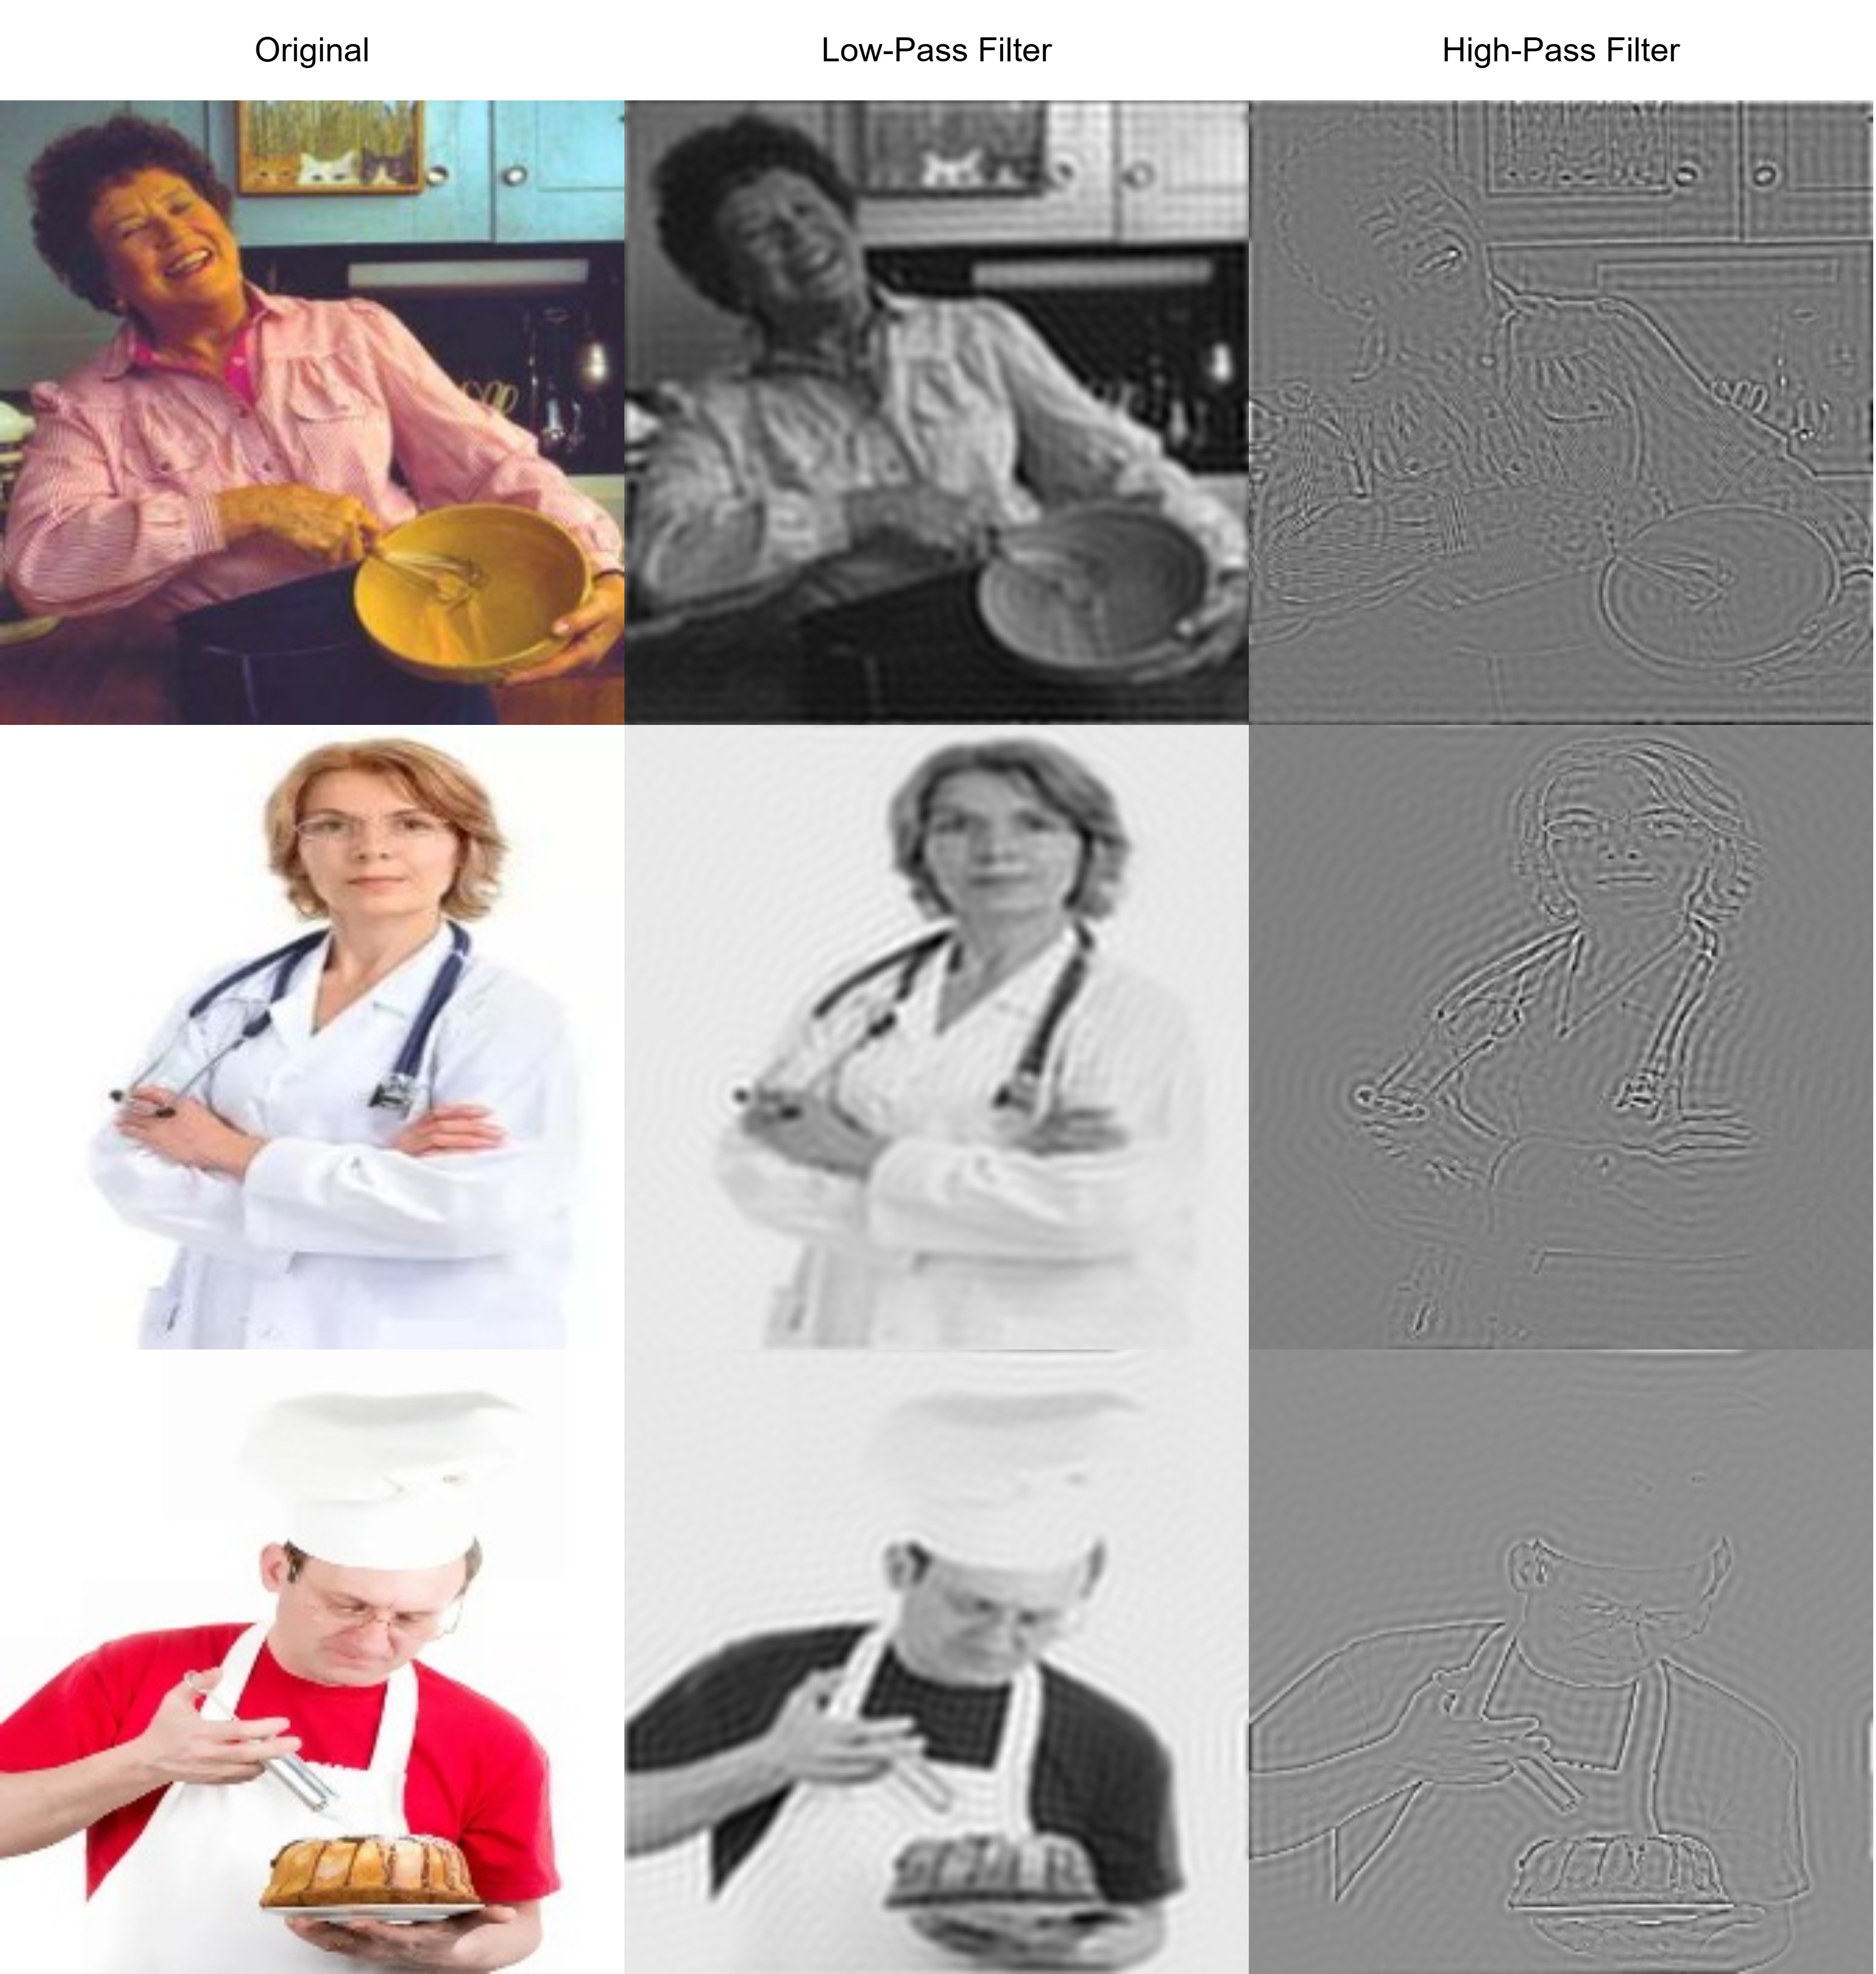
\includegraphics[width=\textwidth]{TD2.jpg}
	\caption{Frequency domain transformation outputs applied to three 
		profession-conditioned images. 
		\emph{Low-Pass Filter}: reconstruction from frequency components 
		within the circular cutoff radius $r = 40$, retaining smooth 
		global luminance and colour gradients while suppressing fine-grained 
		detail. 
		\emph{High-Pass Filter}: the complementary residual, isolating 
		fine textures, sharp edges, and compression artefacts. Both 
		representations are derived from a single FFT pass per image and 
		saved as greyscale PNGs.}
	\label{fig:td_frequency}
\end{figure}

\subsubsection{Pixel Shuffling, Patch Shuffling, and Mean RGB}

This subsection covers three related transformations that progressively 
reduce the spatial information available to a classifier, from complete 
spatial destruction through controlled local structure preservation to 
global colour summarisation. Together they form a spatial decomposition 
experiment that isolates the contribution of global composition, local 
structure, and colour statistics independently.

\paragraph{Pixel Shuffling}
Pixel shuffling randomly permutes the spatial position of every pixel in 
an image while preserving the overall colour distribution exactly. Each 
pixel is moved as an intact RGB triplet, ensuring that the joint colour 
distribution across channels is maintained while all spatial structure is 
destroyed. The resulting image retains no edges, textures, or object 
arrangements, reducing the available signal to global colour statistics 
alone. Zeng et al.\ \cite{Zeng_2024_UnderstandingBiasinLargeScaleVisualDatasets} 
report that pixel shuffling reduces classification accuracy from 82.0\% to 
52.2\% across the YCD datasets, just above the 33.3\% chance level for a 
three-class problem, confirming that colour statistics alone carry only 
modest discriminative signal and that spatial structure is the dominant axis 
of dataset bias.

Each image was resized to $224 \times 224$ pixels prior to transformation 
using bilinear interpolation. All pixels were then randomly permuted across 
spatial positions independently per image, with the permutation seed derived 
deterministically from the sum of the RGB channel values of the top-left 
pixel, ensuring reproducibility without requiring a global fixed seed that 
would produce identical permutations across images.

\paragraph{Patch Shuffling}
Patch shuffling generalises pixel shuffling by permuting fixed-size 
non-overlapping patches rather than individual pixels. Within each patch, 
spatial structure is fully preserved; only the arrangement of patches across 
the image is randomised. This transformation therefore tests the contribution 
of local spatial structure at a given scale: as patch size increases, more 
local context is preserved within each patch, and classification accuracy 
reflects the discriminative power of local texture and shape rather than 
global composition. Zeng et al.\ \cite{Zeng_2024_UnderstandingBiasinLargeScaleVisualDatasets} 
demonstrate that $16 \times 16$ patch shuffling recovers nearly all 
discriminability at 81.2\%, compared to 52.2\% for pixel shuffling, 
establishing that local spatial structure within small image regions is 
sufficient to distinguish datasets without any global compositional 
information.

Patch shuffling was applied at four scales: $2 \times 2$, $4 \times 4$, 
$8 \times 8$, and $16 \times 16$ pixels, spanning the range from 
near-pixel-level local structure to coarser spatial blocks and enabling the 
accuracy profile across patch sizes to be d rather than relying 
on a single scale. Each patch size constitutes an independent classification 
experiment. Images were resized to $224 \times 224$ pixels prior to 
transformation; as all four patch sizes divide 224 evenly, shuffling covers 
the full image without remainder. Patches were shuffled using a per-image 
deterministic seed derived from the sum of all pixel values in the first 
patch, consistent with the pixel shuffling procedure.

\paragraph{Mean RGB}
The mean RGB transformation compresses each image to a single average colour 
per channel, filling the entire image canvas with that uniform colour. All 
spatial, textural, and structural information is destroyed, leaving only the 
three-dimensional mean colour vector as the available signal. Zeng et al.\ 
\cite{Zeng_2024_UnderstandingBiasinLargeScaleVisualDatasets} report that even 
this extreme reduction achieves 48.5\% accuracy across the YCD datasets, 
approximately 15 percentage points above chance, confirming that global 
colour distributions carry a non-trivial spurious signal even in the complete 
absence of spatial information.

The mean RGB value was computed as the per-channel spatial mean across all 
pixels in the resized $224 \times 224$ image. The resulting three scalar 
values were used to fill a uniform-colour image of the same dimensions, saved 
as a standard three-channel PNG for classifier input. In addition to the 
filled image, the raw mean RGB vector and a channel-normalised equivalent 
— obtained by dividing each channel value by 255 to produce a unit-range 
vector in $[0, 1]$ — were recorded to a JSONL statistics file to support 
auxiliary linear probe experiments. Mean RGB also features in the demographic 
feature isolation experiments of 
\cite{Meister_2023_GenderArtifactsinVisualDatasets}, where it serves the 
distinct purpose of isolating colour as a carrier of gender-correlated signal, 
and is extended in this work to skin tone classification. In that context, the 
raw three-dimensional mean RGB vector is supplied directly as input to a 
logistic regression classifier rather than the filled uniform-colour image 
being passed to the ConvNeXt-Tiny network; the derivation procedure is 
otherwise identical in both contexts. Figure~\ref{fig:td_spatial} illustrates the three spatial decomposition transformations applied to representative images.

As with all preceding dataset classification transformations, the three-class 
configuration of Re-LAION-5B, Stable Diffusion v1.5 outputs, and COCO was 
used throughout, following the design described in Section~\ref{subsec:depth}. 
The combination of pixel shuffling, patch shuffling at four scales, and mean 
RGB provides a comprehensive spatial decomposition: the accuracy profile 
across these transformations characterises the scale at which local structure 
transitions from uninformative to discriminative, and quantifies the 
independent contribution of global colour statistics.

\begin{figure}[htbp]
	\centering
	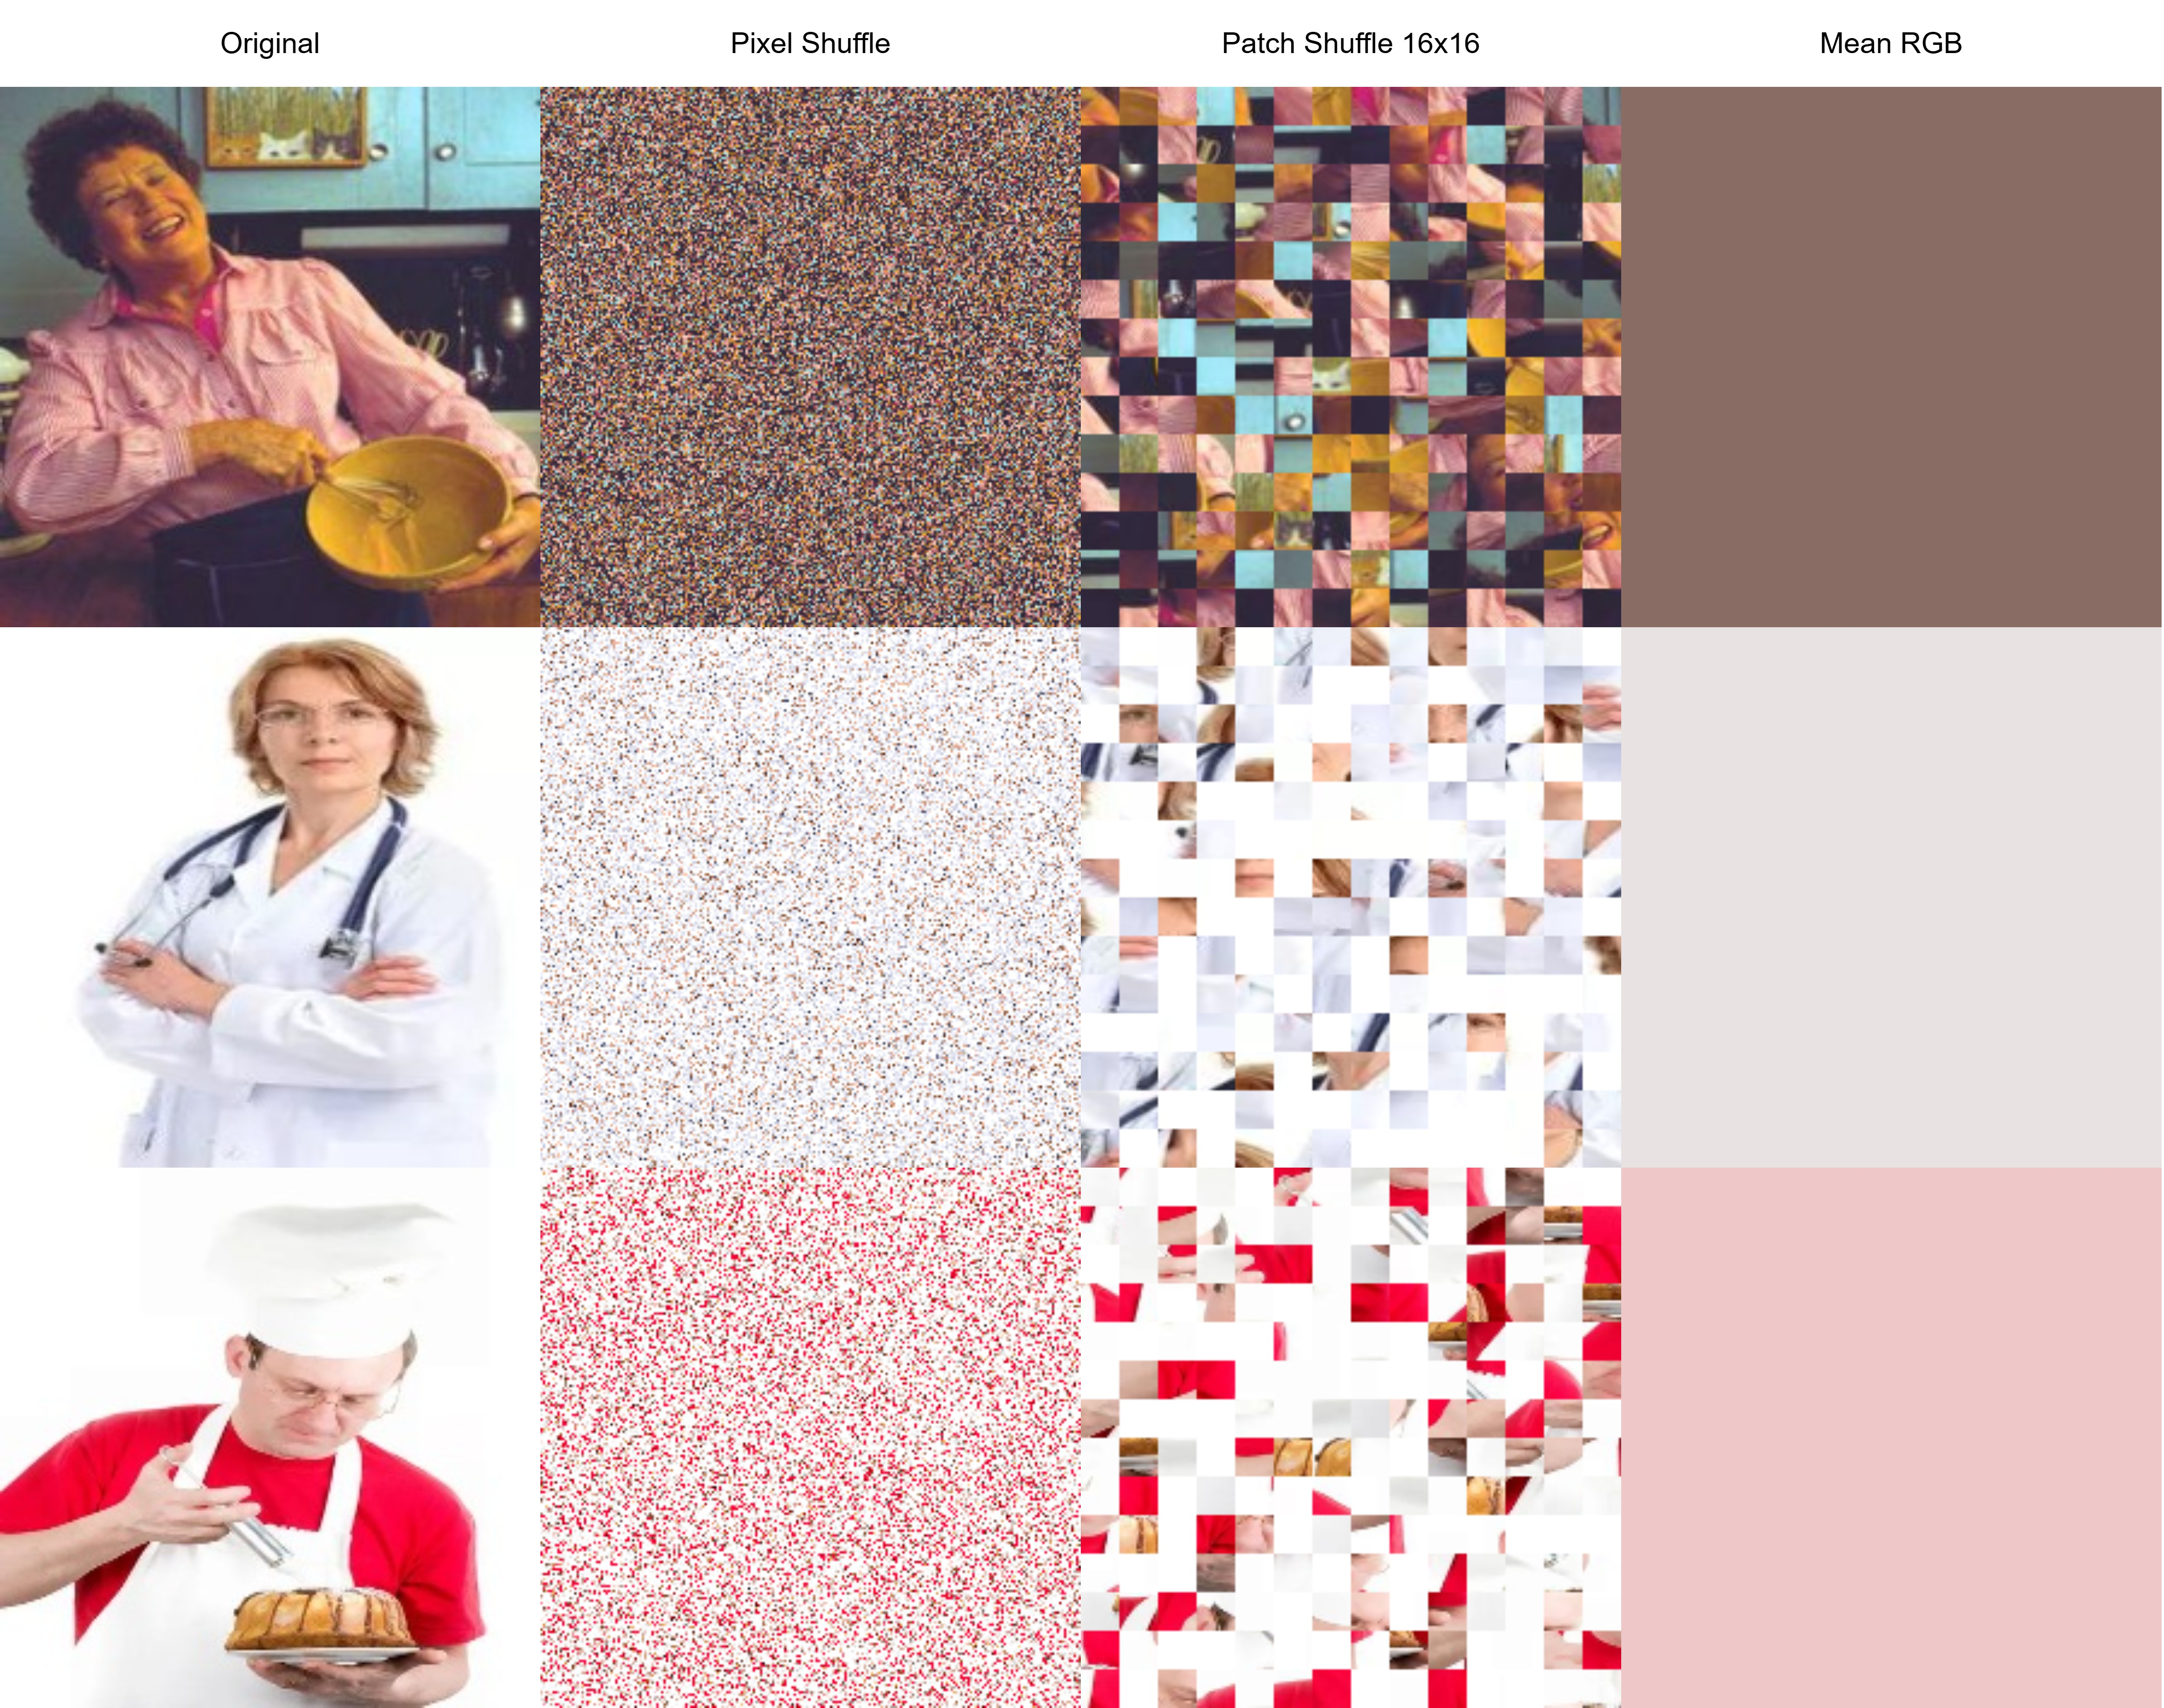
\includegraphics[width=\textwidth]{TD3.jpg}
	\caption{Spatial decomposition transformations applied to three 
		profession-conditioned images. 
		\emph{Pixel Shuffle}: all pixels randomly permuted, preserving 
		the global colour distribution while destroying all spatial 
		structure. 
		\emph{Patch Shuffle 16$\times$16}: non-overlapping $16 \times 16$ 
		pixel patches randomly permuted, preserving local texture within 
		each patch while disrupting global composition. 
		\emph{Mean RGB}: the entire image replaced by a uniform fill of 
		the per-channel spatial mean, retaining only the three-dimensional 
		global colour vector.}
	\label{fig:td_spatial}
\end{figure}

\subsubsection{Variational Autoencoder Reconstruction}

The VAE reconstruction transformation passes each image through the encoder 
and decoder of a pretrained Variational Autoencoder, producing a 
reconstructed image that has been compressed into and recovered from a 
low-dimensional latent representation. This bottleneck operation acts as a 
controlled lossy filter: fine-grained low-level properties such as JPEG 
compression artefacts, sensor noise, and resolution-specific texture detail 
are attenuated during compression, while semantically meaningful content 
and broad structural features are preserved in the reconstruction. As a 
spurious feature probe, VAE reconstruction therefore isolates whether 
dataset-discriminating signal survives latent compression — if it does, 
the bias resides primarily in semantic or structural content rather than 
in low-level acquisition artefacts. Zeng et al.\ 
\cite{Zeng_2024_UnderstandingBiasinLargeScaleVisualDatasets} report that 
VAE-reconstructed images achieve 77.4\% classification accuracy compared 
to the 82.0\% reference on unmodified images, a relatively modest reduction 
that confirms low-level properties such as compression artefacts and 
resolution differences contribute only marginally to the overall 
discriminative signal.

Reconstructions were produced using the KL-regularised autoencoder 
(\texttt{autoencoder\_kl\_64x64x3}) from the CompVis latent-diffusion 
repository \cite{Rombach_2022_CVPR}, the same VAE backbone used in the 
Stable Diffusion v1.5 architecture. Each image was resized to $256 \times 
256$ pixels using bicubic interpolation prior to encoding, matching the 
VAE's native operating resolution, and normalised to the range $[-1, 1]$ 
via the transformation $x \mapsto (x - 0.5) \times 2$ applied to the 
unit-range pixel values. The posterior mode was used for encoding rather 
than a stochastic sample (\texttt{sample\_posterior=False}), ensuring that 
reconstructions are deterministic and not subject to sampling variance 
across runs. The decoded output was rescaled from $[-1, 1]$ back to $[0, 1]$ 
via $y \mapsto (y / 2) + 0.5$ and clamped to $[0, 1]$ to enforce valid 
pixel range, then resized to $224 \times 224$ pixels via bicubic 
interpolation with \texttt{align\_corners=False} for compatibility with the 
ConvNeXt-Tiny classifier. Images therefore undergo two resize operations — 
bicubic interpolation to $256 \times 256$ prior to encoding and a second 
bicubic resize to $224 \times 224$ after decoding — with the VAE operating 
exclusively at its native resolution between the two. Example VAE reconstructions are shown in 
Figure~\ref{fig:td_semantic_latent}. Inference was 
performed in half-precision (FP16) under \texttt{torch.inference\_mode()} 
with mixed-precision autocast, and the model was compiled using 
\texttt{torch.compile} in \texttt{reduce-overhead} mode to maximise 
throughput.

A methodological consideration specific to this transformation concerns the 
relationship between the VAE and the Stable Diffusion v1.5 generated images. 
Because the VAE used for reconstruction is the same architecture and 
checkpoint embedded within Stable Diffusion v1.5, generated images are 
effectively being passed through the same decoder that produced them. This 
means that any latent-space artefacts introduced during generation are 
preserved through reconstruction with higher fidelity than would be expected 
for Re-LAION-5B or COCO images, for which the VAE constitutes a genuinely 
external compression step. This asymmetry should be considered when 
interpreting per-class classification accuracy on VAE-reconstructed images: 
higher separability for Stable Diffusion outputs may partially reflect this 
architectural proximity rather than solely the presence of spurious semantic 
features.

As with all preceding dataset classification transformations, the three-class 
configuration of Re-LAION-5B, Stable Diffusion v1.5 outputs, and COCO was 
used, following the design described in Section~\ref{subsec:depth}. High 
classification accuracy on VAE-reconstructed images would indicate that 
dataset-level bias is robust to latent compression and therefore unlikely 
to be eliminated by filtering pipelines that operate at the pixel level alone.

\subsubsection{Semantic Segmentation}
Semantic segmentation assigns a class label to every pixel in an image 
using a fixed category vocabulary, producing a colour-coded map that 
retains the spatial distribution of object categories while discarding 
all texture, colour, and fine-grained appearance information. As a 
spurious feature probe, segmentation maps isolate whether 
dataset-discriminating signal resides in which types of objects appear 
and where they are positioned in the scene, independently of how those 
objects look. Zeng et al.\ 
\cite{Zeng_2024_UnderstandingBiasinLargeScaleVisualDatasets} report that 
segmentation using the ADE20K vocabulary \cite{Zhou_2017_ADE20K} achieves 
69.8\% classification accuracy across the YCD datasets, confirming that 
the spatial distribution of semantic object categories constitutes a 
substantial axis of dataset-level bias. Notably, this accuracy is lower 
than that achieved by purely structural transformations such as depth 
estimation and edge detection, suggesting that object identity alone does 
not fully account for the discriminative signal captured by those 
representations.

Segmentation maps were produced using Mask2Former \cite{Cheng_2022_Mask2Former} 
with a Swin-Large backbone pretrained for semantic segmentation on ADE20K, 
accessed via the HuggingFace Transformers library 
(\texttt{facebook/mask2former-swin-large-ade-semantic}). Each image was 
resized to $512 \times 512$ pixels using bicubic interpolation prior to 
inference, matching the model's preferred input resolution. Segmentation 
was performed in half-precision (FP16) under \texttt{torch.no\_grad()} 
with mixed-precision autocast. The predicted per-pixel class index map 
was then resized to $224 \times 224$ pixels via nearest-neighbour 
interpolation, after which the standard ADE20K colour palette was applied 
to produce the final 150-class RGB segmentation map. Resizing the integer 
index map prior to palette application ensures that nearest-neighbour 
interpolation operates directly on discrete class labels, avoiding any 
corruption of class boundaries that would arise from interpolating RGB 
colour values. Images therefore undergo two resize operations — bicubic 
interpolation to $512 \times 512$ prior to inference and nearest-neighbour 
interpolation to $224 \times 224$ after segmentation — with the model 
operating exclusively at its native resolution between the two.

A methodological deviation from Zeng et al.\ concerns the segmentation 
backbone. The paper's implementation uses a Mask2Former model with a 
BEiTv2-ViT-Adapter-Large backbone trained at $896 \times 896$ resolution, 
which represents a substantially larger and more powerful architecture than 
the Swin-Large variant adopted here. The BEiTv2 variant was excluded on 
computational grounds: its dependency on the \texttt{mmsegmentation} and 
\texttt{ViT-Adapter} frameworks introduces complex installation 
requirements, and inference at $896 \times 896$ resolution with a 
ViT-Adapter-Large backbone is considerably more demanding than the 
HuggingFace Mask2Former pipeline. Both models use the same ADE20K 
vocabulary and produce semantically equivalent output representations; 
the primary difference is segmentation quality on ambiguous or 
fine-grained regions. Since the downstream classification task operates 
on the category distribution of the segmentation map rather than its 
pixel-level precision, the interpretive conclusions drawn from 
classification accuracy remain valid under the Swin-Large backbone, 
though absolute accuracy may differ slightly from the 69.8\% reported 
by Zeng et al.\ due to this architectural difference.

As with all preceding dataset classification transformations, the 
three-class configuration of Re-LAION-5B, Stable Diffusion v1.5 outputs, 
and COCO was used, following the design described in 
Section~\ref{subsec:depth}. High classification accuracy on segmentation 
maps would indicate that the three datasets differ systematically in the 
types and spatial arrangements of objects they contain, pointing to 
semantic co-occurrence patterns as a source of spurious signal that 
persists after all appearance information has been removed. Figure~\ref{fig:td_segmentation_occlusion} shows representative 
segmentation maps and segmentation-derived occlusion variants for 
three profession-conditioned images.

\begin{figure}[htbp]
	\centering
	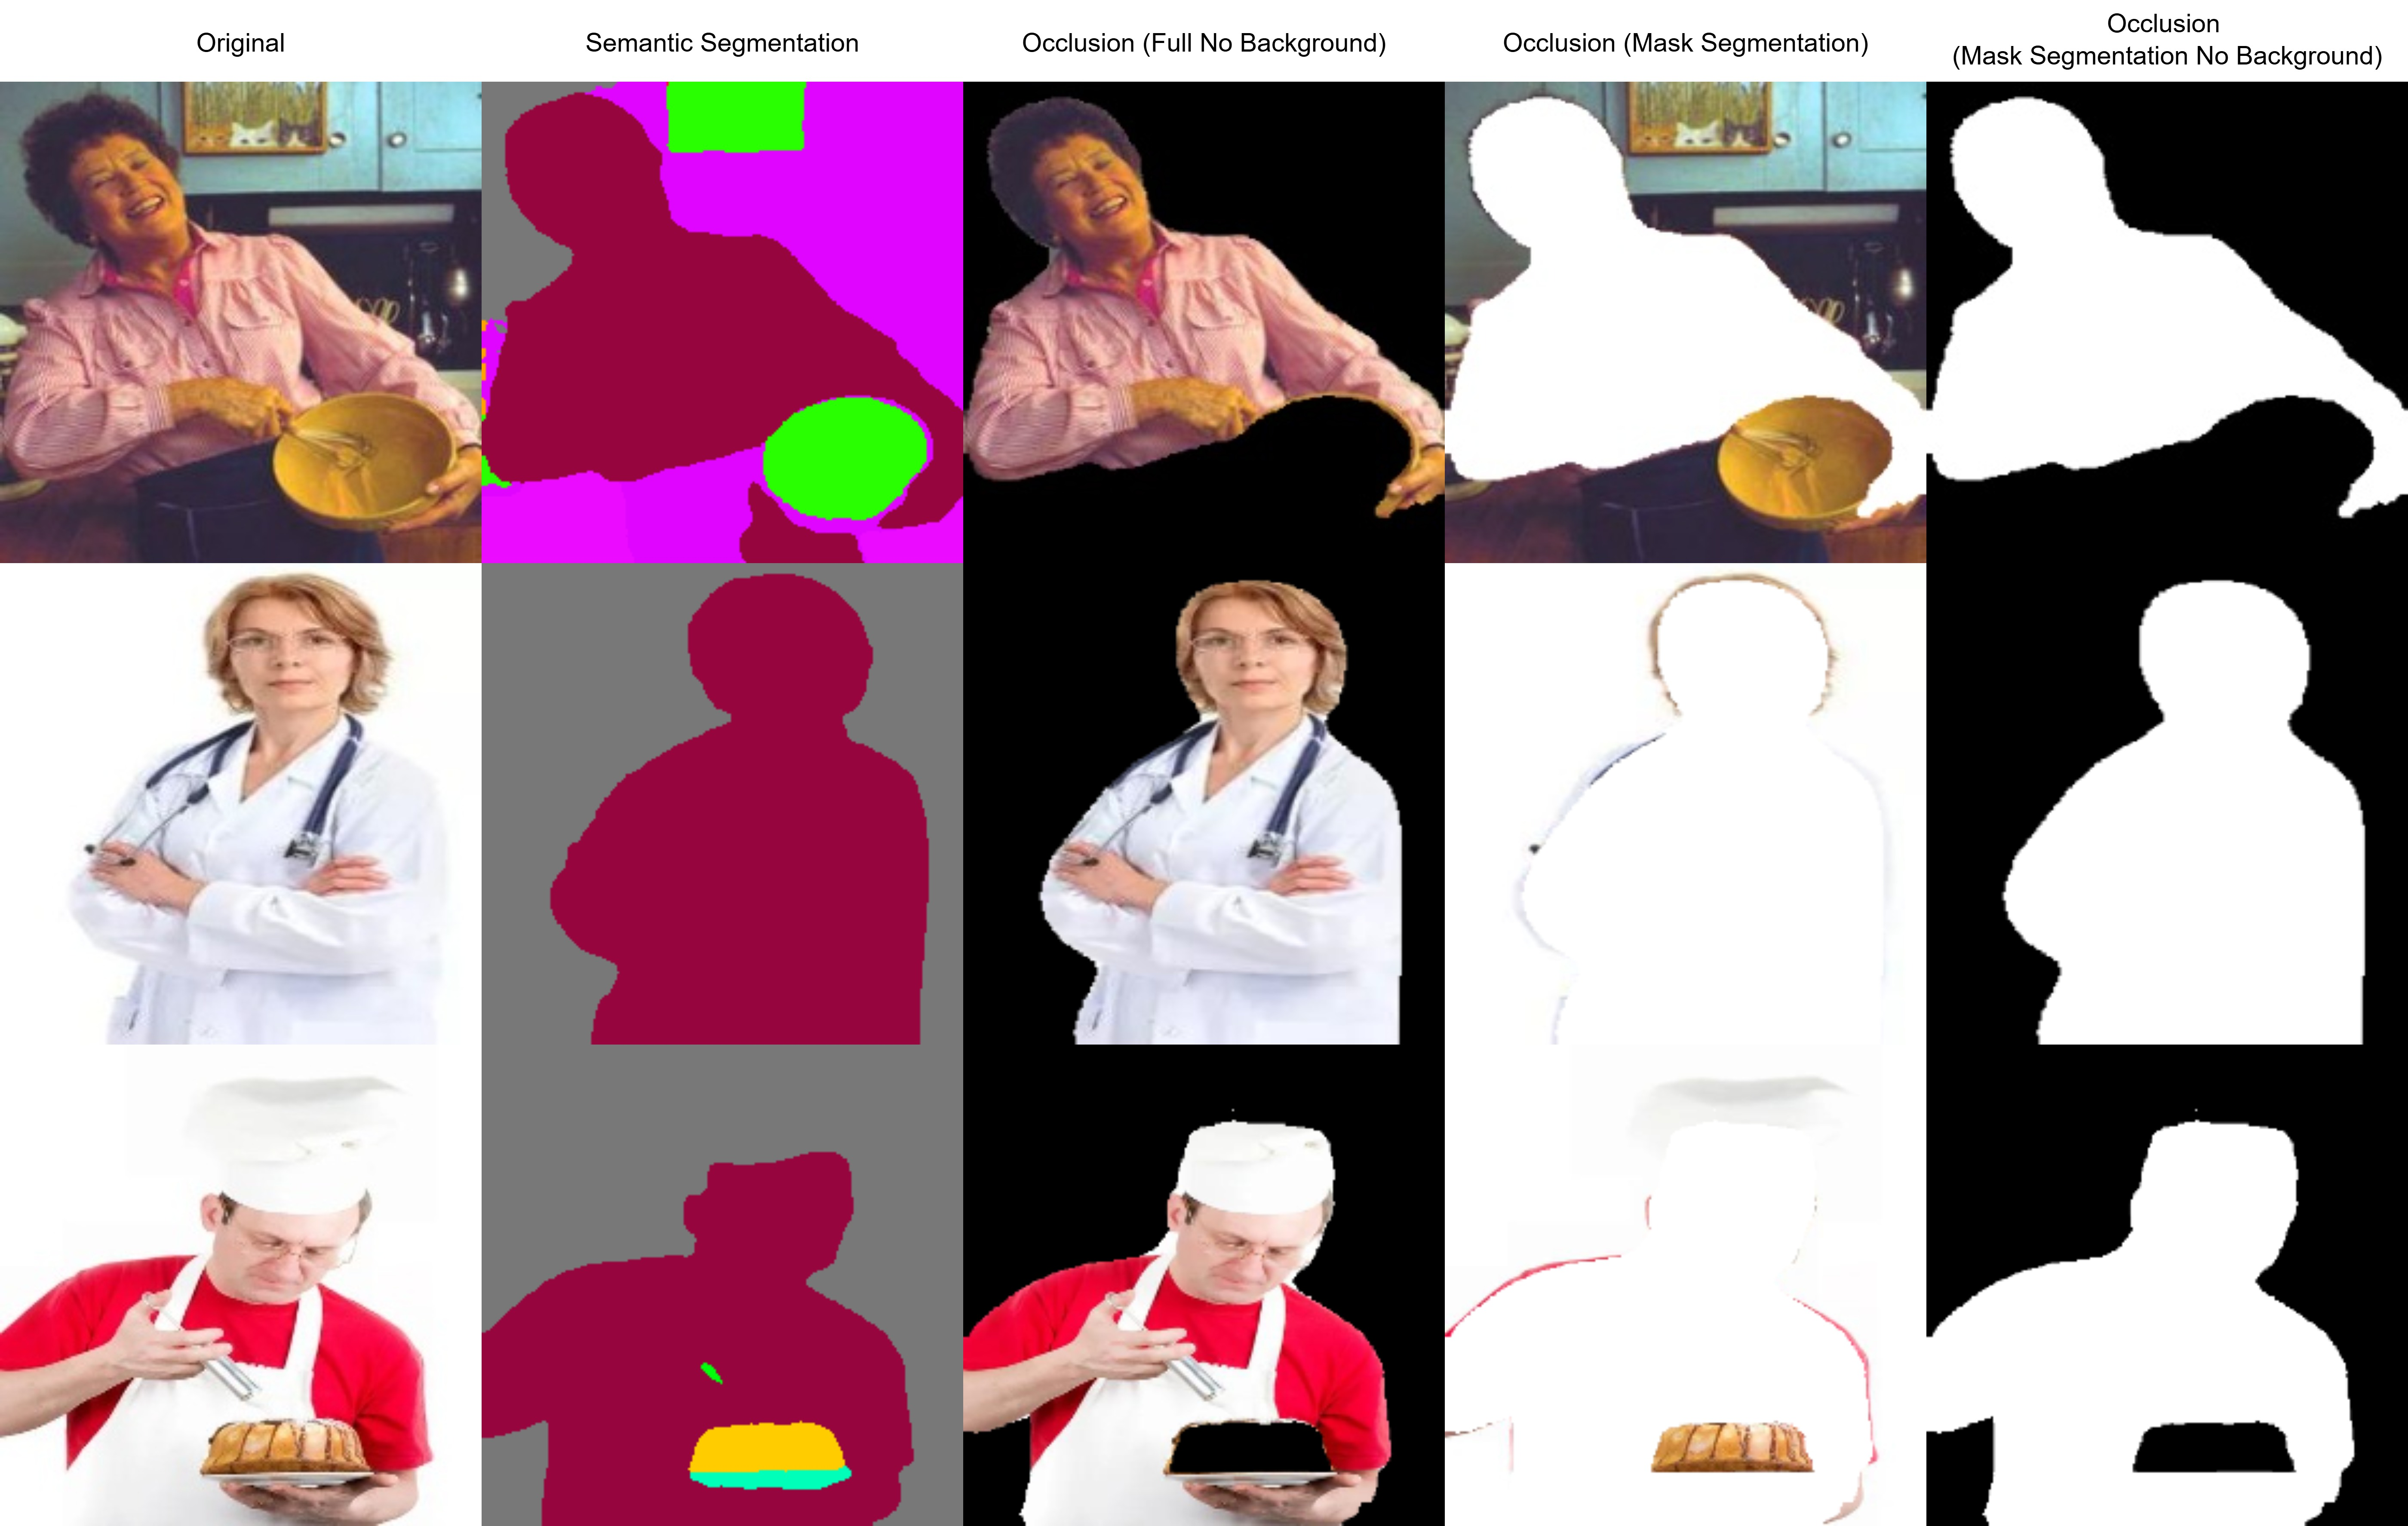
\includegraphics[width=\textwidth]{TD5.jpg}
	\caption{Semantic segmentation and segmentation-derived occlusion 
		representations applied to three profession-conditioned images. 
		\emph{Semantic Segmentation}: ADE20K colour-coded pixel-label map 
		produced by Mask2Former with a Swin-Large backbone, retaining 
		spatial object category distributions while discarding all texture 
		and colour. 
		\emph{Occlusion (Full No Background)}: the subject isolated from 
		the scene using the person segmentation mask, with all background 
		pixels zeroed. 
		\emph{Occlusion (Mask Segmentation)}: the person region replaced 
		by a uniform white fill derived from the segmentation mask, removing 
		the subject while preserving background context. 
		\emph{Occlusion (Mask Segmentation No Background)}: the person mask 
		only, rendered as a white silhouette on a black background.}
	\label{fig:td_segmentation_occlusion}
\end{figure}

\subsubsection{Object Detection}

Object detection reduces each image to a set of labelled bounding boxes, 
retaining object identity, approximate spatial location, and co-occurrence 
statistics while discarding all pixel-level appearance information including 
colour, texture, and internal object structure. As a spurious feature probe, 
object detection representations isolate whether dataset-discriminating signal 
resides in which objects appear in a scene and how they are spatially arranged, 
independently of how those objects look. Zeng et al.\ 
\cite{Zeng_2024_UnderstandingBiasinLargeScaleVisualDatasets} report that object 
detection achieves 61.9\% classification accuracy across the YCD datasets, lower 
than segmentation and structural transformations, suggesting that object identity 
and co-occurrence alone account for a smaller share of dataset-level bias than 
spatial geometry or semantic category distribution.

\paragraph{Object Vocabulary Selection}
Four candidate detection vocabularies were evaluated prior to model selection: 
COCO \cite{Lin_2014_COCO} (80 classes), OpenImages V7 
\cite{Kuznetsova_2020_OpenImagesV4} (601 classes), LVIS \cite{Gupta_2019_LVIS} 
(1{,}203 classes), and Object365 \cite{Shao_2019_Object365} (365 classes). COCO 
was excluded on the basis of insufficient vocabulary breadth: its 80 classes are 
too coarse to capture the range of occupation-relevant objects present in 
profession-conditioned imagery, particularly for equipment, tools, clothing, and 
workplace artefacts. LVIS was excluded as its 1{,}203 classes introduce a long 
tail of rare and fine-grained categories that add detection noise without 
improving interpretability at dataset scale, and detectors trained on LVIS are 
generally less reliable on common object categories due to the dataset's inherent 
class imbalance. Object365 was excluded as it offers intermediate coverage but 
lacks the breadth of occupation-relevant clothing and implement classes available 
in OpenImages V7. OpenImages V7 was selected as it provides a vocabulary of 601 
classes spanning a broad and balanced range of categories directly relevant to 
the professional contexts under analysis, including clothing, tools, medical 
equipment, musical instruments, and workplace implements.

\paragraph{Model Selection}
Eight detection models were evaluated on a 10{,}000-image subset of Re-LAION-5B 
at $640 \times 640$ pixel input resolution to assess practical feasibility at 
the scale of the full three-dataset corpus. Table~\ref{tab:objdet_speed} 
summarises inference times for each model evaluated.

\begin{table}[ht]
	\centering
	\caption{Object detection model inference time on a 10{,}000-image subset 
		of Re-LAION-5B at $640 \times 640$ pixel input resolution on a single GPU.}
	\label{tab:objdet_speed}
	\begin{tabular}{lll}
		\hline
		\textbf{Model} & \textbf{Time (10k images)} & \textbf{Architecture} \\
		\hline
		YOLOv8x (OIV7)              & $\sim$7 min 06 sec  & CNN, closed-vocabulary \\
		YOLOv8m (OIV7)              & $\sim$5 min 47 sec  & CNN, closed-vocabulary \\
		YOLOv8x-World               & $\sim$8 min 11 sec  & CNN, open-vocabulary \\
		YOLOv8x-Worldv2             & $\sim$7 min 23 sec  & CNN, open-vocabulary \\
		YOLOv8x + World (Ensemble)  & $\sim$12 min 44 sec & Ensemble \\
		RT-DETR-X                   & $\sim$6 min 24 sec  & Transformer, end-to-end \\
		GroundingDINO               & $>$60 min           & Vision-language model \\
		ViTDet-Huge                 & $>$60 min           & Transformer backbone \\
		\hline
	\end{tabular}
\end{table}

\textbf{ViTDet-Huge} \cite{Li_2022_ViTDet} is the model used in the original 
Zeng et al.\ implementation, employing a large-scale Vision Transformer backbone 
trained on the LVIS vocabulary. It was excluded from this work on two grounds: 
its inference time exceeded one hour on the 10{,}000-image subset, rendering it 
impractical at full dataset scale, and its reliance on the LVIS vocabulary 
conflicts with the OpenImages V7 vocabulary selected for this work. 
\textbf{GroundingDINO} \cite{Liu_2024_GroundingDINO} is an open-vocabulary 
vision-language model that achieved 52.5 AP on COCO in a zero-shot setting and 
set a record on the ODinW zero-shot benchmark. It was evaluated as a candidate 
for its prompt-based flexibility on large, weakly curated datasets, but its 
cross-modal attention mechanisms resulted in inference times exceeding one hour 
on the same subset, making it equally impractical. \textbf{RT-DETR-X} 
\cite{Zhao_2024_RTDETR} is a transformer-based end-to-end detector that 
eliminates the need for Non-Maximum Suppression and demonstrated inference 
speeds comparable to YOLOv8x. It was excluded because its available pretrained 
weights target COCO and Object365 rather than OpenImages V7; evaluating it on 
the OpenImages V7 vocabulary without retraining would conflate dataset mismatch 
with model performance.

\textbf{YOLOv8x-World} and \textbf{YOLOv8x-Worldv2} extend the standard 
YOLOv8 architecture to an open-vocabulary setting, enabling detection via 
textual prompts rather than a fixed class taxonomy. These models were evaluated 
for their ability to accept the OpenImages V7 class list as a textual prompt, 
allowing vocabulary flexibility without retraining. However, evaluation on the 
OpenImages V7 validation set revealed substantially degraded performance relative 
to the natively trained closed-vocabulary model, as shown in 
Table~\ref{tab:objdet_oiv7}. Both World variants exhibited low precision and 
unstable recall across the OpenImages V7 taxonomy, reflecting the limitations of 
prompt-based class specification for large, fine-grained vocabularies where class 
identity is better encoded by training supervision than by textual prompts.

\begin{table}[ht]
	\centering
	\caption{Detection performance on the OpenImages V7 validation set. 
		World variants were evaluated by prompting with the full OpenImages V7 
		class list rather than using natively trained weights.}
	\label{tab:objdet_oiv7}
	\begin{tabular}{lllll}
		\hline
		\textbf{Model} & \textbf{mAP@0.5} & \textbf{mAP@0.5:0.95} & 
		\textbf{Precision} & \textbf{Recall} \\
		\hline
		YOLOv8x (OIV7)     & 0.4345 & 0.3614 & 0.4786 & 0.4374 \\
		YOLOv8m (OIV7)     & 0.4094 & 0.3336 & 0.4791 & 0.4007 \\
		YOLOv8x-World      & 0.1370 & 0.1140 & 0.2044 & 0.2568 \\
		YOLOv8x-Worldv2    & 0.1403 & 0.1160 & 0.1847 & 0.2600 \\
		\hline
	\end{tabular}
\end{table}

An \textbf{ensemble} combining YOLOv8x and YOLOv8x-World was also explored on 
the hypothesis that the open-vocabulary model might compensate for missed 
detections in the closed-vocabulary model. In practice this did not materialise: 
the substantially weaker OpenImages V7 performance of the World variant 
introduced additional false positives and degraded precision rather than 
improving recall. Ensemble inference time was also nearly additive at 
approximately 12 minutes 44 seconds per 10{,}000 images, with no demonstrable 
empirical gain to justify the cost.

\textbf{YOLOv8x} with OpenImages V7 pretrained weights was selected as the 
detection backbone. It achieved the highest performance across all reported 
metrics on the OpenImages V7 validation set, with mAP@0.5:0.95 of 0.3614 and 
a precision-recall balance of 0.4786 and 0.4374 respectively, and offers 
practical throughput of approximately 26 images per second. \textbf{YOLOv8m} 
was considered as a faster alternative but was not adopted as the reduction of 
approximately 80 seconds per 10{,}000 images did not justify the corresponding 
reduction in detection accuracy.

\paragraph{Detection Pipeline}
Detection was performed at $640 \times 640$ pixel input resolution with a 
confidence threshold of 0.1 and an IoU threshold of 0.5. Test-time augmentation 
and class-agnostic NMS were disabled following hyperparameter evaluation. Twelve 
human body-part classes present in the OpenImages V7 vocabulary — 
\textit{Human arm}, \textit{Human body}, \textit{Human ear}, \textit{Human eye}, 
\textit{Human face}, \textit{Human foot}, \textit{Human hair}, \textit{Human 
	hand}, \textit{Human head}, \textit{Human leg}, \textit{Human mouth}, and 
\textit{Human nose} — were excluded from all outputs, as these detections carry 
person-level appearance information rather than object co-occurrence signal and 
would reintroduce the confound the transformation is designed to suppress.

Detected bounding boxes were rendered as overlays on a uniform white canvas, 
removing all pixel-level appearance information and retaining only object 
identity, spatial position, and bounding box geometry. Each box is drawn in a 
class-specific colour sourced from a fixed per-class colour map, providing a 
redundant visual encoding of class identity alongside the text label. Each label 
is rendered as \texttt{class: confidence} (e.g.\ \texttt{Person: 0.87}), meaning 
the classifier receives both categorical and confidence information as part of 
the visual input. All detection results were also saved to a JSONL file recording 
raw bounding box coordinates, class labels, and confidence scores for each image, 
supporting any downstream probing analyses that require structured detection 
output rather than rendered images. Final outputs were resized to $224 \times 
224$ pixels for compatibility with the ConvNeXt-Tiny classifier. Representative detection outputs on a white canvas are shown in Figure~\ref{fig:td_semantic_latent}.

\paragraph{Label Remapping}
A label remapping strategy was applied to normalise class name variants and 
reduce gender-correlated label noise in the detection output. Two remapping 
configurations were produced, summarised in Table~\ref{tab:label_remap}. The 
standard remapping consolidates gender-specific person labels — \textit{Man}, 
\textit{Woman}, \textit{Boy}, and \textit{Girl} — into a single \textit{Person} 
class, preventing the detector's own gender attributions from introducing a 
confound into the downstream classification task. The restricted remapping 
extends this by additionally consolidating clothing and accessory labels that 
carry gender-correlated associations in the OpenImages V7 taxonomy — such as 
\textit{Dress}, \textit{Brassiere}, \textit{High heels}, and \textit{Lipstick} 
— into generic counterparts such as \textit{Clothing}, \textit{Footwear}, 
\textit{Cosmetics}, and \textit{Fashion accessory}. This restricted 
configuration removes the signal that would otherwise arise from the detector 
having implicitly learned gender-associated object co-occurrences from its 
training data, enabling a cleaner test of whether dataset-discriminating signal 
persists once gender-correlated object vocabulary is suppressed. In both 
configurations, class exclusion filtering is applied to the post-remapped labels, 
ensuring that any class consolidated into a retained category is not 
inadvertently suppressed.

\begin{table}[ht]
	\centering
	\caption{Label remapping configurations applied during object detection. 
		The standard remap consolidates gendered person labels only. The 
		restricted remap additionally consolidates gender-associated clothing 
		and accessory labels into generic categories.}
	\label{tab:label_remap}
	\begin{tabular}{llll}
		\hline
		\textbf{Original Label} & \textbf{Standard Remap} & 
		\textbf{Restricted Remap} & \textbf{Category} \\
		\hline
		Man            & Person  & Person  & Person \\
		Woman          & Person  & Person  & Person \\
		Boy            & Person  & Person  & Person \\
		Girl           & Person  & Person  & Person \\
		\hline
		Dress          & ---     & Clothing & Clothing \\
		Skirt          & ---     & Clothing & Clothing \\
		Miniskirt      & ---     & Clothing & Clothing \\
		Brassiere      & ---     & Clothing & Clothing \\
		Suit           & ---     & Clothing & Clothing \\
		Coat           & ---     & Clothing & Clothing \\
		Jacket         & ---     & Clothing & Clothing \\
		Jeans          & ---     & Clothing & Clothing \\
		Shirt          & ---     & Clothing & Clothing \\
		Shorts         & ---     & Clothing & Clothing \\
		Trousers       & ---     & Clothing & Clothing \\
		Tie            & ---     & Clothing & Clothing \\
		Scarf          & ---     & Clothing & Clothing \\
		Belt           & ---     & Clothing & Clothing \\
		Hat            & ---     & Clothing & Clothing \\
		Sun hat        & ---     & Clothing & Clothing \\
		Cowboy hat     & ---     & Clothing & Clothing \\
		Fedora         & ---     & Clothing & Clothing \\
		Sombrero       & ---     & Clothing & Clothing \\
		\hline
		High heels     & ---     & Footwear & Footwear \\
		Sandal         & ---     & Footwear & Footwear \\
		Boot           & ---     & Footwear & Footwear \\
		Sock           & ---     & Footwear & Footwear \\
		\hline
		Lipstick       & ---     & Cosmetics & Cosmetics \\
		Face powder    & ---     & Cosmetics & Cosmetics \\
		\hline
		Perfume        & ---     & Personal care & Personal care \\
		Hair spray     & ---     & Personal care & Personal care \\
		\hline
		Earrings       & ---     & Fashion accessory & Fashion accessory \\
		Necklace       & ---     & Fashion accessory & Fashion accessory \\
		Tiara          & ---     & Fashion accessory & Fashion accessory \\
		Handbag        & ---     & Fashion accessory & Fashion accessory \\
		\hline
	\end{tabular}
\end{table}

As with all preceding dataset classification transformations, the three-class 
configuration of Re-LAION-5B, Stable Diffusion v1.5 outputs, and COCO was 
used, following the design described in Section~\ref{subsec:depth}. High 
classification accuracy on white-background object detection representations 
would indicate that the datasets differ systematically in their object 
co-occurrence statistics and spatial arrangements independently of 
appearance-level features, pointing to semantic object distributions as a 
consistent source of spurious signal.

\begin{figure}[htbp]
	\centering
	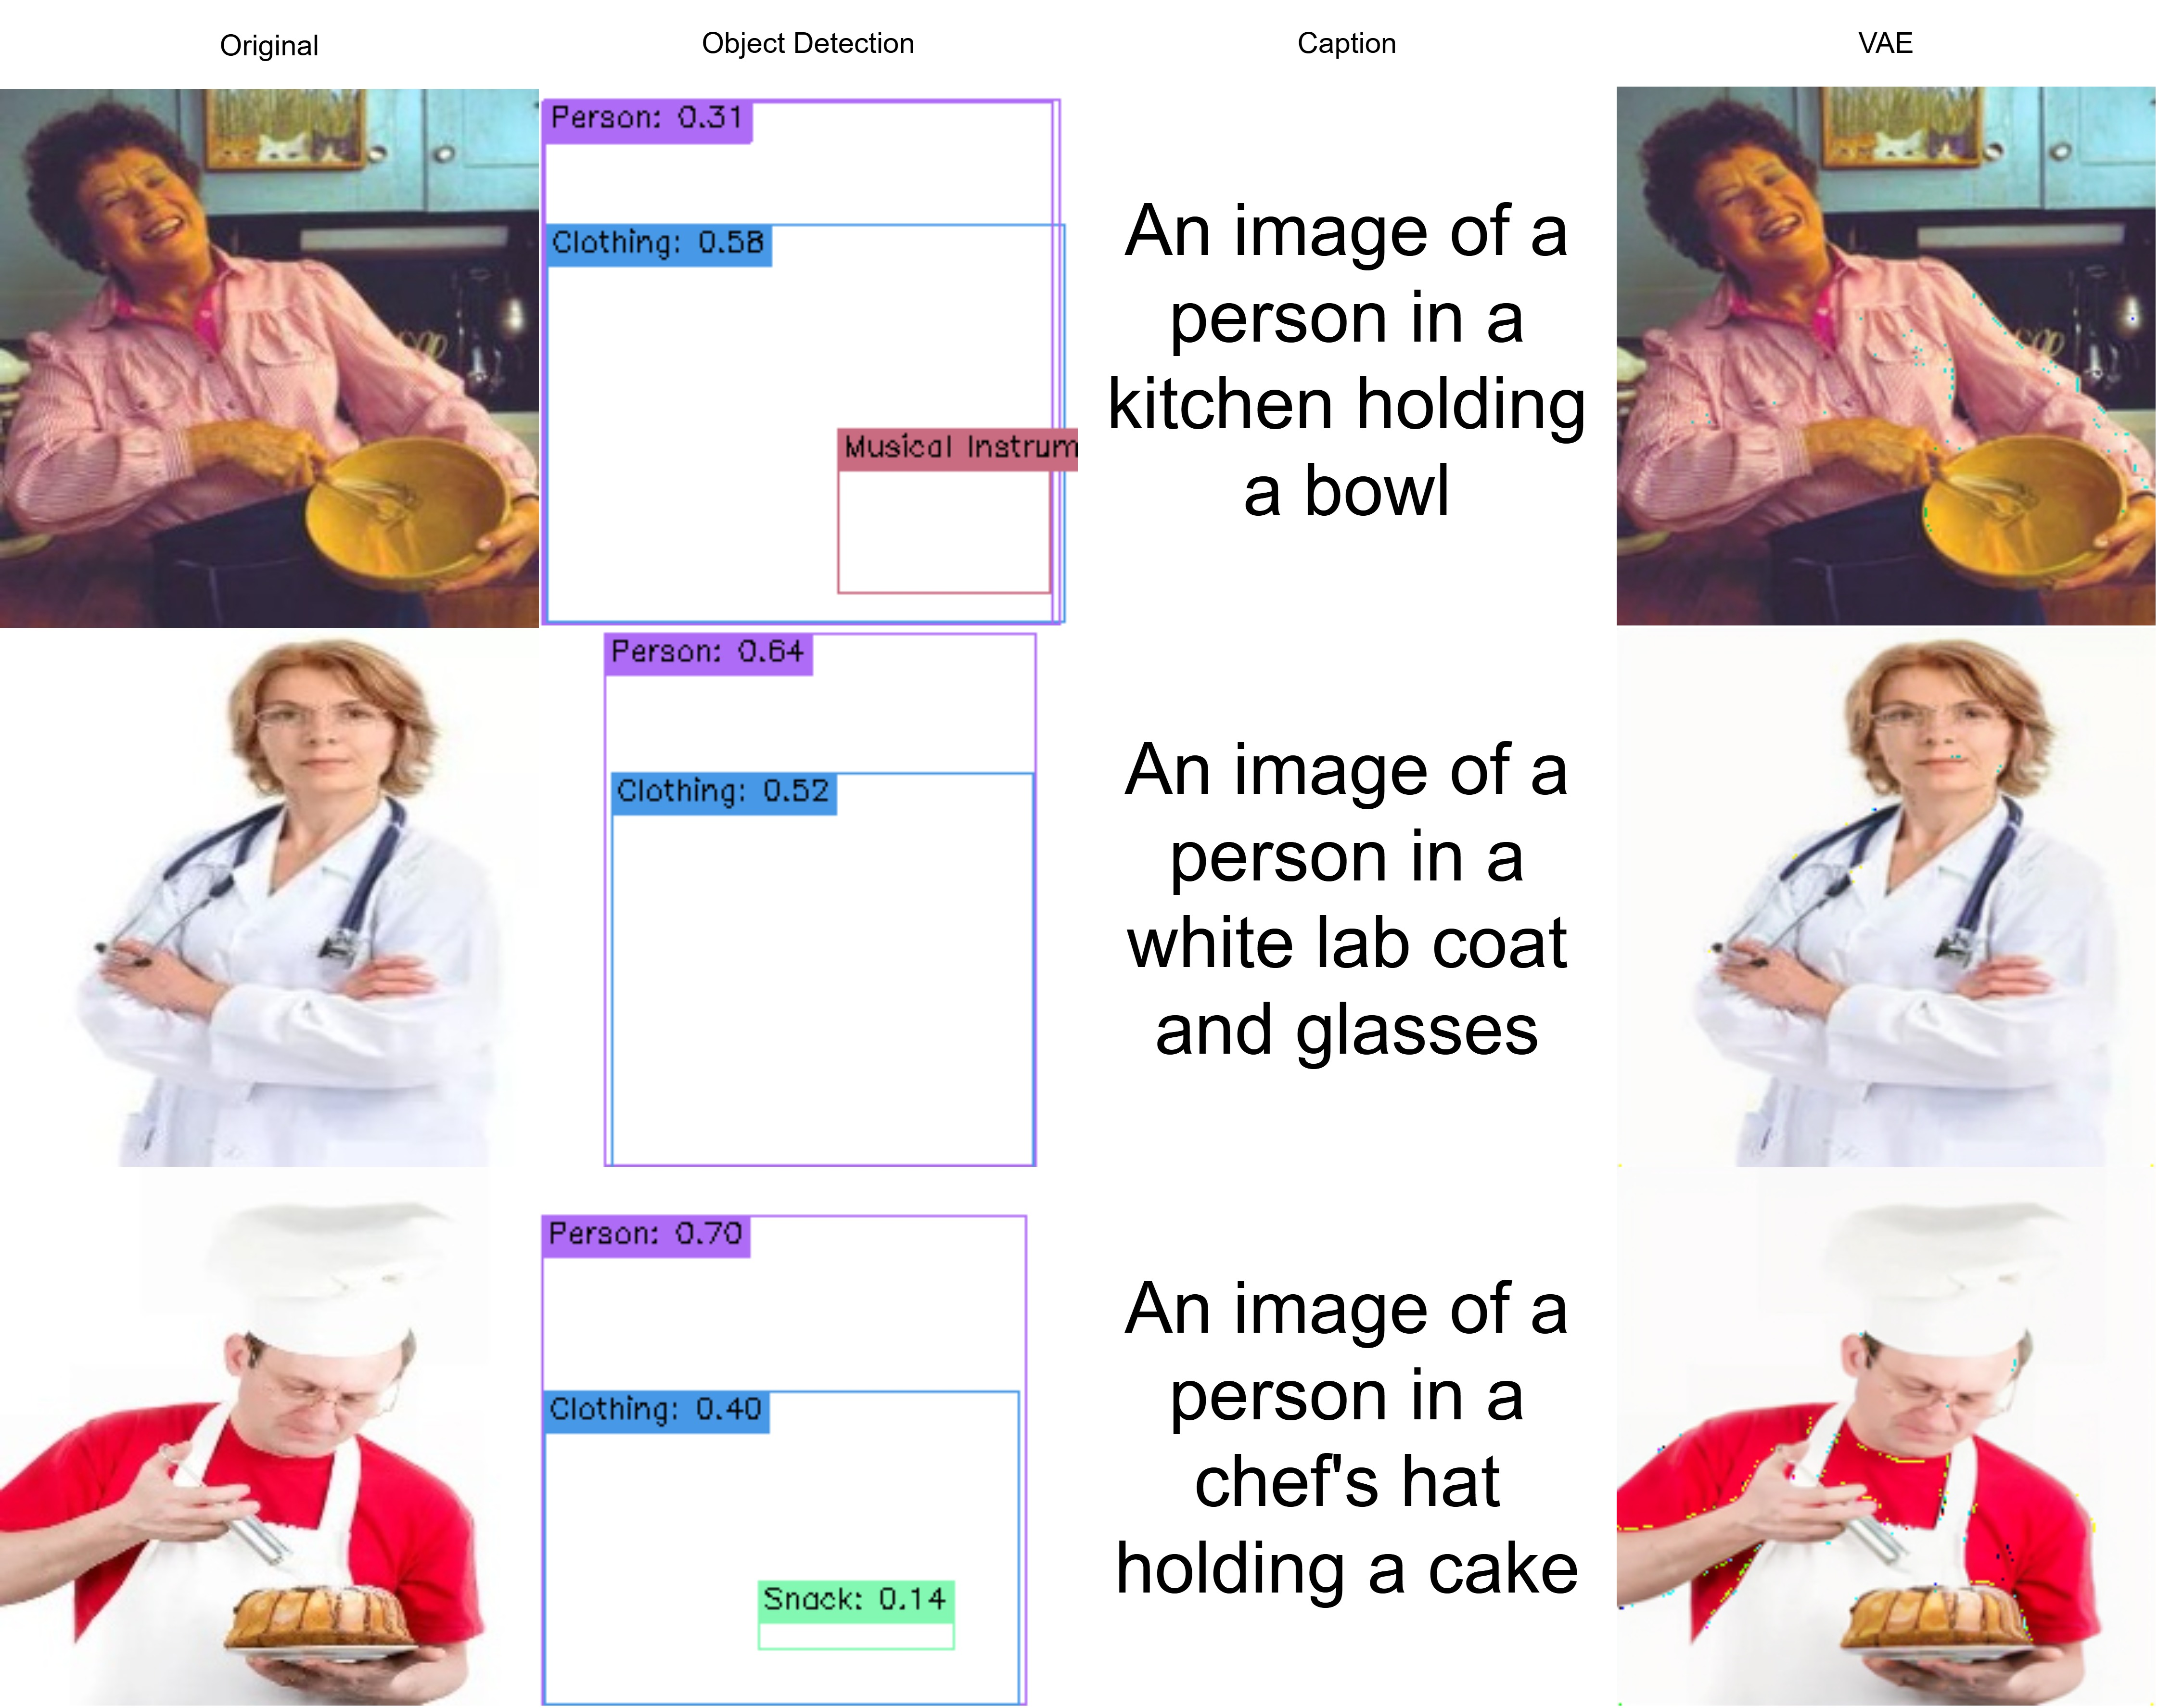
\includegraphics[width=\textwidth]{TD4.jpg}
	\caption{Semantic and latent-space transformation outputs applied to 
		three profession-conditioned images. 
		\emph{Object Detection}: bounding boxes rendered on a white canvas 
		using YOLOv8x with OpenImages V7 weights; all pixel-level 
		appearance is discarded and only object identity, spatial position, 
		and confidence scores are retained. 
		\emph{Caption}: short natural language descriptions generated by 
		BLIP Large using the \texttt{"An image of"} prefix, following 
		gender-neutral remapping. 
		\emph{VAE}: reconstructions produced by the KL-regularised 
		autoencoder of Stable Diffusion v1.5, compressing each image 
		through a low-dimensional latent bottleneck before decoding.}
	\label{fig:td_semantic_latent}
\end{figure}


\subsubsection{Image Captioning}

Image captioning converts each image into a natural language description, 
reducing the visual representation to semantic content expressible in text 
while discarding the underlying pixel representation. As a spurious feature probe, 
caption-based classification tests whether dataset-discriminating signal 
survives this extreme semantic compression: if a classifier operating on 
caption embeddings can reliably distinguish dataset origin, the bias must 
reside in systematic differences in scene content, object co-occurrence, 
or compositional conventions that are consistently captured in natural 
language descriptions. Zeng et al.\ 
\cite{Zeng_2024_UnderstandingBiasinLargeScaleVisualDatasets} report 
classification accuracies of 63.8\% for short captions and 66.1\% for 
long captions using LLaVA 1.5 7B \cite{Liu_2023_LLaVA}, confirming that 
semantic content carries moderate dataset-discriminating signal even after 
all visual information has been converted to text.

\paragraph{Model Selection}
The LLaVA 1.5 7B model used by Zeng et al.\ was the first candidate 
evaluated, as direct replication would have been preferable. Model 
selection proceeded in two stages: an initial throughput screen to 
identify computationally feasible candidates, followed by a caption 
quality evaluation across the surviving models.

Ten models were assessed for throughput viability, summarised in 
Table~\ref{tab:caption_viability}. LLaVA 1.5 7B, 
TinyLLaVA-Phi-2-SigLIP-3.1B, and LLaVA-OneVision-Qwen2-0.5B were all 
excluded due to prohibitive inference times stemming from their 
autoregressive generation requirements, which limit effective batch sizes 
to 2 regardless of GPU memory availability. BLIP2-Flan-T5-XL achieved 
the same throughput as BLIP Large under 8-bit quantisation but was 
excluded because the quantisation dependency introduced an unnecessary 
constraint without any speed advantage, and 4-bit quantisation caused 
incoherent output. Moondream2 was excluded as it does not support batched 
inference. The five remaining models — BLIP Large \cite{Li_2022_BLIP}, 
Florence 2 Base \cite{Xiao_2024_Florence2}, Kosmos 2 
\cite{Peng_2023_Kosmos2}, ViT-GPT2, and Tiny — satisfied throughput 
requirements and were advanced to quality evaluation.

\begin{table}[ht]
	\centering
	\caption{Image captioning model throughput assessment. Inference times 
		measured on a single GPU at the batch sizes shown.}
	\label{tab:caption_viability}
	\begin{tabular}{llll}
		\hline
		\textbf{Model} & \textbf{Batch Size} & \textbf{Time (25 images)} & 
		\textbf{Viable} \\
		\hline
		LLaVA 1.5 7B \cite{Liu_2023_LLaVA}      & 2  & $\sim$27.0s   & No \\
		TinyLLaVA-Phi-2-SigLIP-3.1B              & 2  & $\sim$180.0s  & No \\
		LLaVA-OneVision-Qwen2-0.5B               & 2  & $\sim$180.0s  & No \\
		BLIP2-Flan-T5-XL \cite{Li_2023_BLIP2}    & 25 & $\sim$2.3s    & No \\
		Moondream2                                & 1  & N/A           & No \\
		BLIP Large \cite{Li_2022_BLIP}           & 25 & $\sim$2.3s    & \textbf{Yes} \\
		Florence 2 Base \cite{Xiao_2024_Florence2}& 25 & $\sim$2.6s    & \textbf{Yes} \\
		Kosmos 2 \cite{Peng_2023_Kosmos2}        & 25 & $\sim$1.9s    & \textbf{Yes} \\
		ViT-GPT2                                  & 25 & $\sim$2.1s    & \textbf{Yes} \\
		Tiny                                      & 25 & $\sim$2.2s    & \textbf{Yes} \\
		\hline
	\end{tabular}
\end{table}

\paragraph{Quality Evaluation}
The five viable models were benchmarked for caption quality on the 
Karpathy test splits of COCO 2014 \cite{Lin_2014_COCO} and Flickr30k 
\cite{Young_2014_Flickr30k} using a comprehensive suite of metrics: 
BLEU@1--4 \cite{Papineni_2002_BLEU}, METEOR \cite{Banerjee_2005_METEOR}, 
CIDEr \cite{Vedantam_2015_CIDEr}, 4-gram diversity, SBERT semantic 
alignment \cite{Reimers_2019_SBERT} using the \texttt{all-MiniLM-L6-v2} 
encoder, CLIP-S, and RefCLIP-S \cite{Hessel_2021_CLIPScore} computed 
using \texttt{openai/clip-vit-large-patch14}. The results are summarised 
in Tables~\ref{tab:caption_quality_classical} and 
\ref{tab:caption_quality_clip}.

\begin{table}[ht]
	\centering
	\caption{Classical caption quality metrics on the Karpathy test 
		splits of COCO 2014 and Flickr30k. 4-gram diversity is the ratio 
		of unique 4-grams to total 4-grams across all generated captions; 
		low values indicate degenerate template-based generation.}
	\label{tab:caption_quality_classical}
	\begin{tabular}{llllllll}
		\hline
		\textbf{Model} & \textbf{Dataset} & \textbf{BLEU@4} & 
		\textbf{METEOR} & \textbf{CIDEr} & \textbf{4-gram Div.} & 
		\textbf{SBERT} \\
		\hline
		BLIP Large   & COCO      & \textbf{0.1278} & \textbf{0.2096} & \textbf{0.0325} & 0.3406 & \textbf{0.1158} \\
		ViT-GPT2     & COCO      & 0.1290          & 0.1918          & 0.0307          & 0.3246 & 0.0904 \\
		Tiny         & COCO      & 0.1270          & 0.1964          & 0.0367          & \underline{0.0547} & 0.0562 \\
		Kosmos 2     & COCO      & 0.0947          & 0.2014          & 0.0050          & 0.3334 & 0.1449 \\
		Florence 2   & COCO      & 0.0842          & 0.1754          & 0.0013          & 0.2978 & 0.1373 \\
		\hline
		BLIP Large   & Flickr30k & \textbf{0.1254} & \textbf{0.1934} & 0.0268          & 0.4554 & \textbf{0.0866} \\
		ViT-GPT2     & Flickr30k & 0.1306          & 0.1890          & \textbf{0.0306} & \textbf{0.4935} & 0.0682 \\
		Tiny         & Flickr30k & 0.1386          & 0.1915          & 0.0375          & \underline{0.1499} & 0.0479 \\
		Kosmos 2     & Flickr30k & 0.0992          & 0.2044          & 0.0051          & 0.4492 & 0.1079 \\
		Florence 2   & Flickr30k & 0.0855          & 0.1834          & 0.0011          & 0.4504 & 0.1194 \\
		\hline
	\end{tabular}
\end{table}

\begin{table}[ht]
	\centering
	\caption{CLIP-based caption quality metrics on the Karpathy test 
		splits of COCO 2014 and Flickr30k. CLIP-S measures 
		image-caption alignment scaled to $[0, 2.5]$; RefSim is the 
		maximum cosine similarity between a generated caption and all 
		reference captions for the same image; RefCLIP-S is the harmonic 
		mean of CLIP-S and RefSim.}
	\label{tab:caption_quality_clip}
	\begin{tabular}{lllll}
		\hline
		\textbf{Model} & \textbf{Dataset} & \textbf{CLIP-S} & 
		\textbf{RefSim} & \textbf{RefCLIP-S} \\
		\hline
		BLIP Large   & COCO      & \textbf{0.6646} & 0.8148          & \textbf{0.7279} \\
		ViT-GPT2     & COCO      & 0.6040          & \textbf{0.8289} & 0.6951 \\
		Tiny         & COCO      & 0.4110          & 0.6087          & 0.4853 \\
		Kosmos 2     & COCO      & 0.5568          & 0.6314          & 0.5861 \\
		Florence 2   & COCO      & 0.5927          & 0.6536          & 0.6163 \\
		\hline
		BLIP Large   & Flickr30k & \textbf{0.6550} & 0.7330          & \textbf{0.6868} \\
		ViT-GPT2     & Flickr30k & 0.5290          & 0.6713          & 0.5867 \\
		Tiny         & Flickr30k & 0.4777          & 0.6371          & 0.5409 \\
		Kosmos 2     & Flickr30k & 0.5600          & 0.5766          & 0.5619 \\
		Florence 2   & Flickr30k & 0.6059          & 0.5759          & 0.5853 \\
		\hline
	\end{tabular}
\end{table}

BLIP Large achieved the highest scores across the most diagnostic metrics 
on both evaluation datasets. Its CLIP-S scores of 0.6646 on COCO and 
0.6550 on Flickr30k indicate strong visual grounding, while its RefCLIP-S 
scores of 0.7279 and 0.6868 are the highest across all five candidates on 
both datasets, confirming that its captions are simultaneously well-aligned 
with image content and semantically coherent relative to human references. 
BLIP Large also achieves the highest METEOR and SBERT scores on both 
datasets, both of which correlate more reliably with human judgement than 
BLEU due to their handling of synonyms and paraphrase. Florence 2 and 
Kosmos 2 were excluded despite acceptable throughput: both exhibit 
substantially lower CLIP-S and RefCLIP-S scores than BLIP Large, and 
their CIDEr scores are near zero on both datasets, indicating that their 
captions share little n-gram overlap with the reference distribution. 
ViT-GPT2 achieves competitive BLEU and higher RefSim than BLIP Large on 
COCO, but its CLIP-S and RefCLIP-S scores are consistently lower, 
indicating weaker image-caption alignment. A critical failure mode was 
identified in the Tiny model, which achieved a 4-gram diversity of only 
0.0547 on COCO — indicating that fewer than 6\% of all 4-grams across 
generated captions were unique, a hallmark of degenerate template-based 
generation. This finding demonstrates that traditional n-gram metrics such 
as BLEU are insufficient to identify caption quality failures and motivates 
the inclusion of diversity metrics in the evaluation protocol.

\paragraph{Gender-Neutral Remapping}
A word-level remapping was applied to all generated captions prior to 
saving, using case-insensitive whole-word matching with plural form 
support. The mapping neutralises gendered person references and gendered 
pronouns, replacing \textit{woman} and \textit{man} with \textit{person}, 
\textit{boy} and \textit{girl} with \textit{child}, and gendered pronouns 
(\textit{he}, \textit{she}, \textit{his}, \textit{her}, \textit{himself}, 
\textit{herself}) with their gender-neutral equivalents (\textit{they}, 
\textit{their}, \textit{themselves}). This remapping ensures that any 
downstream classifier operating on caption features cannot exploit gendered 
language introduced by the captioning model itself as a proxy for dataset 
origin, which would confound the attribution of classification signal to 
genuine semantic content differences between datasets.


Captions were generated using the prompt \texttt{"An image of"}, following 
the captioning evaluation protocol of Peng et 
al.\ \cite{Peng_2023_Kosmos2}, who adopt this prefix for image captioning 
on the Flickr30k Karpathy split. BLIP Large supports conditional caption 
generation in which the image-grounded text decoder continues from a 
supplied text prefix \cite{Li_2022_BLIP}; providing \texttt{"An image of"} 
as a prefix anchors generation into a descriptive register while imposing 
no domain-specific vocabulary, and ensures that captions from all evaluated 
models share a consistent conditional framing, removing prompt format as a 
potential confound in downstream classifier comparisons. A maximum output 
length of 30 tokens and greedy decoding (\texttt{num\_beams=1}, 
\texttt{do\_sample=False}) were used, producing short factual descriptions 
consistent in style with the short captions reported by Zeng et al. Inference was performed in half-precision (FP16) under \texttt{torch.no\_grad()}, with the model compiled using 
\texttt{torch.compile} in \texttt{reduce-overhead} mode to maximise 
throughput. Both raw and remapped caption variants were saved to a JSONL 
file per dataset to support sensitivity analysis. As with all preceding 
dataset classification transformations, the three-class configuration of 
Re-LAION-5B, Stable Diffusion v1.5 outputs, and COCO was used, following 
the design described in Section~\ref{subsec:depth}. Representative captions generated by BLIP Large are shown alongside object detection and VAE outputs in Figure~\ref{fig:td_semantic_latent}.


\subsubsection{Pose Estimation}
\label{subsec:pose}

Pose estimation reduces each image to a set of COCO-17 body joint 
coordinates, retaining only skeletal geometry --- joint positions, limb 
orientations, and body proportions --- while discarding all pixel-level 
appearance information including colour, texture, and facial structure. As 
a spurious feature probe following Meister et 
al.\ \cite{Meister_2023_GenderArtifactsinVisualDatasets}, pose 
representations isolate whether demographic attributes can be inferred from 
body geometry alone, independently of visual appearance cues. Unlike the 
preceding transformations, which produce rendered image outputs consumed by 
the ConvNeXt-Tiny classifier, the pose pipeline produces 34-dimensional 
normalised keypoint vectors that serve as direct input to a low-capacity 
Multi-Layer Perceptron (MLP) probe. This distinction reflects the 
fundamentally different nature of the representation: a fixed-length 
geometry vector has no spatial structure that a convolutional classifier 
could exploit, and the MLP's limited capacity ensures that any 
above-chance classification accuracy reflects genuine geometric signal 
rather than model expressiveness.

This transformation is applied exclusively to Re-LAION-5B and Stable 
Diffusion v1.5 image sets, which are conditioned on occupation-specific 
queries and therefore populated with images depicting people. COCO images 
are not guaranteed to contain people in the occupational contexts under 
analysis, and pose estimation applied to images without clearly visible 
subjects produces uninformative zero vectors that would contaminate the 
feature space rather than contribute meaningful signal. The pose 
transformation therefore operates as a two-dataset feature extraction step 
rather than a three-class classification transformation.

\paragraph{Model Selection}
Seventeen model configurations across five architectures were evaluated on 
all person-annotated images in the COCO 2017 validation set 
\cite{Lin_2014_COCO} to identify the best trade-off between keypoint 
localisation accuracy and throughput at the scale of the full image corpus. 
Evaluation followed the standard COCO keypoint evaluation protocol, 
reporting average precision at IoU thresholds of 0.5 and 0.5:0.95 
(AP, AP$_{50}$, AP$_{75}$), average recall (AR), frames per second (FPS), 
and image-level detection rate. Table~\ref{tab:pose_model_eval} summarises 
all results.

\begin{table}[ht]
	\centering
	\caption{Pose estimation model evaluation on all person-annotated 
		images in the COCO 2017 validation set. Standard mode uses the 
		model's integrated person detector. Oracle mode provides 
		ground-truth person bounding boxes directly to the keypoint 
		estimator, establishing an upper bound independent of detection 
		quality. FPS is measured end-to-end on a single GPU including 
		person detection where applicable.}
	\label{tab:pose_model_eval}
	\begin{tabular}{llllll}
		\hline
		\textbf{Model} & \textbf{AP} & \textbf{AP$_{50}$} & 
		\textbf{AP$_{75}$} & \textbf{AR} & \textbf{FPS} \\
		\hline
		\multicolumn{6}{l}{\textit{YOLOv8 (integrated detection + 
				keypoints)}} \\
		YOLOv8n-Pose          & 0.479 & 0.744 & 0.520 & 0.538 & 27.0 \\
		YOLOv8s-Pose          & 0.581 & 0.830 & 0.642 & 0.638 & 37.1 \\
		YOLOv8m-Pose          & 0.633 & 0.860 & 0.704 & 0.691 & 33.0 \\
		\textbf{YOLOv8l-Pose} & \textbf{0.659} & \textbf{0.871} & 
		\textbf{0.735} & \textbf{0.717} & \textbf{39.7} \\
		YOLOv8x-Pose          & 0.674 & 0.871 & 0.747 & 0.730 & 27.9 \\
		\hline
		\multicolumn{6}{l}{\textit{MoveNet (requires external person 
				detector)}} \\
		MoveNet-Lightning (Standard) & 0.419 & 0.621 & 0.456 & 0.450 & 9.9 \\
		MoveNet-Lightning (Oracle)   & 0.474 & 0.729 & 0.506 & 0.510 & 10.4 \\
		MoveNet-Thunder (Standard)   & 0.481 & 0.653 & 0.523 & 0.510 & 4.6 \\
		MoveNet-Thunder (Oracle)     & 0.548 & 0.779 & 0.594 & 0.584 & 4.1 \\
		\hline
		\multicolumn{6}{l}{\textit{MediaPipe (requires external person 
				detector)}} \\
		MediaPipe-C2 (Standard)      & 0.243 & 0.405 & 0.255 & 0.333 & 3.6 \\
		MediaPipe-C2 (Oracle)        & 0.238 & 0.393 & 0.251 & 0.334 & 4.3 \\
		\hline
		\multicolumn{6}{l}{\textit{HRNet (requires external person 
				detector)}} \\
		HRNet-W32 (Standard)         & 0.714 & 0.879 & 0.789 & 0.769 & 8.7 \\
		HRNet-W32 (Oracle)           & 0.766 & 0.933 & 0.842 & 0.798 & 10.4 \\
		HRNet-W32-384 (Standard)     & 0.727 & 0.880 & 0.794 & 0.781 & 7.2 \\
		HRNet-W32-384 (Oracle)       & 0.776 & 0.933 & 0.853 & 0.808 & 8.5 \\
		HRNet-W48 (Standard)         & 0.723 & 0.880 & 0.793 & 0.778 & 7.9 \\
		HRNet-W48 (Oracle)           & 0.773 & 0.934 & 0.852 & 0.806 & 8.4 \\
		\hline
	\end{tabular}
\end{table}

The evaluated architectures fall into two categories based on their person 
detection requirements. \textbf{YOLOv8-Pose} models integrate person 
detection and keypoint estimation in a single end-to-end forward pass, 
making them self-contained pipelines with no external dependency. The 
remaining architectures --- \textbf{MoveNet} 
\cite{Bazarevsky_2020_MoveNet}, \textbf{MediaPipe} 
\cite{Lugaresi_2019_MediaPipe}, and \textbf{HRNet} 
\cite{Wang_2020_HRNet} --- are top-down models that require an external 
person detector to crop each subject before keypoint estimation. For these 
models, evaluation was conducted in two modes: Standard mode, in which a 
YOLOv8-based person detector was used to supply crops; and Oracle mode, in 
which ground-truth COCO bounding boxes were provided directly to the 
keypoint estimator. Oracle results therefore represent accuracy upper bounds 
under perfect detection rather than realistic deployment performance.

MoveNet and MediaPipe were excluded on accuracy grounds. All MoveNet 
variants achieved AP below 0.55 even in Oracle mode. MediaPipe-C2 reached 
only 0.243 AP in Standard mode, with Oracle mode producing no improvement 
--- a result consistent with the model's architecture being optimised for 
real-time single-person inference rather than COCO-style multi-person 
evaluation, such that substituting ground-truth crops for its internal 
detection mechanism does not benefit localisation accuracy.

HRNet variants achieved the highest AP values across all evaluated models, 
with HRNet-W32-384 (Oracle) reaching 0.776 AP and a corresponding AR of 
0.808. However, all HRNet Standard configurations operate at under 9 FPS 
end-to-end, a rate that would render full-corpus extraction prohibitively 
slow. Furthermore, Standard mode HRNet performance is contingent on the 
quality of the upstream person detector, introducing a two-stage dependency 
that complicates reproducibility and error attribution.

YOLOv8x-Pose achieved the highest AP among the self-contained YOLOv8 
models at 0.674 with AR of 0.730, but at 27.9 FPS it is slower than 
YOLOv8l-Pose despite the marginal accuracy advantage of 0.015 AP. 
\textbf{YOLOv8l-Pose} was selected as the pose estimator on the basis of 
its superior throughput of 39.7 FPS --- the highest of any evaluated model 
--- combined with an AP of 0.659, AR of 0.717, and the practical advantage 
of requiring no external person detector. The accuracy gap relative to 
YOLOv8x-Pose is small and does not affect the downstream representational 
objective: since the pipeline discards all appearance information and 
retains only normalised joint geometry, moderate differences in keypoint 
localisation precision are less consequential than they would be in a 
predictive application.

\paragraph{Pose Extraction Pipeline}
For each image, YOLOv8l-Pose was applied at the native image resolution 
with a person detection confidence threshold of 0.25. When multiple person 
detections were returned, the detection with the highest box confidence 
score was retained and all others discarded, enforcing a single-person 
constraint per image consistent with the probing protocol of Meister et 
al.\ \cite{Meister_2023_GenderArtifactsinVisualDatasets}. Images in which 
no person was detected were encoded as all-zero pose vectors.

YOLO keypoint confidence values were converted to COCO-style visibility 
flags: joints with confidence at or above 0.5 were assigned visibility 
$v = 2$ (visible and reliable) and retained at their predicted coordinates; 
joints below this threshold were zeroed and assigned $v = 0$ (not 
labelled). This visibility masking suppresses unreliable low-confidence 
joints and ensures that missing joints are treated identically to 
unannotated keypoints in COCO ground truth.

Pose geometry was normalised to remove absolute scale and image position 
cues. For the raw keypoint representation, visible joints were identified 
as those whose coordinates are non-zero; for the visibility-annotated 
representation, visible joints were identified by their assigned $v > 0$ 
flag. In both cases, visible joints were centred by subtracting the mean 
joint position, and the bounding box area of visible joints was scaled to a 
fixed target area of 4{,}000 pixels, following the normalisation procedure 
of Meister et al.\ \cite{Meister_2023_GenderArtifactsinVisualDatasets}. 
Invisible joints remained at the origin after normalisation. This 
normalisation removes absolute image position, person scale, and 
camera-distance cues, leaving only relative joint geometry as the 
representational signal.

Each image produced a JSONL record containing four representations: raw 
keypoint coordinates (34-dimensional flat vector), keypoints with COCO 
visibility flags (51-dimensional), and normalised equivalents of each. The 
34-dimensional normalised keypoint vector, which retains geometry while 
discarding both appearance and visibility metadata, serves as direct input 
to the downstream MLP probe. All vectors follow strict COCO-17 joint 
ordering. Figure~\ref{fig:td_structural_transforms} shows skeleton overlays 
rendered on representative images for visual reference; note that 
the overlay is not the classifier input --- the downstream MLP probe 
receives the 34-dimensional normalised keypoint vector directly, with 
no rendered image produced by the pose pipeline.

\begin{figure}[htbp]
	\centering
	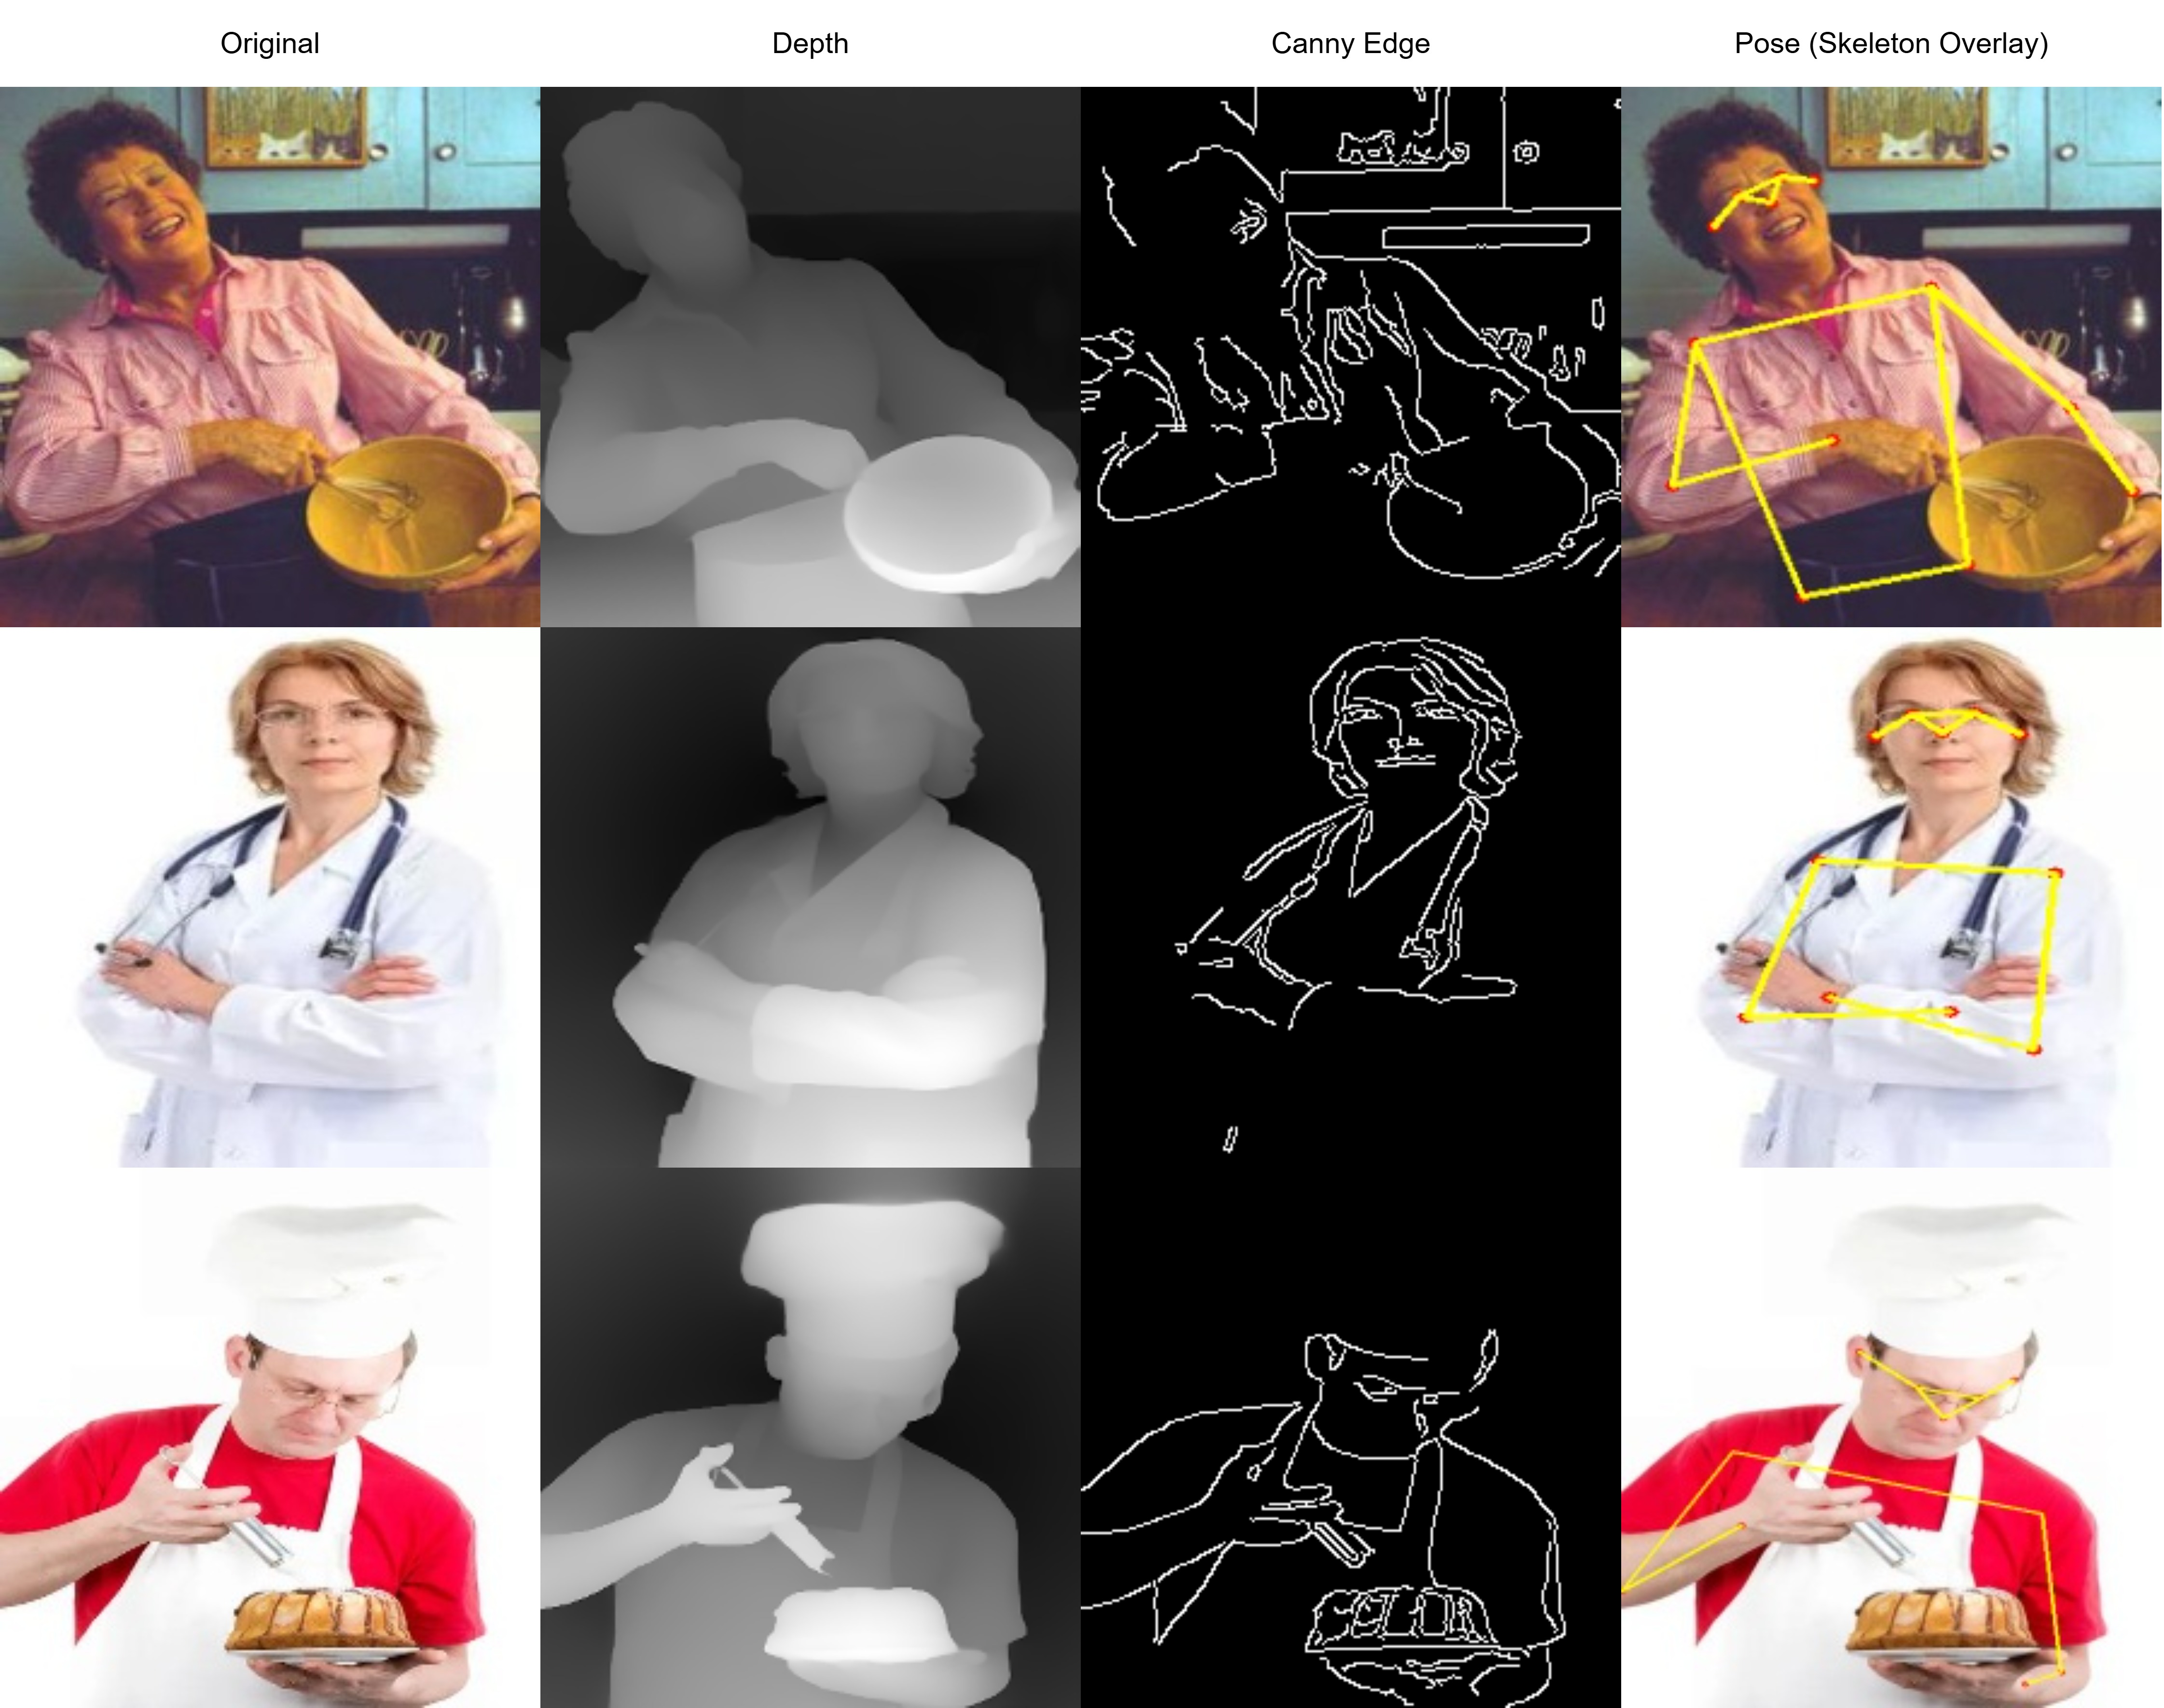
\includegraphics[width=\textwidth]{TD1.jpg}
	\caption{Representative outputs of three structural transformation 
		pipelines applied to the same set of profession-conditioned images. 
		\emph{Depth}: dense relative depth map produced by 
		Depth-Anything-V2 Small, encoding per-pixel scene geometry while 
		suppressing all colour and texture information. 
		\emph{Canny Edge}: sparse boundary map produced by classical Canny 
		edge detection, retaining object contours and spatial intensity 
		discontinuities. 
		\emph{Pose (Skeleton Overlay)}: COCO-17 keypoint skeleton estimated 
		by YOLOv8l-Pose, overlaid on the original image for visual 
		reference; the actual classifier input is the 34-dimensional 
		normalised keypoint vector, not the rendered overlay.}
	\label{fig:td_structural_transforms}
\end{figure}

\subsubsection{Occlusion}
\label{subsec:occlusion}

Occlusion transformations selectively remove or isolate spatial 
regions of each image by replacing either the person or the 
background with a uniform fill, producing a controlled series 
of representations that expose different sources of demographic 
signal. Following the occlusion framework of Meister et 
al.\ \cite{Meister_2023_GenderArtifactsinVisualDatasets}, five 
occlusion variants are produced per image, each isolating a 
distinct combination of person appearance, person geometry, and 
background context. All five variants are applied exclusively to 
Re-LAION-5B and Stable Diffusion v1.5 images as demographic 
probes, testing whether gender and skin tone can be predicted 
from background context alone, from person silhouette geometry 
alone, or from bounding box extent alone, independently of 
pixel-level appearance. COCO images are excluded from the 
occlusion experiments because they are not conditioned on 
occupational queries and are therefore not guaranteed to depict 
people in the professional contexts required for gender and skin 
tone probing. The occlusion pipeline thus operates as a 
two-dataset feature extraction step throughout, consistent with 
the pose estimation pipeline described in 
Section~\ref{subsec:pose}. This work replicates the occlusion 
experiments of Meister et 
al.\ \cite{Meister_2023_GenderArtifactsinVisualDatasets} in 
the context of profession-conditioned imagery and extends them 
to skin tone prediction in addition to gender.

The five variants produced are defined as follows. 
\textbf{Full NoBg} retains the original person pixels within 
the segmentation mask and replaces all background pixels with 
black, isolating person appearance against a neutral background. 
\textbf{MaskSegm} replaces all pixels within the person 
segmentation mask with white while retaining the original 
background, occluding person appearance and exposing background 
context as the sole available signal. \textbf{MaskSegm NoBg} 
replaces person mask pixels with white against a black 
background, retaining only the silhouette shape and spatial 
location of the person with no background or appearance 
information. \textbf{MaskRect} replaces the axis-aligned 
bounding box of the person with white while retaining the 
original background, providing a coarser occlusion of person 
content than the segmentation-based variant. \textbf{MaskRect 
	NoBg} renders a white rectangle corresponding to the person 
bounding box against a black background, retaining only the 
size and location of the person without silhouette detail or 
background context. A sixth variant, Full, which copies the 
unmodified image, was excluded from production runs as it 
produces no transformation. The naming convention follows 
Meister et al.\ \cite{Meister_2023_GenderArtifactsinVisualDatasets} 
directly, where the label refers to what information from the 
person region is preserved --- full person pixels (Full), 
segmentation mask shape (MaskSegm), or bounding box extent 
(MaskRect) --- with NoBg denoting that the background has been 
replaced by a black fill.

A key methodological difference from Meister et al.\ is that 
their analysis operates on COCO images for which ground-truth 
person segmentation masks are available as dataset annotations. 
In this work, the image sets are profession-conditioned 
retrievals from Re-LAION-5B and Stable Diffusion v1.5 outputs, 
for which no ground-truth masks exist. Person masks must 
therefore be predicted by a segmentation model, introducing an 
additional model selection step and a source of mask quality 
variance absent from the original work.

\paragraph{Model Selection}
Five instance segmentation models were evaluated on 
single-person images from the COCO 2017 validation set 
\cite{Lin_2014_COCO} to select the segmentation backbone for 
mask prediction. COCO is used here solely as an evaluation 
benchmark for model selection, providing ground-truth instance 
masks against which predicted masks can be assessed; it does 
not form part of the occlusion transformation experiments 
themselves. The candidates evaluated were Mask2Former with 
COCO instance segmentation weights \cite{Cheng_2022_Mask2Former}, 
Mask2Former with ADE20K semantic segmentation weights, Mask 
R-CNN \cite{He_2017_MaskRCNN}, YOLACT, and Lang-SAM. 
Evaluation measured detection rate (the proportion of images 
for which a non-empty person mask was returned), success rate 
(the proportion of images passing mask and bounding box area 
quality thresholds), mean Intersection over Union against COCO 
ground-truth masks, mask precision and recall, and inference 
throughput. Table~\ref{tab:occlusion_model_eval} summarises 
all results.

\begin{table}[htbp]
	\centering
	\caption{Segmentation model evaluation on single-person 
		images from the COCO 2017 validation set, used 
		for model selection only. Detection rate is the 
		proportion of images for which a non-empty mask was 
		returned. Success rate is the proportion passing mask 
		and bounding box area quality thresholds. IoU, 
		precision, and recall are computed against COCO 
		ground-truth instance masks. Throughput is measured 
		end-to-end on a single GPU.}
	\label{tab:occlusion_model_eval}
	\begin{tabular}{lccccc}
		\hline
		\textbf{Model} & \textbf{Det.\ Rate} & 
		\textbf{Success Rate} & \textbf{IoU} & 
		\textbf{Prec.} & \textbf{Throughput} \\
		\hline
		\textbf{Mask2Former COCO} & \textbf{0.965} & 0.698 & 0.829 & 0.899 & 1.28 it/s \\
		Mask R-CNN                & 0.941 & \textbf{0.707} & 0.813 & ---   & 1.63 it/s \\
		Lang-SAM                  & 0.891 & 0.637 & \textbf{0.846} & \textbf{0.931} & 0.35 it/s \\
		Mask2Former ADE20K        & 0.946 & 0.676 & 0.785 & ---   & 1.86 it/s \\
		YOLACT                    & 0.795 & 0.613 & 0.789 & ---   & 3.00 it/s \\
		\hline
	\end{tabular}
\end{table}

YOLACT was excluded on detection rate grounds: at 79.5\% it 
missed approximately one in five persons in the evaluation set, 
making it unsuitable for a corpus in which missed detections 
propagate directly to missing occlusion outputs across all five 
variants simultaneously. Lang-SAM achieved the highest IoU 
(0.846) and precision (0.931), but at 0.35 iterations per 
second its throughput is approximately 3.7 times slower than 
Mask2Former COCO and nearly five times slower than Mask R-CNN, 
rendering it impractical at full dataset scale. Mask2Former 
ADE20K was excluded despite competitive throughput: it performs 
semantic rather than instance segmentation, treating all person 
pixels as a single undifferentiated class. In images containing 
multiple people, this conflates all person regions into a single 
mask, violating the single-person constraint applied throughout 
the probing pipeline.

Mask R-CNN achieved the highest success rate at 70.7\% and the 
second-highest throughput at 1.63 iterations per second, but 
its detection rate of 94.1\% trails Mask2Former COCO by 2.4 
percentage points --- a gap that compounds significantly at 
corpus scale, as each missed detection produces no occlusion 
output for that image across all five variants. 
\textbf{Mask2Former COCO} was therefore selected on the basis 
of its detection rate of 96.5\% --- the highest of any 
evaluated model --- combined with an IoU of 0.829, precision 
of 0.899, and recall of 0.906, confirming that its masks are 
both reliable and geometrically accurate. Its throughput of 
1.28 iterations per second is lower than Mask R-CNN but 
acceptable given that occlusion generation is a one-time 
offline preprocessing step. Inference was performed at a fixed 
$224 \times 224$ pixel input resolution, which preliminary 
evaluation confirmed to produce no measurable degradation in 
mask quality for this model relative to its native resolution, 
while substantially reducing memory usage.

\paragraph{Occlusion Generation Pipeline}
For each image, Mask2Former COCO was applied in half-precision 
(FP16) under \texttt{torch.no\_grad()} to produce a binary 
person mask at the fixed inference resolution. The predicted 
mask was upsampled to the original image dimensions using 
nearest-neighbour interpolation (\texttt{cv2.INTER\_NEAREST}), 
preserving discrete mask boundaries without introducing 
interpolation artefacts at mask edges. The five occlusion 
variants were then derived from the upsampled mask as 
element-wise operations on the original RGB image. For the 
segmentation-based variants, the mask boundary follows the 
predicted instance silhouette; for the rectangular variants, 
the axis-aligned bounding box is computed as the minimum 
enclosing rectangle of all foreground mask pixels, with corners 
at $(\min x_s, \min y_s)$ and $(\max x_s, \max y_s)$ over the 
set of foreground pixel coordinates $\{(x_s, y_s)\}$. All 
occlusion fills use a uniform white value (RGB $= [255, 255, 
255]$) for masked regions and black (RGB $= [0, 0, 0]$) for 
background suppression, consistent with the convention of 
Meister et al.\ 
\cite{Meister_2023_GenderArtifactsinVisualDatasets}, who 
demonstrate that results are robust to the choice of fill 
colour. Final output images were resized to $224 \times 224$ 
pixels via bilinear interpolation for compatibility with the 
downstream classifier. Mask area ratios and bounding box area 
ratios were recorded to a quality control CSV file per image. 
The pipeline is fully resumable via an append-only JSONL 
manifest that tracks completed operations per image, enabling 
fault-tolerant processing across the full two-dataset corpus.

Representative segmentation-based occlusion outputs are shown 
in Figure~\ref{fig:td_segmentation_occlusion}, and rectangular 
occlusion outputs in Figure~\ref{fig:td_occlusion_rect}.

\begin{figure}[htbp]
	\centering
	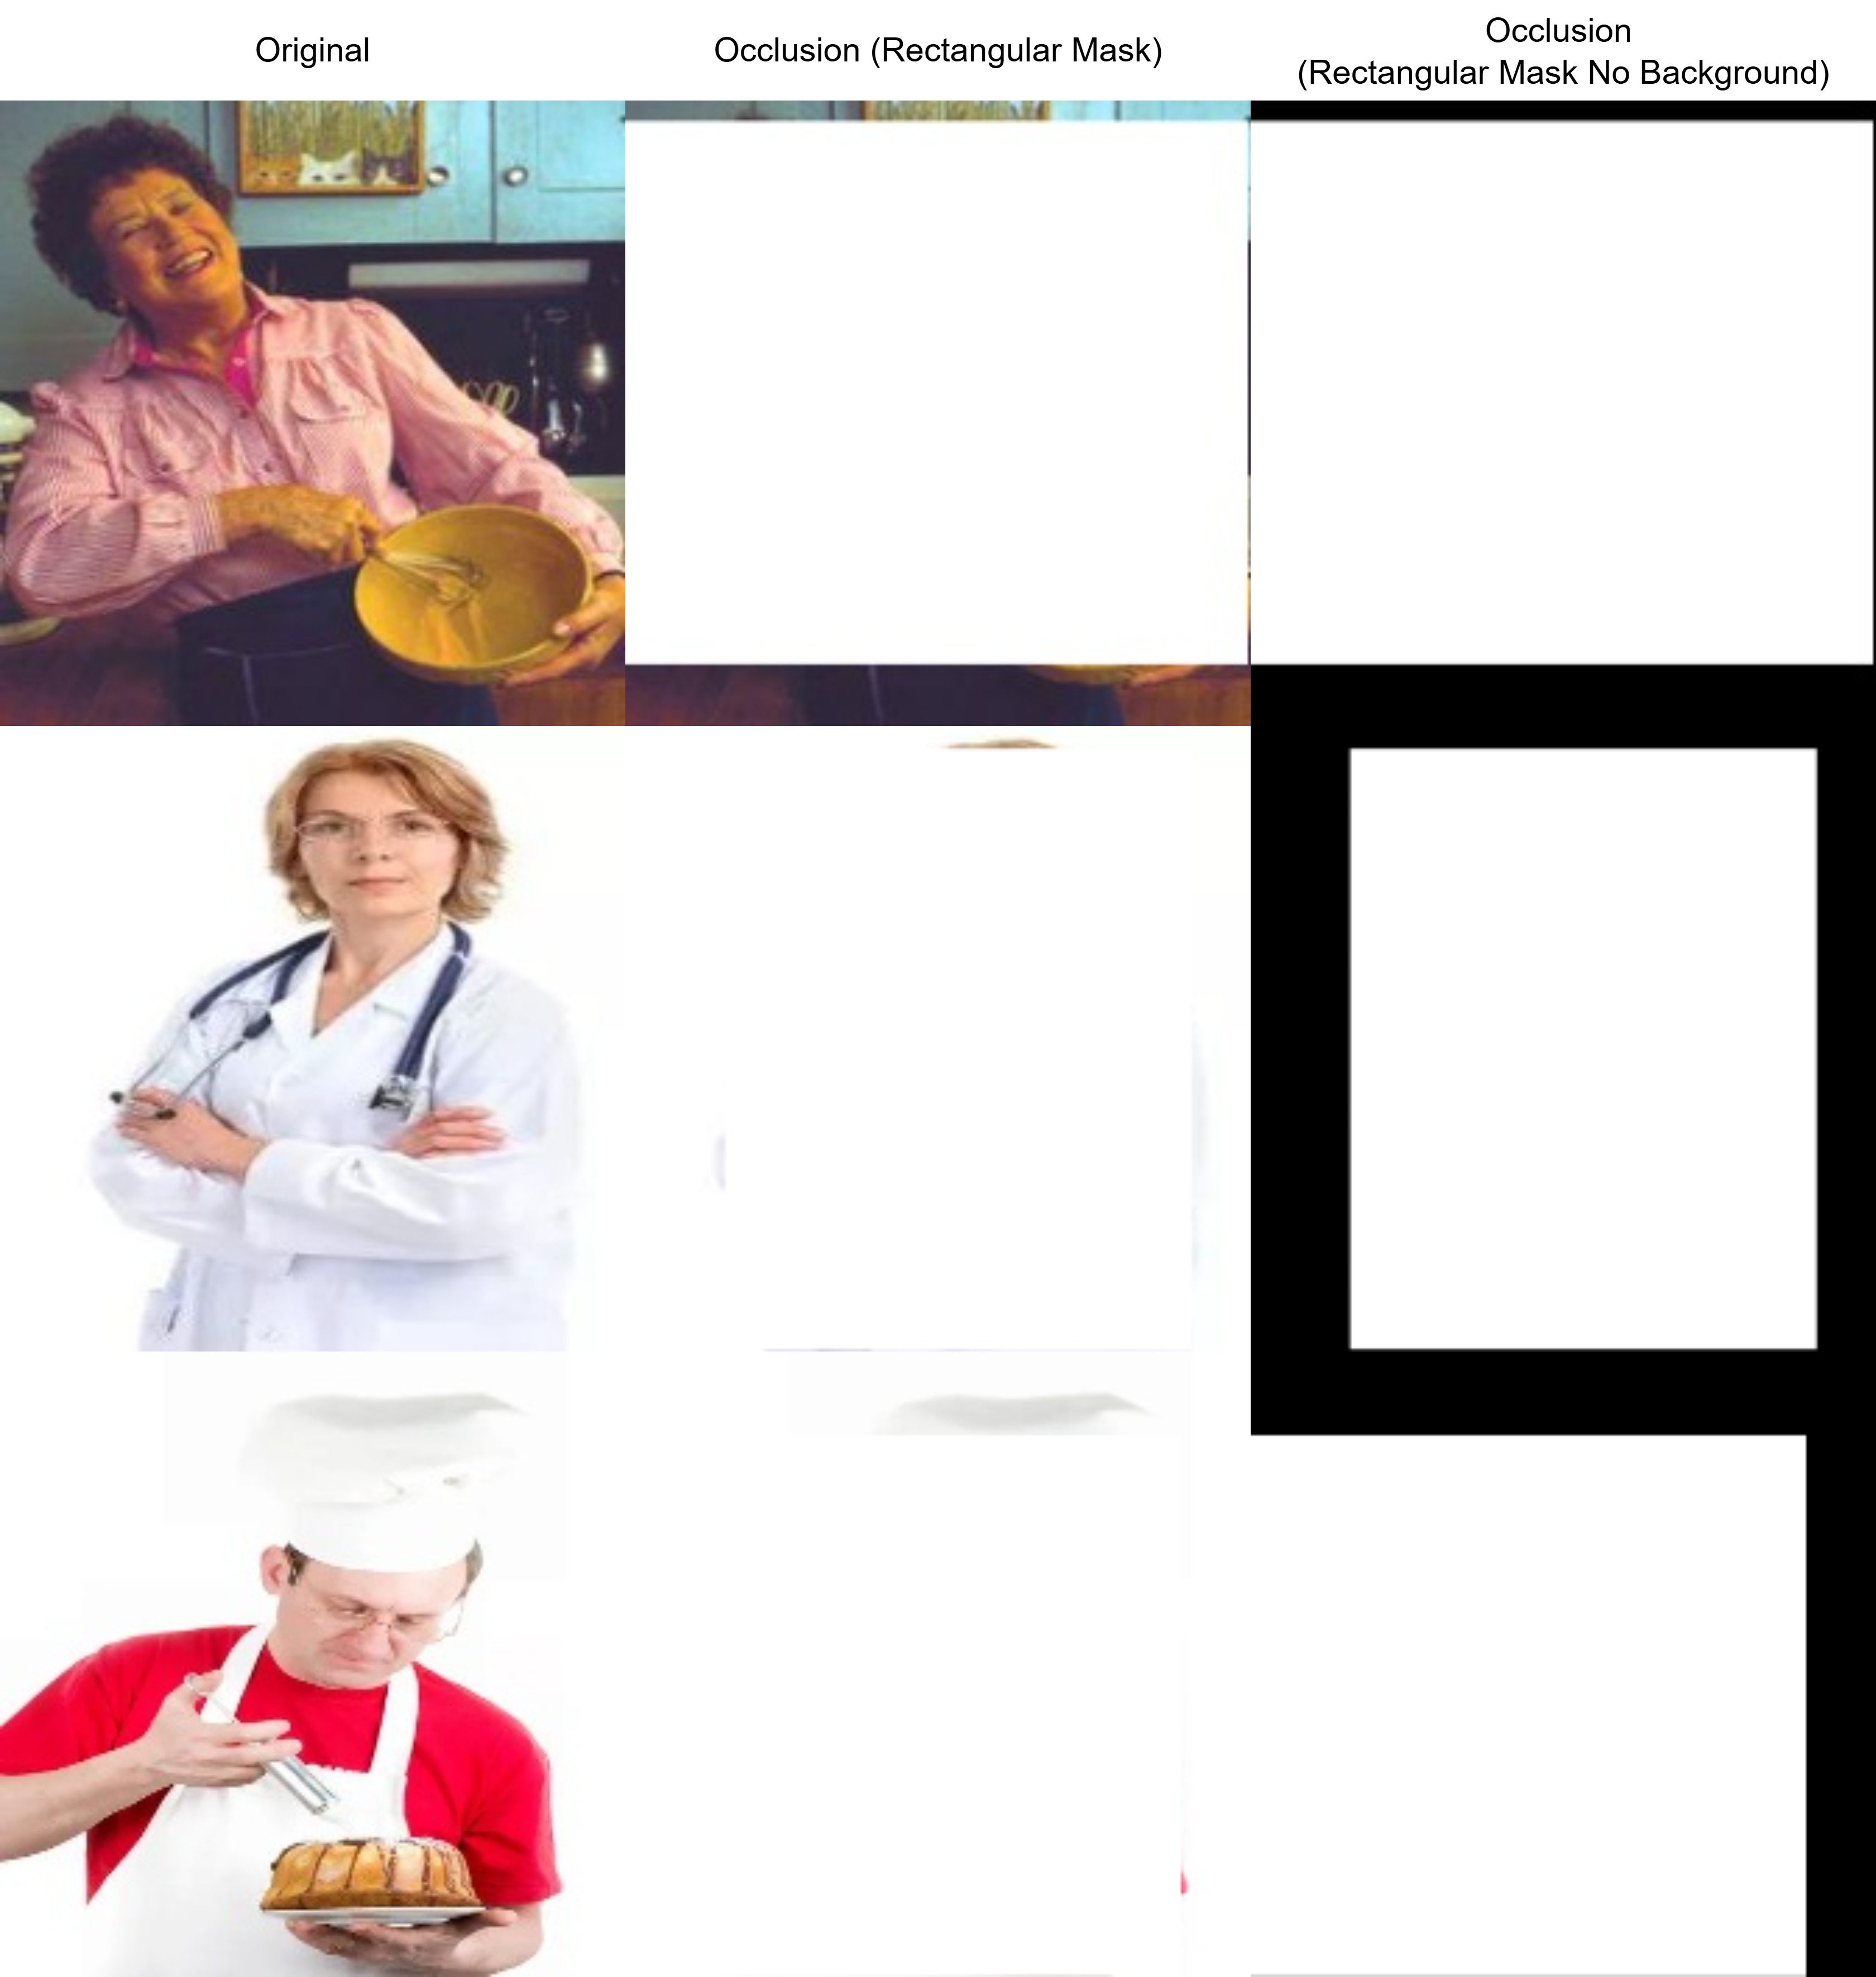
\includegraphics[width=0.75\textwidth]{TD6.jpg}
	\caption{Rectangular occlusion transformations applied to three 
		profession-conditioned images. 
		\emph{Occlusion (Rectangular Mask)}: the subject region replaced 
		by a uniform white rectangle, removing the person while preserving 
		background context. 
		\emph{Occlusion (Rectangular Mask No Background)}: the inverse 
		mask applied with a black background, retaining only the occluded 
		region boundary.}
	\label{fig:td_occlusion_rect}
\end{figure}



\section{Inference-Time Debiasing of Stable Diffusion v1.5}
\label{sec:debiased_generation}

The preceding analyses characterise the spurious features and 
demographic biases present in Re-LAION-5B and in the standard 
Stable Diffusion v1.5 generation pipeline. A complementary 
question is whether inference-time debiasing interventions 
applied to the same base model can produce measurable shifts 
in its demographic output distribution. This section describes 
the debiased generation pipeline used to produce a 
10{,}000-image corpus against which the effectiveness of these 
interventions is evaluated in Section~\ref{sec:evaluation}.

A range of approaches to mitigating demographic bias in 
text-to-image diffusion models has been proposed in the 
literature, broadly falling into three categories: retraining 
or fine-tuning on demographically balanced corpora, which 
achieves thorough debiasing at the cost of substantial compute 
and curated reference data; weight editing methods such as 
Unified Concept Editing \cite{Gandikota_2024_UCE}, which 
directly modify cross-attention projections to remove targeted 
concept associations; and inference-time interventions, which 
steer generation without altering model weights and are 
therefore applicable to any frozen pretrained model. Given the 
computational constraints of this work and the requirement that 
the base model remain Stable Diffusion v1.5 to preserve the 
documentable link to Re-LAION-5B, the analysis is restricted 
to inference-time approaches. Retraining and weight editing 
methods are acknowledged as potentially more thorough 
interventions but are outside the scope of the present 
evaluation.

\subsection{Experimental Design}
\label{subsec:debias_design}

The debiased corpus consists of 10{,}000 images generated for 
a single profession --- \textit{doctor} --- rather than 
distributed across the full 200-profession list used in the 
standard generation pipeline. This design choice is motivated 
by the analytical objective of the experiment: the goal is to 
isolate the effect of the debiasing interventions themselves, 
not to reproduce the full profession-conditioned corpus under 
a different generation regime. Spreading 10{,}000 images 
across 200 professions yields only 50 images per profession 
per demographic condition, and any observed demographic shift 
would be confounded by the profession-specific demographic 
priors already embedded in the model --- the baseline gender 
distribution for \textit{nurse} differs substantially from 
that of \textit{engineer} regardless of debiasing, making it 
impossible to cleanly attribute observed distributional shifts 
to the intervention. Concentrating all 10{,}000 images on a 
single profession eliminates this confound, provides 
substantially higher statistical power per demographic 
condition, and produces a comparison between the standard and 
debiased corpora that is directly attributable to the 
generation pipeline rather than to profession sampling. The 
\textit{doctor} profession was selected because it exhibits 
a well-documented male skew in text-to-image model outputs, 
making it a meaningful and sensitive test case for 
debiasing effectiveness.

The same structural validation pipeline applied to the 
standard generated image set is applied here, ensuring 
that the debiased corpus is filtered to identical quality 
criteria and that demographic annotation is performed under 
identical conditions, enabling direct distributional 
comparison.

\subsection{ITI-GEN Demographic Conditioning}
\label{subsec:itigen}

ITI-GEN \cite{Zhang_2023_ITIGEN} augments the text 
conditioning signal by prepending learned inclusive token 
embeddings to the prompt representation at inference time. 
These embeddings are trained on a reference image corpus to 
span the demographic attribute combinations of interest, 
steering the diffusion model toward more balanced demographic 
outputs without modifying its weights. This approach is 
directly compatible with any frozen Stable Diffusion 
checkpoint and imposes no additional inference overhead 
beyond the embedding lookup and concatenation.

Token embeddings were trained on the CCv2 dataset 
\cite{TODO_CCv2} using two attribute axes: 
\texttt{CCv2\_Gender} (female, male) and 
\texttt{CCv2\_MSTE\_SkinTone} (spanning the ten-point Monk 
Skin Tone scale), producing a set of learned perturbation 
embeddings indexed over all gender--skin tone combinations. 
The training prompt was \texttt{"an image of a person"}, 
following the ITI-GEN convention of using a neutral 
descriptive prompt for embedding training. Embeddings were 
loaded from a checkpoint at epoch 19 and applied to the 
generation prompt \texttt{"A picture of a doctor"} via the 
\texttt{prompt\_prepend} mechanism, which concatenates the 
inclusive embeddings with the CLIP text encoding of the 
generation prompt before passing the combined representation 
to the UNet cross-attention layers.

\subsection{Pose Conditioning via ControlNet}
\label{subsec:debias_controlnet}

A fixed canonical pose was enforced across all debiased 
generated images using ControlNet \cite{LZhang_2023_ControlNet} 
with an OpenPose conditioning signal 
(\texttt{lllyasviel/control\_v11p\_sd15\_openpose}). The 
conditioning image was a single reference pose skeleton 
(\texttt{basic\_pose.jpg}) depicting a neutral standing 
figure, applied at a ControlNet scale of 0.8 for all 
10{,}000 images.

Pose conditioning serves a specific methodological purpose 
in the debiasing evaluation. Without a fixed structural 
constraint, the model's learned pose prior may itself be 
demographically skewed: if the model associates certain 
genders or skin tones with particular poses, variations 
in body geometry across generated images could introduce 
a confound into the demographic annotation pipeline. 
Enforcing a canonical pose across all images ensures that 
any observed demographic variation in the debiased corpus 
reflects differences in appearance-level attributes --- 
gender expression and skin tone --- rather than 
pose-correlated compositional differences. This is 
consistent with the structural normalisation applied in 
the pose estimation probing pipeline 
(Section~\ref{subsec:pose}), where keypoints are 
normalised to remove scale and position cues precisely 
to prevent pose geometry from acting as a demographic 
proxy.

\subsection{Colour Alignment}
\label{subsec:colour_alignment}

ITI-GEN operates at the level of semantic text conditioning 
and does not directly constrain the colour distribution of 
generated images. A complementary inference-time colour 
alignment strategy was therefore added to steer the 
denoising trajectory in latent space toward the colour 
distribution of a skin-tone-diverse reference image, 
providing a low-level signal that reinforces the semantic 
demographic conditioning. Two colour alignment approaches 
were implemented and compared prior to selecting one for 
full-scale generation.

\paragraph{SW-Guidance}
The first approach applies Sliced Wasserstein Distance 
(SWD) guidance at each denoising step. At a configurable 
decode-start timestep, the current latent is decoded to 
pixel space, and a gradient signal is computed by 
minimising the SWD between the decoded image's colour 
distribution and that of a reference image. This gradient 
is used to update an auxiliary latent variable via gradient 
ascent, with the corrected latent reinjected into the 
denoising trajectory. Multiple SWD variants were evaluated, 
including standard SWD, Distributional SWD (DSWD), 
Generalised SWD (GSWD), and ISEBSW, alongside optional 
time-travel blocks that re-introduce forward noise steps 
to allow iterative correction. Despite producing visually 
favourable colour distributions in preliminary qualitative 
evaluation --- with outputs arguably exhibiting more 
natural skin tone variation than the Chamfer approach --- 
SW-Guidance was excluded from full-scale generation on 
throughput grounds. The repeated decode--gradient--encode 
operations at each denoising step result in inference 
times incompatible with generating 10{,}000 images within 
the available computational window.

\paragraph{Chamfer Colour Alignment}
The second approach performs colour steering directly in 
latent space without decoding to pixels at each step. A 
reference image is blurred with a Gaussian filter and 
encoded to a latent representation at the start of 
generation. At each DDPM backward step, the predicted 
clean sample $\hat{x}_0$ is projected toward the reference 
latent distribution using an iterative Chamfer distance 
matching procedure: nearest-neighbour correspondences 
between the spatial positions of the current latent and 
the reference latent are established via $k$-nearest 
neighbour search, a displacement field is computed from 
the matched correspondences, matched reference points are 
peeled from the candidate set to prevent degenerate 
collapse, and the projected latent is blended back into 
the denoising step via a learning-rate-scaled update. 
This projection is applied inside the DDPM backward step 
at each timestep, following the zero-shot colour alignment 
placement of Couairon et 
al.\ \cite{Couairon_2022_ZeroShotImageToImage}. Because 
the Chamfer projection operates entirely within the 
$4 \times H/8 \times W/8$ latent space, it imposes no 
additional decode--encode overhead per step and achieves 
throughput comparable to standard generation. Chamfer 
colour alignment was accordingly selected for the 
full-scale debiased generation run.

\subsection{Generation Configuration}
\label{subsec:debias_config}

\textbf{NOTE:} Section to be written once images are generated

%The final debiased generation pipeline combines four 
%components operating on the Stable Diffusion v1.5 base 
%model: ITI-GEN demographic conditioning, OpenPose 
%ControlNet structural conditioning, Chamfer latent-space 
%colour alignment, and LCM-LoRA acceleration. Preliminary 
%evaluation confirmed that the Chamfer latent-space 
%projection is fully compatible with the four-step LCM 
%schedule, producing structurally valid images across all 
%demographic attribute combinations, ControlNet conditioning 
%configurations, and colour alignment settings. Generation 
%therefore used the same four-step LCM inference schedule 
%and guidance scale of 1.0 as the standard generation 
%pipeline, with 8 inference steps, ensuring that any 
%observed differences in demographic output distributions 
%are attributable to the debiasing interventions rather 
%than to generation configuration differences.
%
%Colour alignment used a blurred pastel reference image 
%as the alignment target, selected to provide a neutral, 
%skin-tone-diverse colour palette without introducing 
%domain-specific semantic content into the colour guidance 
%signal. Projection hyperparameters were set to a threshold 
%of 200, a learning rate of 0.3, and a Gaussian blur factor 
%of 3, determined through preliminary qualitative 
%evaluation. The ControlNet conditioning scale was set to 
%0.8, providing strong structural guidance while permitting 
%sufficient generative freedom for appearance-level 
%demographic variation. The generation prompt 
%\texttt{"A picture of a doctor"} was used throughout, 
%consistent with the exploratory runs used to validate 
%the pipeline. Results of the demographic annotation 
%applied to this corpus and its comparison with the 
%standard Stable Diffusion v1.5 generation corpus are 
%reported in Section~\ref{sec:evaluation}.